% !TeX root = surgery.tex
%\RequirePackage{snapshot}
% !TeX encoding = UTF-8
% !TeX spellcheck = en_GB
\documentclass[12pt,draft]{article} %taking out draft switches off marginal notes

\usepackage{../incremental_SS_Translation} % all customizations in this file


\addbibresource{../incremental_SS_Translation.bib}

\usepackage{xcolor}

\title{The \SS\ on the Plastic Surgery of the Ears and Nose:\\ The Nepalese 
Recension}
\author{Dominik Wujastyk, 
Jason Birch,
Andrey Klebanov, \\
Madhu Parameswaran,
Madhusudan Rimal, 
Deepro Chakraborty,\\
Harshal Bhatt, 
Devyani Shenoy,
Vandana Lele.}
\date{\texttt{Draft of \today}\\ \copyright\     \small{Dominik Wujastyk, 
Jason Birch,
Andrey Klebanov, 
Madhu Parameswaran,
Madhusudan Rimal, 
Deepro Chakraborty,
Harshal Bhatt, 
Devyani Shenoy,
Vandana Lele.}}

\begin{document}
 
    % Manual hyphenation points for Sanskrit words and compounds.
% By Dominik Wujastyk.
% Copyright Dominik Wujastyk 2021.
% Released under a BY-SA Creative Commons license 
% (Attribution-ShareAlike 4.0 International http://creativecommons.org/licenses/by-sa/4.0/).
% This file is still actively growing, slowly but steadily (March 2021) .
%
% These special hyphenations have to be loaded after
% \begin{document}. See
% http://www.tug.org/pipermail/xetex/2008-July/010362.html
% Or use 
% \AtBeginDocument{% Manual hyphenation points for Sanskrit words and compounds.
% By Dominik Wujastyk.
% Copyright Dominik Wujastyk 2021.
% Released under a BY-SA Creative Commons license 
% (Attribution-ShareAlike 4.0 International http://creativecommons.org/licenses/by-sa/4.0/).
% This file is still actively growing, slowly but steadily (March 2021) .
%
% These special hyphenations have to be loaded after
% \begin{document}. See
% http://www.tug.org/pipermail/xetex/2008-July/010362.html
% Or use 
% \AtBeginDocument{% Manual hyphenation points for Sanskrit words and compounds.
% By Dominik Wujastyk.
% Copyright Dominik Wujastyk 2021.
% Released under a BY-SA Creative Commons license 
% (Attribution-ShareAlike 4.0 International http://creativecommons.org/licenses/by-sa/4.0/).
% This file is still actively growing, slowly but steadily (March 2021) .
%
% These special hyphenations have to be loaded after
% \begin{document}. See
% http://www.tug.org/pipermail/xetex/2008-July/010362.html
% Or use 
% \AtBeginDocument{\input{sanskrit-hyphenations}}% should work, but doesn't
% special hyphenations for Sanskrit words tagged in
% Polyglossia.
% *English,\textenglish{},text,and
% *Sanskrit,\textsanskrit{},text.
%
% English (see below for \textsanskrit)
%
\hyphenation{%
    dhanva-ntariṇopa-diṣ-ṭaḥ
    suśruta-nāma-dheyena
    tac-chiṣyeṇa
    kāśyapa-saṃ-hitā
    cikitsā-sthāna
    su-śruta-san-dīpana-bhāṣya
    dṛṣṭi-maṇḍala
    uc-chiṅga-na
    sarva-siddhānta-tattva-cūḍā-maṇi
    tulya-sau-vīrāñja-na
    indra-gopa
    śrī-mad-abhi-nava-guptā-cārya-vi-ra-cita-vi-vṛti-same-tam
    viśva-nātha
śrī-mad-devī-bhāga-vata-mahā-purāṇa
    siddhā-n-ta-sun-dara
    brāhma-sphuṭa-siddh-ānta
    bhū-ta-saṅ-khyā
    bhū-ta-saṃ-khyā
    kathi-ta-pada
    devī-bhā-ga-vata-purāṇa
    devī-bhā-ga-vata-mahā-purāṇa
    Siddhānta-saṃ-hitā-sāra-sam-uc-caya
    sau-ra-pau-rāṇi-ka-mata-sam-artha-na
    Pṛthū-da-ka-svā-min
    Brah-ma-gupta
    Brāh-ma-sphu-ṭa-siddhānta
    siddhānta-sun-dara
    vāsa-nā-bhāṣya
    catur-veda
    bhū-maṇḍala
    jñāna-rāja
    graha-gaṇi-ta-cintā-maṇi
    Śiṣya-dhī-vṛd-dhi-da-tan-tra
    brah-māṇḍa-pu-rā-ṇa
    kūr-ma-pu-rā-ṇa
    jam-bū-dvī-pa
    bhā-ga-vata-pu-rā-ṇa
    kupya-ka
    nandi-suttam
    nandi-sutta
    su-bodhiā-bāī
    asaṅ-khyāta
    saṅ-khyāta
    saṅ-khyā-pra-māṇa
    saṃ-khā-pamāṇa
    nemi-chandra
    anu-yoga-dvāra
    tattvārtha-vārtika
    aka-laṅka
    tri-loka-sāra
    gaṇi-ma-pra-māṇa
    gaṇi-ma-ppa-māṇa
    eka-pra-bhṛti
gaṇaṇā-saṃ-khā
gaṇaṇā-saṅ-khyā
dvi-pra-bhṛti
duppa-bhi-ti-saṃ-khā
vedanābhi-ghāta
Viṣṇu-dharmottara-pu-rāṇa
abhaya-deva-sūri-vi-racita-vṛtti-vi-bhūṣi-tam
abhi-dhar-ma
abhi-dhar-ma-ko-śa
abhi-dhar-ma-ko-śa-bhā-ṣya
abhi-dharma-kośa-bhāṣya
abhi-dharma-kośa-bhāṣyam
abhi-nava
abhyaṃ-karopāhva-vāsu-deva-śāstri-vi-ra-ci-ta-yā
ācārya-śrī-jina-vijayālekhitāgra-vacanālaṃ-kṛtaś-ca
ācāry-opā-hvena
ādhāra
adhi-kāra
adhi-kāras
ādi-nātha
agni-besha
agni-veśa
ahir-budhnya
ahir-budhnya-saṃ-hitā
aita-reya-brāhma-ṇa
akusī-dasya
amara-bharati
Amar-augha-pra-bo-dha
amṛ-ta-siddhi
ānanda-kanda
ānan-da-rā-ya
ānand-āśra-ma-mudraṇā-la-ya
ānand-āśra-ma-saṃ-skṛta-granth-āva-liḥ
anna-pāna-mūlā
anu-ban-dhya-lakṣaṇa-sam-anv-itās
anu-bhav-ād
anu-bhū-ta-viṣayā-sam-pra-moṣa
anu-bhū-ta-viṣayā-sam-pra-moṣaḥ
aparo-kṣā-nu-bhū-ti
app-proxi-mate-ly
ardha-rātrika-karaṇa
ārdha-rātrika-karaṇa
ariya-pary-esana-sutta
arun-dhatī
ārya-bhaṭa
ārya-bhaṭā-cārya-vi-racitam
ārya-bhaṭīya
ārya-bhaṭīyaṃ
ārya-lalita-vistara-nāma-mahā-yāna-sūtra
ārya-mañju-śrī-mūla-kalpa
ārya-mañju-śrī-mūla-kalpaḥ
asaṃ-pra-moṣa
aṣṭāṅga-hṛdaya-saṃ-hitā
aṣṭāṅga-saṃ-graha
asura-bhavana
aśva-ghoṣa
ātaṅka-darpaṇa-vyā-khyā-yā
atha-vā
ava-sāda-na
āyār-aṅga-suttaṃ
ayur-ved
ayur-veda
āyur-veda
āyur-veda-dīpikā
āyur-veda-dīpikā-vyā-khyayā
āyur-ve-da-ra-sā-yana
āyur-veda-sū-tra
ayur-vedic
āyur-vedic
ayur-yog
bādhirya
bahir-deśa-ka
bala-bhadra
bala-kot
bala-krishnan
bāla-kṛṣṇa
bau-dhā-yana-dhar-ma-sūtra
bel-valkar
bhadra-kālī-man-tra-vi-dhi-pra-karaṇa
bhadrā-sana
bhadrā-sanam
bha-ga-vat-pāda
bhaiṣajya-ratnāvalī
bhan-d-ar-kar
bhartṛhari-viracitaḥ
bhaṭṭā-cārya
bhaṭṭot-pala-vi-vṛti-sahitā
Bhiṣag-varāḍha-malla-vi-racita-dīpikā-Kāśī-rāma-vaidya-vi-raci-ta-gūḍhā-rtha-dīpikā-bhyāṃ
bhiṣag-varāḍha-malla-vi-racita-dīpikā-Kāśī-rāma-vaidya-vi-racita-gūḍhārtha-dīpikā-bhyāṃ
bhoja-deva-vi-raci-ta-rāja-mārtaṇḍā-bhi-dha-vṛtti-sam-e-tāni
bhu--va-na-dī-pa-ka
bīja-pallava
bi-kaner
bodhi-sat-tva-bhūmi
brahma-gupta
brahmā-nanda
brahmāṇḍa-mahā-purā-ṇa
brahmāṇḍa-mahā-purā-ṇam
brahma-randhra
brahma-siddh-ānta
brāhma-sphuṭa-siddh-ānta
brāhma-sphu-ṭa-siddhānta
brahma-vi-hāra
brahma-vi-hāras
brahma-yā-mala-tan-tra
Bra-ja-bhāṣā
bṛhad-āraṇya-ka
bṛhad-yā-trā
bṛhad-yogi-yājña-valkya-smṛti
bṛhad-yogī-yājña-valkya-smṛti
bṛhaj-jāta-kam
bṛhat-khe-carī-pra-kāśa
buddhi-tattva-pra-karaṇa
cak-ra-dat-ta
cakra-datta
cakra-pāṇi-datta
cā-luk-ya
caraka-prati-saṃ-s-kṛta
caraka-prati-saṃ-s-kṛte
caraka-saṃ-hitā
casam-ul-lasi-tāmaharṣiṇāsu-śrutenavi-raci-tāsu-śruta-saṃ-hitā
cau-kham-ba
cau-luk-yas
chandi-garh
chara-ka
cha-rīre
chatt-opa-dh-ya-ya
chau-kham-bha
chi-ki-tsi-ta
cid-ghanā-nanda-nātha
ci-ka-ner
com-men-taries
com-men-tary
com-pre-hen-sive-ly
daiva-jñālaṃ-kṛti
daiva-jñālaṅ-kṛti
dāmo-dara-sūnu-Śārṅga-dharācārya-vi-racitā
Dāmodara-sūnu-Śārṅga-dharācārya-vi-racitā
darśanā-ṅkur-ābhi-dhayā
das-gupta
deha-madhya
deha-saṃ-bhava-hetavaḥ
deva-datta
deva-nagari
deva-nāgarī
devā-sura-siddha-gaṇaiḥ
dha-ra-ni-dhar
dharma-megha
dharma-meghaḥ
dhru-vam
dhru-va-sya
dhru-va-yonir
dhyā-na-grahopa-deśā-dhyā-yaś
dṛḍha-śūla-yukta-rakta
dvy-ulbaṇaikolba-ṇ-aiḥ
four-fold
gan-dh-ā-ra
gārgīya-jyoti-ṣa
gārgya-ke-rala-nīla-kaṇṭha-so-ma-sutva-vi-racita-bhāṣyo-pe-tam
garuḍa-mahā-purāṇa
gaurī-kāñcali-kā-tan-tra
gau-tama
gauta-mādi-tra-yo-da-śa-smṛty-ātma-kaḥ
gheraṇḍa-saṃ-hitā
gorakṣa-śata-ka
go-tama
granth-ā-laya
grantha-mālā
gran-tha-śreṇiḥ
grāsa-pramāṇa
guru-maṇḍala-grantha-mālā
gyatso
hari-śāstrī
haṭhābhyāsa-paddhati
haṭha-ratnā-valī
Haṭha-saṅ-keta-candri-kā
haṭha-tattva-kau-mudī
haṭha-yoga
hāyana-rat-na
haya-ta-gran-tha
hema-pra-bha-sūri
hetu-lakṣaṇa-saṃ-sargād
hīna-madhyādhi-kaiś
hindī-vyā-khyā-vi-marśope-taḥ
hoern-le
ijya-rkṣa
ikka-vālaga
indra-dhvaja
indrāṇī-kalpa
indria
Īśāna-śiva-guru-deva-pad-dhati
jābāla-darśanopa-ni-ṣad
jadav-ji
jagan-nā-tha
jala-basti
jal-pa-kal-pa-tāru
jam-bū-dvī-pa-pra-jña-pti
jam-bū-dvī-pa-pra-jña-pti-sūtra
jana-pad-a-sya
jāta-ka-kar-ma-pad-dhati
jaya-siṃha
jinā-agama-grantha-mālā
jin-en-dra-bud-dhi
jīvan-muk-ti-vi-veka
jñā-na-nir-mala
jñā-na-nir-malaṃ
joga-pra-dīpya-kā
jya-rkṣe
Jyo-tiḥ-śās-tra
jyo-ti-ṣa-rāya
jyoti-ṣa-rāya
jyotiṣa-siddhānta-saṃ-graha
jyotiṣa-siddhānta-saṅ-graha
kāka-caṇḍīśvara-kal-pa-tan-tra
kakṣa-puṭa
kali-kāla-sarva-jña
kali-kāla-sarva-jña-śrī-hema-candrācārya-vi-raci-ta
kali-kāla-sarva-jña-śrī-hema-candrācārya-vi-raci-taḥ
kali-yuga
kal-pa
kal-pa-sthāna
kalyāṇa-kāraka
Kāmeśva-ra-siṃha-dara-bhaṅgā-saṃ-skṛta-viśva-vidyā-layaḥ
kapāla-bhāti
karaṇa-tilaka
kar-ma
kar-man
kāṭhaka-saṃ-hitā
kavia-rasu
kavi-raj
keśa-va-śāstrī
ke-vala--rāma
keva-la-rāma
khaṇḍa-khādyaka-tappā
khe-carī-vidyā
knowl-edge
kol-ka-ta
kriyā-krama-karī
kṛṣṇa-pakṣa
kṛtti-kā
kṛtti-kās
kubji-kā-mata-tantra
kula-pañji-kā
kul-karni
ku-māra-saṃ-bhava
kuṭi-pra-veśa
kuṭi-pra-veśika
lakṣ-mī-veṅ-kaṭ-e-ś-va-ra
lit-era-ture
lit-era-tures
locana-roga
mādha-va
mādhava-kara
mādhava-ni-dāna
mādhava-ni-dā-nam
madh-ūni
madhya
mādhyan-dina
madhye
mahā-bhāra-ta
mahā-deva
mahā-kavi-bhartṛ-hari-praṇīta-tvena
maha-mahopa-dhyaya
mahā-maho-pā-dhyā-ya-śrī-vi-jñā-na-bhikṣu-vi-raci-taṃ
mahā-mati-śrī-mādhava-kara-pra-ṇī-taṃ
mahā-mudrā
mahā-muni-śrī-mad-vyāsa-pra-ṇī-ta
mahā-muni-śrī-mad-vyāsa-pra-ṇī-taṃ
maharṣiṇā
maha-rṣi-pra-ṇīta-dharma-śāstra-saṃ-grahaḥ
Maha-rṣi-varya-śrī-yogi-yā-jña-valkya-śiṣya-vi-racitā
mahā-sacca-ka-sutta
mahā-sati-paṭṭhā-na-sutta
mahā-vra-ta
mahā-yāna-sūtrālaṅ-kāra
maitrāya-ṇī-saṃ-hitā
maktab-khānas
māla-jit
māli-nī-vijayot-tara-tan-tra
manaḥ-sam-ā-dhi
mānasol-lāsa
mānava-dharma-śāstra
mandāgni-doṣa
mannar-guḍi
mano-har-lal
mano-ratha-nandin
man-u-script
man-u-scripts
mataṅga-pārame-śvara
mater-ials
matsya-purāṇam
medh-ā-ti-thi
medhā-tithi
mithilā-stha
mithilā-stham
mithilā-sthaṃ
mṛgendra-tantra-vṛtti
mud-rā-yantr-ā-laye
muktā-pīḍa
mūla-pāṭha
muṇḍī-kalpa
mun-sh-ram
Nāda-bindū-pa-ni-ṣat
nāga-bodhi
nāga-buddhi
nakṣa-tra
nara-siṃha
nārā-yaṇa-dāsa
nārā-yaṇa-dāsa
nārā-yaṇa-kaṇṭha
nārā-yaṇa-paṇḍi-ta-kṛtā
nar-ra-tive
nata-rajan
nava-pañca-mayor
nava-re
naya-na-sukho-pā--dhyāya
ni-ban-dha-saṃ-grahā-khya-vyākhya-yā
niban-dha-san-graha
ni-dā-na
nidā-na-sthā-na-sya
ni-dāna-sthānasyaśrī-gaya-dāsācārya-vi-racitayānyāya-candri-kā-khya-pañjikā-vyā-khyayā
nir-anta-ra-pa-da-vyā-khyā
nir-guṇḍī-kalpa
nir-ṇaya-sā-gara
Nir-ṇaya-sāgara
nir-ṇa-ya-sā-gara-mudrā-yantrā-laye
nir-ṇa-ya-sā-ga-ra-yantr-āla-ya
nir-ṇaya-sā-gara-yantr-ā-laye
niśvāsa-kārikā
nīti-śṛṅgāra-vai-rāgyādi-nāmnāsamākhyā-tānāṃ
nityā-nanda
nya-grodha
nya-grodho
nyā-ya-candri-kā-khya-pañji-kā-vyā-khya-yā
nyāya-śās-tra
okaḥ-sātmya
okaḥ-sātmyam
okaḥ-sātmyaṃ
oka-sātmya
oka-sātmyam
oka-sātmyaṃ
oris-sa
oṣṭha-saṃ-puṭa
ousha-da-sala
padma-pra-bha-sūri
Padma-prā-bhṛ-ta-ka
padma-sva-sti-kārdha-candrādike
paitā-maha-siddhā-nta
pañca-karma
pañca-karman
pāñca-rātrā-gama
pañca-siddh-āntikā
paṅkti-śūla
Paraśu-rāma
paraśu-rāma
pari-likh-ya
pāśu-pata-sū-tra-bhāṣya
pātañ-jala-yoga-śās-tra
pātañ-jala-yoga-śās-tra-vi-varaṇa
pat-añ-jali
pat-na
pāva-suya
phiraṅgi-can-dra-cchedyo-pa-yogi-ka
pim-pal-gaon
pipal-gaon
pitta-śleṣ-man
pit-ta-śleṣ-ma-śoṇi-ta
pitta-śoṇi-ta
prā-cīna-rasa-granthaḥ
prā-cya
prā-cya-hindu-gran-tha-śreṇiḥ
prācya-vidyā-saṃ-śodhana-mandira
pra-dhān-in
pra-ka-shan
pra-kaṭa-mūṣā
pra-kṛ-ti-bhū-tāḥ
pra-mā-ṇa-vārt-tika
pra-ṇītā
pra-saṅ-khyāne
pra-śas-ta-pāda-bhāṣya
pra-śna-pra-dīpa
pra-śnārṇa-va-plava
praśnārṇava-plava
pra-śna-vai-ṣṇava
pra-śna-vaiṣṇava
prati-padyate
pra-yatna-śaithilyānan-ta-sam-āpatti-bhyām
prei-sen-danz
punar-vashu
puṇya-pattana
pūrṇi-mā-nta
raghu-nātha
rāja-kīya
rāja-kīya-mudraṇa-yantrā-laya
rāja-śe-khara
rajjv-ābhyas-ya
raj-put
rāj-put
rakta-mokṣa-na
rāma-candra-śāstrī
rāma-kṛṣṇa
rāma-kṛṣṇa-śāstri-ṇā
rama-su-bra-manian
rāmā-yaṇa
rasa-ratnā-kara
rasa-ratnākarāntar-ga-taś
rasa-ratna-sam-uc-caya
rasa-ratna-sam-uc-ca-yaḥ
rasa-vīry-auṣa-dha-pra-bhāvena
rasā-yana
rasendra-maṅgala
rasendra-maṅgalam
rāṣṭra-kūṭa
rāṣṭra-kūṭas
sādhana
śākalya-saṃ-hitā
śāla-grāma-kṛta
śāla-grāma-kṛta
sāmañña-pha-la-sutta
sāmañña-phala-sutta
sama-ran-gana-su-tra-dhara
samā-raṅga-ṇa-sū-tra-dhāra
sama-ra-siṃ-ha
sama-ra-siṃ-haḥ
sāmba-śiva-śāstri
same-taḥ
saṃ-hitā
śāṃ-ka-ra-bhāṣ-ya-sam-etā
sam-rāṭ
saṃ-rāṭ
Sam-rāṭ-siddhānta
Sam-rāṭ-siddhānta-kau-stu-bha
sam-rāṭ-siddhānta-kau-stu-bha
saṃ-sargam
saṃ-sargaṃ
saṃ-s-kṛta
saṃ-s-kṛta-pārasī-ka-pra-da-pra-kāśa
saṃ-śo-dhana
saṃ-śodhitā
saṃ-sthāna
sam-ullasitā
sam-ul-lasi-tam
saṃ-valitā
saṃ-valitā
śāndilyopa-ni-ṣad
śaṅ-kara
śaṅ-kara-bha-ga-vat-pāda
śaṅ-karā-cārya
san-kara-charya
Śaṅ-kara-nārā-yaṇa
sāṅ-kṛt-yā-yana
san-s-krit
śāra-dā-tila-ka-tan-tra
śa-raṅ-ga-deva
śār-dūla-karṇā-va-dāna
śār-dūla-karṇā-va-dāna
śā-rī-ra-sthāna
śārṅga-dhara-saṃ-hitā
Śārṅga-dhara-saṃ-hitā
sar-va-dar-śana-saṅ-gra-ha
sarva-kapha-ja
sarv-arthāvi-veka-khyā-ter
sar-va-śa-rīra-carās
sarva-siddhānta-rāja
Sarva-siddhā-nt-rāja
sarva-vyā-dhi-viṣāpa-ha
sarva-yoga-sam-uc-caya
sar-va-yogeśvareśva-ram
śāstrā-rambha-sam-artha-na
śatakatrayādi-subhāṣitasaṃgrahaḥ
sati-paṭṭhā-na-sutta
ṣaṭ-karma
ṣaṭ-karman
sat-karma-saṅ-graha
sat-karma-saṅ-grahaḥ
ṣaṭ-pañcā-śi-kā
saun-da-ra-nanda
sa-v-āī
schef-tel-o-witz
scholars
sharī-ra
sheth
sid-dha-man-tra
siddha-nanda-na-miśra
siddha-nanda-na-miśraḥ
siddha-nitya-nātha-pra-ṇītaḥ
Siddhānta-saṃ-hitā-sāra-sam-uc-caya
Siddhā-nta-sār-va-bhauma
siddhānta-sindhu
siddhānta-śiro-maṇ
Siddhānta-śiro-maṇi
Siddhā-nta-tat-tva-vi-veka
sid-dha-yoga
siddha-yoga
sid-dhi
sid-dhi-sthā-na
sid-dhi-sthāna
śikhi-sthāna
śiraḥ-karṇā-kṣi-vedana
śiro-bhūṣaṇam
Śivā-nanda-saras-vatī
śiva-saṃ-hitā
śiva-yo-ga-dī-pi-kā
ska-nda-pu-rā-ṇa
śleṣ-man
śleṣ-ma-śoni-ta
sodā-haraṇa-saṃ-s-kṛta-vyā-khyayā
śodha-ka-pusta-kaa
śoṇi-ta
spaṣ-ṭa-krānty-ādhi-kāra
śrī-cakra-pāṇi-datta
śrī-cakra-pāṇi-datta-viracitayā
śrī-ḍalhaṇācārya-vi-raci-tayāni-bandha-saṃ-grahākhya-vyā-khyayā
śrī-dayā-nanda
śrī-hari-kṛṣṇa-ni-bandha-bhava-nam
śrī-hema-candrā-cārya-vi-raci-taḥ
śrī-kaṇtha-dattā-bhyāṃ
śrī-kṛṣṇa-dāsa
śrī-kṛṣṇa-dāsa-śreṣṭhinā
śrīmac-chaṅ-kara-bhaga-vat-pāda-vi-raci-tā
śrī-mad-amara-siṃha-vi-racitam
śrī-mad-bha-ga-vad-gī-tā
śrī-mad-bhaṭṭot-pala-kṛta-saṃ-s-kṛta-ṭīkā-sahitam
śrī-mad-dvai-pā-yana-muni-pra-ṇītaṃ
śrī-mad-vāg-bhaṭa-vi-raci-tam
śrī-maṃ-trī-vi-jaya-siṃha-suta-maṃ-trī-teja-siṃhena
śrī-mat-kalyāṇa-varma-vi-racitā
śrī-mat-sāyaṇa-mādhavācārya-pra-ṇītaḥsarva-darśana-saṃ-grahaḥ
śrī-nitya-nātha-siddha-vi-raci-taḥ
śrī-rāja-śe-khara
śrī-śaṃ-karā-cārya-vi-raci-tam
śrī-vā-cas-pati-vaidya-vi-racita-yā
śrī-vatsa
śrī-veda-vyāsa-pra-ṇīta-mahā-bhā-ratāntar-ga-tā
śrī-veṅkaṭeś-vara
śrī-vi-jaya-rakṣi-ta
sruta-rakta
sruta-raktasya
stambha-karam
sthānāṅga-sūtra
sthira-sukha
sthira-sukham
stra-sthā-na
subhāṣitānāṃ
su-brah-man-ya
su-bra-man-ya
śukla-pakṣa
śukrā-srava
suk-than-kar
su-pariṣkṛta-saṃgrahaḥ
sura-bhi-pra-kash-an
sūrya-dāsa
sūrya-siddhānta
su-shru-ta
su-śru-ta
su-shru-ta-saṃ-hitā
su-śru-ta-saṃ-hitā
su-śru-tena
sutra
sūtra
sūtra-neti
sūtra-ni-dāna-śā-rīra-ci-ki-tsā-kal-pa-sthānot-tara-tan-trātma-kaḥ
sūtra-sthāna
su-varṇa-pra-bhāsot-tama-sū-tra
Su-var-ṇa-pra-bhās-ot-tama-sū-tra
su-varṇa-pra-bhāsotta-ma-sūtra
su-vistṛta-pari-cayātmikyāṅla-prastāvanā-vividha-pāṭhān-tara-pari-śiṣṭādi-sam-anvitaḥ
sva-bhāva-vyādhi-ni-vāraṇa-vi-śiṣṭ-auṣa-dha-cintakās
svā-bhāvika
svā-bhāvikās
sva-cchanda-tantra
śvetāśva-taropa-ni-ṣad
taila-sarpir-ma-dhūni
tait-tirīya-brāhma-ṇa
tājaka-muktā-valeḥ
tājika-kau-stu-bha
tājika-nīla-kaṇṭhī
tājika-yoga-sudhā-ni-dhi
tapo-dhana
tapo-dhanā
tārā-bhakti-su-dhārṇava
tārtīya-yoga-su-sudhā-ni-dhi
tegi-ccha
te-jaḥ-siṃ-ha
ṭhāṇ-āṅga-sutta
ṭīkā-bhyāṃ
ṭīkā-bhyāṃ
tiru-mantiram
tiru-ttoṇṭar-purāṇam
tiru-va-nanta-puram
trai-lok-ya
trai-lokya-pra-kāśa
tri-bhāga
tri-kam-ji
tri-pita-ka
tri-piṭa-ka
tri-vik-ra-mātma-jena
ud-ā-haraṇa
un-mārga-gama-na
upa-ca-ya-bala-varṇa-pra-sādādī-ni
upa-laghana
upa-ni-ṣads
upa-patt-ti
ut-sneha-na
utta-rā-dhya-ya-na
utta-rā-dhya-ya-na-sūtra
uttara-khaṇḍa-khādyaka
uttara-sthāna
uttara-tantra
vācas-pati-miśra-vi-racita-ṭīkā-saṃ-valita
vācas-pati-miśra-vi-racita-ṭīkā-saṃ-valita-vyā-sa-bhā-ṣya-sam-e-tāni
vag-bhata-rasa-ratna-sam-uc-caya
vāg-bhaṭa-rasa-ratna-sam-uc-caya
vaidya-vara-śrī-ḍalhaṇā-cārya-vi-racitayā
vai-śā-kha
vai-śeṣ-ika-sūtra
vāja-sa-neyi-saṃ-hitā
vājī-kara-ṇam
vākya-śeṣa
vākya-śeṣaḥ
vaṅga-sena
vaṅga-sena-saṃ-hitā
varā-ha-mihi-ra
vārāhī-kalpa
vā-rāṇa-seya
va-ra-na-si
var-mam
var-man
var-ṇa-saṃ-khyā
var-ṇa-saṅ-khyā
vā-si-ṣṭha
vasiṣṭha-saṃ-hitā
vā-siṣṭha-saṃ-hitā
Va-sistha-Sam-hita-Yoga-Kanda-With-Comm-ent-ary-Kai-valya-Dham
vastra-dhauti
vasu-bandhu
vāta-pit-ta
vāta-pit-ta-kapha
vāta-pit-ta-kapha-śoṇi-ta
vāta-pitta-kapha-śoṇita-san-nipāta-vai-ṣamya-ni-mittāḥ
vāta-pit-ta-śoṇi-ta
vāta-śleṣ-man
vāta-śleṣ-ma-śoṇi-ta
vāta-śoṇi-ta
vātā-tapika
vātsyā-ya-na
vāya-vīya-saṃ-hitā
vedāṅga-rāya
veezhi-nathan
venkat-raman
vid-vad-vara-śrī-gaṇeśa-daiva-jña-vi-racita
vidya-bhu-sana
vi-jaya-siṃ-ha
vi-jñāna-bhikṣu
Vijñāneśvara-vi-racita-mitākṣarā-vyā-khyā-sam-alaṅ-kṛtā
vi-mā-na
vi-mā-na-sthāna
vimāna-sthā-na
vi-racitā
vi-racita-yāmadhu-kośākhya-vyā-khya-yā
vi-recana
vishveshvar-anand
vi-śiṣṭ-āṃśena
vi-suddhi-magga
vi-vi-dha-tṛṇa-kāṣṭha-pāṣāṇa-pāṃ-su-loha-loṣṭāsthi-bāla-nakha-pūyā-srāva-duṣṭa-vraṇāntar-garbha-śalyo-ddharaṇārthaṃ
vṛd-dha-vṛd-dha-tara-vṛd-dha-tamaiḥ
vṛddha-vṛddha-tara-vṛddha-tamaiḥ
vṛnda-mādhava
vyāḍī-ya-pa-ri-bhā-ṣā-vṛtti
vyā-khya-yā
vy-akta-liṅgādi-dharma-yuk-te
vyā-sa-bhā-ṣya-sam-e-tāni
vyati-krāmati
Xiuyao
yādava-bhaṭṭa
yāda-va-śarma-ṇā
yādava-sūri
yājña-valkya-smṛti
yājña-valkya-smṛtiḥ
yantrā-dhyāya
Yantra-rāja-vicāra-viṃśā-dhyāyī
yavanā-cā-rya
yoga-bhā-ṣya-vyā-khyā-rūpaṃ
yoga-cintā-maṇi
yoga-cintā-maṇiḥ
yoga-ratnā-kara
yoga-sāra-mañjarī
yoga-sāra-sam-uc-caya
yoga-sāra-saṅ-graha
yoga-śikh-opa-ni-ṣat
yoga-tārā-valī
yoga-yājña-val-kya
yoga-yājña-valkya-gītāsūpa-ni-ṣatsu
yogi-yājña-valkya-smṛti
yoshi-mizu
yukta-bhava-deva
}
%%%%%%%%%%%%%%%%%%%%
%Sanskrit:
%%%%%%%%%%%%%%%%%%%%
\textsanskrit{\hyphenation{%
    dhanva-ntariṇopa-diṣ-ṭaḥ
suśruta-nāma-dheyena
tac-chiṣyeṇa
    su-śruta-san-dīpana-bhāṣya
    cikitsā-sthāna
tulya-sau-vīrāñjana
indra-gopa
dṛṣṭi-maṇḍala
uc-chiṅga-na
vi-vi-dha-tṛṇa-kāṣṭha-pāṣāṇa-pāṃ-su-loha-loṣṭāsthi-bāla-nakha-pūyā-srāva-duṣṭa-vraṇāntar-garbha-śalyo-ddharaṇārthaṃ
śrī-ḍalhaṇācārya-vi-raci-tayāni-bandha-saṃ-grahākhya-vyā-khyayā
ni-dāna-sthānasyaśrī-gaya-dāsācārya-vi-racitayānyāya-candri-kā-khya-pañjikā-vyā-khyayā
casam-ul-lasi-tāmaharṣiṇāsu-śrutenavi-raci-tāsu-śruta-saṃ-hitā
bhartṛhari-viracitaḥ
śatakatrayādi-subhāṣitasaṃgrahaḥ
mahā-kavi-bhartṛ-hari-praṇīta-tvena
nīti-śṛṅgāra-vai-rāgyādi-nāmnāsamākhyā-tānāṃ
subhāṣitānāṃ
su-pariṣkṛta-saṃgrahaḥ
su-vistṛta-pari-cayātmikyāṅla-prastāvanā-vividha-pāṭhān-tara-pari-śiṣṭādi-sam-anvitaḥ
ācārya-śrī-jina-vijayālekhitāgra-vacanālaṃ-kṛtaś-ca
abhaya-deva-sūri-vi-racita-vṛtti-vi-bhūṣi-tam
abhi-dhar-ma
abhi-dhar-ma-ko-śa
abhi-dhar-ma-ko-śa-bhā-ṣya
abhi-dharma-kośa-bhāṣyam
abhyaṃ-karopāhva-vāsu-deva-śāstri-vi-racita-yā
agni-veśa
āhā-ra-vi-hā-ra-pra-kṛ-tiṃ
ahir-budhnya
ahir-budhnya-saṃ-hitā
akusī-dasya
alter-na-tively
amara-bharati
amara-bhāratī
āmla
amlīkā
ānan-da-rā-ya
anna-mardanādi-bhiś
anu-bhav-ād
anu-bhū-ta-viṣayā-sam-pra-moṣa
anu-bhū-ta-viṣayā-sam-pra-moṣaḥ
anu-māna
anu-miti-mānasa-vāda
ariya-pary-esana-sutta
ārogya-śālā-karaṇā-sam-arthas
ārogya-śālām
ārogyāyopa-kal-pya
arś-āṃ-si
ar-tha
ar-thaḥ
ārya-bhaṭa
ārya-lalita-vistara-nāma-mahā-yāna-sūtra
ārya-mañju-śrī-mūla-kalpa
ārya-mañju-śrī-mūla-kalpaḥ
asaṃ-pra-moṣa
āsana
āsanam
āsanaṃ
asid-dhe
aṣṭāṅga-hṛdaya
aṣṭāṅga-hṛdaya-saṃ-hitā
aṣṭ-āṅga-saṅ-graha
aṣṭ-āṅgā-yur-veda
aśva-gan-dha-kalpa
aśva-ghoṣa
ātaṅka-darpaṇa
ātaṅka-darpaṇa-vyā-khyā-yā
atha-vā
ātu-r-ā-hā-ra-vi-hā-ra-pra-kṛ-tiṃ
aty-al-pam
auṣa-dha-pāvanādi-śālāś
ava-sāda-na
avic-chin-na-sam-pra-dāya-tvād
āyur-veda
āyur-veda-sāra
āyur-vedod-dhāra-ka-vaid-ya-pañc-ānana-vaid-ya-rat-na-rāja-vaid-ya-paṇḍi-ta-rā-ma-pra-sāda-vaid-yo-pādhyā-ya-vi-ra-ci-tā
bahir-deśa-ka
bala-bhadra
bāla-kṛṣṇa
bau-dhā-yana-dhar-ma-sūtra
bhadrā-sana
bhadrā-sanam
bha-ga-vad-gī-tā
bha-ga-vat-pāda
bhaṭṭot-pala-vi-vṛti-sahitā
bhṛtyāva-satha-saṃ-yuktām
bhū-miṃ
bhu--va-na-dī-pa-ka
bīja-pallava
bodhi-sat-tva-bhūmi
brāhmaṇa-pra-mukha-nānā-sat-tva-vyā-dhi-śānty-ar-tham
brāhmaṇa-pra-mukha-nānā-sat-tve-bhyo
brahmāṇḍa-mahā-purā-ṇa
brahmāṇḍa-mahā-purā-ṇam
brāhma-sphu-ṭa-siddhānta
brahma-vi-hāra
brahma-vi-hāras
bṛhad-āraṇya-ka
bṛhad-yā-trā
bṛhad-yogi-yājña-valkya-smṛti
bṛhad-yogī-yājña-valkya-smṛti
bṛhaj-jāta-kam
cak-ra-dat-ta
cak-ra-pā-ṇi-datta
cā-luk-ya
caraka-prati-saṃ-s-kṛta
caraka-prati-saṃ-s-kṛte
cara-ka-saṃ-hitā
ca-tur-thī-vi-bhak-ti
cau-kham-ba
cau-luk-yas
chau-kham-bha
chun-nam
cikit-sā-saṅ-gra-ha
daiva-jñālaṃ-kṛti
daiva-jñālaṅ-kṛti
darśa-nāṅkur-ābhi-dhayāvyā-khya-yā
deva-nagari
deva-nāgarī
dhar-ma-megha
dhar-ma-meghaḥ
dhyā-na-grahopa-deśā-dhyā-yaś
dṛṣṭ-ān-ta
dṛṣṭ-ār-tha
dvāra-tvam
evaṃ-gṛ-hī-tam
evaṃ-vi-dh-a-sya
gala-gaṇḍa
gala-gaṇḍādi-kar-tṛ-tvaṃ
gan-dh-ā-ra
gar-bha-śa-rī-ram
gaurī-kāñcali-kā-tan-tra
gauta-mādi-tra-yo-da-śa-smṛty-ātma-kaḥ
gheraṇḍa-saṃ-hitā
gran-tha-śreṇi
gran-tha-śreṇiḥ
guru-maṇḍala-grantha-mālā
hari-śāstrī
hari-śās-trī
haṭha-yoga
hāyana-rat-na
hema-pra-bha-sūri
hetv-ābhā-sa
hīna-mithy-āti-yoga
hīna-mithy-āti-yogena
hindī-vyā-khyā-vi-marśope-taḥ
hoern-le
idam
ijya-rkṣe
ikka-vālaga
ity-arthaḥ
jābāla-darśanopa-ni-ṣad
jal-pa-kal-pa-tāru
jam-bū-dvī-pa
jam-bū-dvī-pa-pra-jña-pti
jam-bū-dvī-pa-pra-jña-pti-sūtra
jāta-ka-kar-ma-pad-dhati
jinā-agama-grantha-mālā
jī-vā-nan-da-nam
jñā-na-nir-mala
jñā-na-nir-malaṃ
jya-rkṣe
kāka-caṇḍīśvara-kal-pa-tan-tra
kā-la-gar-bhā-śa-ya-pra-kṛ-tim
kā-la-gar-bhā-śa-ya-pra-kṛ-tiṃ
kali-kāla-sarva-jña
kali-kāla-sarva-jña-śrī-hema-candrācārya-vi-raci-ta
kali-kāla-sarva-jña-śrī-hema-candrācārya-vi-raci-taḥ
kali-yuga
kal-pa-sthāna
kar-ma
kar-man
kārt-snyena
katham
kāvya-mālā
keśa-va-śāstrī
kol-ka-ta
kṛṣṇa-pakṣa
kṛtti-kā
kṛtti-kās
kula-pañji-kā
ku-māra-saṃ-bhava
lab-dhāni
mada-na-phalam
mādha-va
Mādhava-karaaita-reya-brāhma-ṇa
Mādhava-ni-dāna
mādhava-ni-dā-nam
madhu-kośa
madhu-kośākhya-vyā-khya-yā
madhya
madhye
ma-hā-bhū-ta-vi-kā-ra-pra-kṛ-tiṃ
mahā-deva
mahā-mati-śrī-mādhava-kara-pra-ṇī-taṃ
mahā-muni-śrī-mad-vyāsa-pra-ṇī-ta
mahā-muni-śrī-mad-vyāsa-pra-ṇī-taṃ
maha-rṣi-pra-ṇīta-dharma-śāstra-saṃ-grahaḥ
mahā-sacca-ka-sutta
mahau-ṣadhi-pari-cchadāṃ
mahā-vra-ta
mahā-yāna-sūtrālaṅ-kāra
mano-ratha-nandin
matsya-purāṇam
me-dhā-ti-thi
medhā-tithi
mithilā-stha
mithilā-stham
mithilā-sthaṃ
mud-rā-yantr-ā-laye
muktā-pīḍa
mūla-pāṭha
nakṣa-tra
nandi-purāṇoktārogya-śālā-dāna-phala-prāpti-kāmo
nara-siṃha
nara-siṃha-bhāṣya
nārā-ya-ṇa-dāsa
nārā-yaṇa-kaṇṭha
nārā-yaṇa-paṇḍi-ta-kṛtā
nava-pañca-mayor
nidā-na-sthā-na-sya
ni-ghaṇ-ṭu
nir-anta-ra-pa-da-vyā-khyā
nir-ṇaya-sā-gara
nir-ṇaya-sā-gara-yantr-ā-laye
nirūha-vasti
niś-cala-kara
ni-yukta-vaidyāṃ
nya-grodha
nya-grodho
nyāya-śās-tra
nyāya-sū-tra-śaṃ-kar
okaḥ-sātmya
okaḥ-sātmyam
okaḥ-sātmyaṃ
oka-sātmya
oka-sātmyam
oka-sātmyaṃ
oṣṭha-saṃ-puṭa
ousha-da-sala
padma-pra-bha-sūri
padma-sva-sti-kārdha-candrādike
paitā-maha-siddhā-nta
pañca-karma
pañca-karma-bhava-rogāḥ
pañca-karmādhi-kāra
pañca-karma-vi-cāra
pāñca-rātrā-gama
pañca-siddh-āntikā
pari-bhāṣā
pari-likh-ya
pātañ-jala-yoga-śās-tra
pātañ-jala-yoga-śās-tra-vi-varaṇa
pat-añ-jali
pāṭī-gaṇita
pāva-suya
pim-pal-gaon
pipal-gaon
pit-ta-kṛt
pit-ta-śleṣma-ghna
pit-ta-śleṣma-medo-meha-hik-kā-śvā-sa-kā-sāti-sā-ra-cchardi-tṛṣṇā-kṛmi-vi-ṣa-pra-śa-ma-naṃ
prā-cya
prā-cya-hindu-gran-tha-śreṇiḥ
prācya-vidyā-saṃ-śodhana-mandira
pra-dhān-āṅ-gaṃ
pra-dhān-in
pra-ka-shan
pra-kṛ-ti
pra-kṛ-tiṃ
pra-mā-ṇa-vārt-tika
pra-saṅ-khyāne
pra-śas-ta-pāda-bhāṣya
pra-śna-pra-dīpa
pra-śnārṇa-va-plava
praśnārṇava-plava
pra-śna-vaiṣṇava
pra-śna-vai-ṣṇava
prati-padyate
pra-ty-akṣa
pra-yat-na-śai-thilyā-nan-ta-sam-ā-pat-ti-bhyām
pra-yat-na-śai-thilyā-nān-tya-sam-ā-pat-ti-bhyāṃ
pra-yatna-śai-thilya-sya
puṇya-pattana
pūrṇi-mā-nta
rāja-kīya
rajjv-ābhyas-ya
rāma-kṛṣṇa
rasa-ratnā-kara
rasa-vai-śeṣika-sūtra
rogi-svasthī-karaṇānu-ṣṭhāna-mātraṃ
rūkṣa-vasti
sād-guṇya
śākalya-saṃ-hitā
sam-ā-mnāya
sāmañña-pha-la-sutta
sama-ran-gana-su-tra-dhara
samā-raṅga-ṇa-sū-tra-dhāra
sama-ra-siṃ-ha
sama-ra-siṃ-haḥ
saṃ-hitā
sāṃ-sid-dhi-ka
saṃ-śo-dhana
sam-ul-lasi-tam
śāndilyopa-ni-ṣad
śaṅ-kara
śaṅ-kara-bha-ga-vat-pāda
Śaṅ-kara-nārā-yaṇa
saṅ-khyā
sāṅ-kṛt-yā-yana
san-s-krit
sap-tame
śāra-dā-tila-ka-tan-tra
śa-raṅ-ga-deva
śār-dūla-karṇā-va-dāna
śā-rī-ra
śā-rī-ra-sthāna
śārṅga-dhara
śārṅga-dhara-saṃ-hitā
sar-va
sarva-darśana-saṃ-grahaḥ
sar-va-dar-śāna-saṅ-gra-ha
sar-va-dar-śāna-saṅ-gra-haḥ
sarv-arthāvi-veka-khyā-ter
sar-va-tan-tra-sid-dhān-ta
sar-va-tan-tra-sid-dhān-taḥ
sarva-yoga-sam-uc-caya
sar-va-yogeśvareśva-ram
śāstrā-rambha-sam-artha-na
śāstrāram-bha-sam-arthana
ṣaṭ-pañcā-śi-kā
sat-tva
saunda-ra-na-nda
sid-dha
sid-dha-man-tra
sid-dha-man-trā-hvayo
sid-dha-man-tra-pra-kāśa
sid-dha-man-tra-pra-kāśaḥ
sid-dha-man-tra-pra-kāśaś
sid-dh-ān-ta
siddhānta-śiro-maṇ
sid-dha-yoga
sid-dhi-sthāna
śi-va-śar-ma-ṇā
ska-nda-pu-rā-ṇa
sneha-basty-upa-deśāt
sodā-haraṇa-saṃ-s-kṛta-vyā-khyayā
śodha-ka-pusta-kaṃ
śo-dha-na-ci-kitsā
so-ma-val-ka
śrī-mad-devī-bhāga-vata-mahā-purāṇa
srag-dharā-tārā-sto-tra
śrī-hari-kṛṣṇa-ni-bandha-bhava-nam
śrī-hema-candrā-cārya-vi-raci-taḥ
śrī-kaṇtha-datta
śrī-kaṇtha-dattā-bhyāṃ
śrī-kṛṣṇa-dāsa
śrī-mad-amara-siṃha-vi-racitam
śrī-mad-aruṇa-dat-ta-vi-ra-ci-tayā
śrī-mad-bhaṭṭot-pala-kṛta-saṃ-s-kṛta-ṭīkā-sahitam
śrī-mad-dvai-pā-yana-muni-pra-ṇītaṃ
śrī-mad-vāg-bha-ṭa-vi-ra-ci-tam
śrī-maṃ-trī-vi-jaya-siṃha-suta-maṃ-trī-teja-siṃhena
śrī-mat-kalyāṇa-varma-vi-racitā
śrīmat-sāyaṇa-mādhavācārya-pra-ṇītaḥ
śrī-vā-cas-pati-vaidya-vi-racita-yā
śrī-vatsa
śrī-vi-jaya-rakṣi-ta
sthānāṅga-sūtra
sthira-sukha
sthira-sukham
strī-niṣevaṇa
śukla-pakṣa
su-śru-ta-saṃ-hitā
sū-tra
sūtrārthānān-upa-patti-sūca-nāt
sūtra-sthāna
su-varṇa-pra-bhāsot-tama-sū-tra
svalpauṣadha-dāna-mā-tram
śvetāśva-taropa-ni-ṣad
tad-upa-karaṇa-tāmra-kaṭāha-kalasādi-pātra-pari-cchada-nānā-vidha-vyādhi-śānty-ucitauṣadha-gaṇa-yathokta-lakṣaṇa-vaidya-nānā-vidha-pari-cāraka-yutāṃ
tājaka-muktā-valeḥ
tājika-kau-stu-bha
tājika-nīla-kaṇṭhī
tājika-yoga-sudhā-ni-dhi
tāmra-paṭṭādi-li-khi-tāṃ
tan-nir-vāhāya
tapo-dhana
tapo-dhanā
tārā-bhakti-su-dhārṇava
tārtīya-yoga-su-sudhā-ni-dhi
tegi-ccha
te-jaḥ-siṃ-ha
trai-lok-ya
trai-lokya-pra-kāśa
tri-piṭa-ka
tri-var-gaḥ
un-mār-ga-gama-na
upa-de-śa
upa-patt-ti
ut-sneha-na
utta-rā-dhyā-ya-na
uttara-sthāna
uttara-tantra
vāchas-pati
vād-ā-valī
vai-śā-kha
vai-ta-raṇa-vasti
vai-ta-raṇok-ta-guṇa-gaṇa-yu-k-taṃ
vājī-kara-ṇam
vāk-patis
vākya-śeṣa
vākya-śeṣaḥ
varā-ha-mihi-ra
va-ra-na-si
vā-rā-ṇa-sī
var-mam
var-man
varṇa-sam-ā-mnāya
va-siṣṭha-saṃ-hitā
vā-siṣṭha-saṃ-hitā
vasu-bandhu
vasu-bandhu
vāta-ghna-pit-talāl-pa-ka-pha
vātsyā-ya-na
vidya-bhu-sana
vidyā-bhū-ṣaṇa
vi-jaya-siṃ-ha
vi-jñāna-bhikṣu
vi-kal-pa
vi-kamp-i-tum
vi-mā-na-sthāna
vi-racita-yā
vishveshvar-anand
vi-śiṣṭ-āṃśena
viṣṇu-dharmot-tara-purāṇa
viśrāma-gṛha-sahitā
vi-suddhi-magga
vopa-de-vīya-sid-dha-man-tra-pra-kāśe
vyādhi-pratī-kārār-tham
vyāḍī-ya-pa-ri-bhā-ṣā-vṛtti
vyati-krāmati
vy-ava-haranti
yādava-bhaṭṭa
yāda-va-śarma-ṇā
yādava-sūri
yājña-valkya-smṛti
yavanā-cā-rya
yoga-ratnā-kara
yoga-sāra-sam-uc-caya
yoga-sāra-sam-uc-cayaḥ
yoga-sūtra-vi-vara-ṇa
yoga-yājña-valkya
yoga-yājña-valkya-gītāsūpa-ni-ṣatsu
yoga-yājña-valkyaḥ
yogi-yājña-valkya-smṛti
yuk-tiḥ
yuk-tis
}}
\normalfontlatin
\endinput
}% should work, but doesn't
% special hyphenations for Sanskrit words tagged in
% Polyglossia.
% *English,\textenglish{},text,and
% *Sanskrit,\textsanskrit{},text.
%
% English (see below for \textsanskrit)
%
\hyphenation{%
    dhanva-ntariṇopa-diṣ-ṭaḥ
    suśruta-nāma-dheyena
    tac-chiṣyeṇa
    kāśyapa-saṃ-hitā
    cikitsā-sthāna
    su-śruta-san-dīpana-bhāṣya
    dṛṣṭi-maṇḍala
    uc-chiṅga-na
    sarva-siddhānta-tattva-cūḍā-maṇi
    tulya-sau-vīrāñja-na
    indra-gopa
    śrī-mad-abhi-nava-guptā-cārya-vi-ra-cita-vi-vṛti-same-tam
    viśva-nātha
śrī-mad-devī-bhāga-vata-mahā-purāṇa
    siddhā-n-ta-sun-dara
    brāhma-sphuṭa-siddh-ānta
    bhū-ta-saṅ-khyā
    bhū-ta-saṃ-khyā
    kathi-ta-pada
    devī-bhā-ga-vata-purāṇa
    devī-bhā-ga-vata-mahā-purāṇa
    Siddhānta-saṃ-hitā-sāra-sam-uc-caya
    sau-ra-pau-rāṇi-ka-mata-sam-artha-na
    Pṛthū-da-ka-svā-min
    Brah-ma-gupta
    Brāh-ma-sphu-ṭa-siddhānta
    siddhānta-sun-dara
    vāsa-nā-bhāṣya
    catur-veda
    bhū-maṇḍala
    jñāna-rāja
    graha-gaṇi-ta-cintā-maṇi
    Śiṣya-dhī-vṛd-dhi-da-tan-tra
    brah-māṇḍa-pu-rā-ṇa
    kūr-ma-pu-rā-ṇa
    jam-bū-dvī-pa
    bhā-ga-vata-pu-rā-ṇa
    kupya-ka
    nandi-suttam
    nandi-sutta
    su-bodhiā-bāī
    asaṅ-khyāta
    saṅ-khyāta
    saṅ-khyā-pra-māṇa
    saṃ-khā-pamāṇa
    nemi-chandra
    anu-yoga-dvāra
    tattvārtha-vārtika
    aka-laṅka
    tri-loka-sāra
    gaṇi-ma-pra-māṇa
    gaṇi-ma-ppa-māṇa
    eka-pra-bhṛti
gaṇaṇā-saṃ-khā
gaṇaṇā-saṅ-khyā
dvi-pra-bhṛti
duppa-bhi-ti-saṃ-khā
vedanābhi-ghāta
Viṣṇu-dharmottara-pu-rāṇa
abhaya-deva-sūri-vi-racita-vṛtti-vi-bhūṣi-tam
abhi-dhar-ma
abhi-dhar-ma-ko-śa
abhi-dhar-ma-ko-śa-bhā-ṣya
abhi-dharma-kośa-bhāṣya
abhi-dharma-kośa-bhāṣyam
abhi-nava
abhyaṃ-karopāhva-vāsu-deva-śāstri-vi-ra-ci-ta-yā
ācārya-śrī-jina-vijayālekhitāgra-vacanālaṃ-kṛtaś-ca
ācāry-opā-hvena
ādhāra
adhi-kāra
adhi-kāras
ādi-nātha
agni-besha
agni-veśa
ahir-budhnya
ahir-budhnya-saṃ-hitā
aita-reya-brāhma-ṇa
akusī-dasya
amara-bharati
Amar-augha-pra-bo-dha
amṛ-ta-siddhi
ānanda-kanda
ānan-da-rā-ya
ānand-āśra-ma-mudraṇā-la-ya
ānand-āśra-ma-saṃ-skṛta-granth-āva-liḥ
anna-pāna-mūlā
anu-ban-dhya-lakṣaṇa-sam-anv-itās
anu-bhav-ād
anu-bhū-ta-viṣayā-sam-pra-moṣa
anu-bhū-ta-viṣayā-sam-pra-moṣaḥ
aparo-kṣā-nu-bhū-ti
app-proxi-mate-ly
ardha-rātrika-karaṇa
ārdha-rātrika-karaṇa
ariya-pary-esana-sutta
arun-dhatī
ārya-bhaṭa
ārya-bhaṭā-cārya-vi-racitam
ārya-bhaṭīya
ārya-bhaṭīyaṃ
ārya-lalita-vistara-nāma-mahā-yāna-sūtra
ārya-mañju-śrī-mūla-kalpa
ārya-mañju-śrī-mūla-kalpaḥ
asaṃ-pra-moṣa
aṣṭāṅga-hṛdaya-saṃ-hitā
aṣṭāṅga-saṃ-graha
asura-bhavana
aśva-ghoṣa
ātaṅka-darpaṇa-vyā-khyā-yā
atha-vā
ava-sāda-na
āyār-aṅga-suttaṃ
ayur-ved
ayur-veda
āyur-veda
āyur-veda-dīpikā
āyur-veda-dīpikā-vyā-khyayā
āyur-ve-da-ra-sā-yana
āyur-veda-sū-tra
ayur-vedic
āyur-vedic
ayur-yog
bādhirya
bahir-deśa-ka
bala-bhadra
bala-kot
bala-krishnan
bāla-kṛṣṇa
bau-dhā-yana-dhar-ma-sūtra
bel-valkar
bhadra-kālī-man-tra-vi-dhi-pra-karaṇa
bhadrā-sana
bhadrā-sanam
bha-ga-vat-pāda
bhaiṣajya-ratnāvalī
bhan-d-ar-kar
bhartṛhari-viracitaḥ
bhaṭṭā-cārya
bhaṭṭot-pala-vi-vṛti-sahitā
Bhiṣag-varāḍha-malla-vi-racita-dīpikā-Kāśī-rāma-vaidya-vi-raci-ta-gūḍhā-rtha-dīpikā-bhyāṃ
bhiṣag-varāḍha-malla-vi-racita-dīpikā-Kāśī-rāma-vaidya-vi-racita-gūḍhārtha-dīpikā-bhyāṃ
bhoja-deva-vi-raci-ta-rāja-mārtaṇḍā-bhi-dha-vṛtti-sam-e-tāni
bhu--va-na-dī-pa-ka
bīja-pallava
bi-kaner
bodhi-sat-tva-bhūmi
brahma-gupta
brahmā-nanda
brahmāṇḍa-mahā-purā-ṇa
brahmāṇḍa-mahā-purā-ṇam
brahma-randhra
brahma-siddh-ānta
brāhma-sphuṭa-siddh-ānta
brāhma-sphu-ṭa-siddhānta
brahma-vi-hāra
brahma-vi-hāras
brahma-yā-mala-tan-tra
Bra-ja-bhāṣā
bṛhad-āraṇya-ka
bṛhad-yā-trā
bṛhad-yogi-yājña-valkya-smṛti
bṛhad-yogī-yājña-valkya-smṛti
bṛhaj-jāta-kam
bṛhat-khe-carī-pra-kāśa
buddhi-tattva-pra-karaṇa
cak-ra-dat-ta
cakra-datta
cakra-pāṇi-datta
cā-luk-ya
caraka-prati-saṃ-s-kṛta
caraka-prati-saṃ-s-kṛte
caraka-saṃ-hitā
casam-ul-lasi-tāmaharṣiṇāsu-śrutenavi-raci-tāsu-śruta-saṃ-hitā
cau-kham-ba
cau-luk-yas
chandi-garh
chara-ka
cha-rīre
chatt-opa-dh-ya-ya
chau-kham-bha
chi-ki-tsi-ta
cid-ghanā-nanda-nātha
ci-ka-ner
com-men-taries
com-men-tary
com-pre-hen-sive-ly
daiva-jñālaṃ-kṛti
daiva-jñālaṅ-kṛti
dāmo-dara-sūnu-Śārṅga-dharācārya-vi-racitā
Dāmodara-sūnu-Śārṅga-dharācārya-vi-racitā
darśanā-ṅkur-ābhi-dhayā
das-gupta
deha-madhya
deha-saṃ-bhava-hetavaḥ
deva-datta
deva-nagari
deva-nāgarī
devā-sura-siddha-gaṇaiḥ
dha-ra-ni-dhar
dharma-megha
dharma-meghaḥ
dhru-vam
dhru-va-sya
dhru-va-yonir
dhyā-na-grahopa-deśā-dhyā-yaś
dṛḍha-śūla-yukta-rakta
dvy-ulbaṇaikolba-ṇ-aiḥ
four-fold
gan-dh-ā-ra
gārgīya-jyoti-ṣa
gārgya-ke-rala-nīla-kaṇṭha-so-ma-sutva-vi-racita-bhāṣyo-pe-tam
garuḍa-mahā-purāṇa
gaurī-kāñcali-kā-tan-tra
gau-tama
gauta-mādi-tra-yo-da-śa-smṛty-ātma-kaḥ
gheraṇḍa-saṃ-hitā
gorakṣa-śata-ka
go-tama
granth-ā-laya
grantha-mālā
gran-tha-śreṇiḥ
grāsa-pramāṇa
guru-maṇḍala-grantha-mālā
gyatso
hari-śāstrī
haṭhābhyāsa-paddhati
haṭha-ratnā-valī
Haṭha-saṅ-keta-candri-kā
haṭha-tattva-kau-mudī
haṭha-yoga
hāyana-rat-na
haya-ta-gran-tha
hema-pra-bha-sūri
hetu-lakṣaṇa-saṃ-sargād
hīna-madhyādhi-kaiś
hindī-vyā-khyā-vi-marśope-taḥ
hoern-le
ijya-rkṣa
ikka-vālaga
indra-dhvaja
indrāṇī-kalpa
indria
Īśāna-śiva-guru-deva-pad-dhati
jābāla-darśanopa-ni-ṣad
jadav-ji
jagan-nā-tha
jala-basti
jal-pa-kal-pa-tāru
jam-bū-dvī-pa-pra-jña-pti
jam-bū-dvī-pa-pra-jña-pti-sūtra
jana-pad-a-sya
jāta-ka-kar-ma-pad-dhati
jaya-siṃha
jinā-agama-grantha-mālā
jin-en-dra-bud-dhi
jīvan-muk-ti-vi-veka
jñā-na-nir-mala
jñā-na-nir-malaṃ
joga-pra-dīpya-kā
jya-rkṣe
Jyo-tiḥ-śās-tra
jyo-ti-ṣa-rāya
jyoti-ṣa-rāya
jyotiṣa-siddhānta-saṃ-graha
jyotiṣa-siddhānta-saṅ-graha
kāka-caṇḍīśvara-kal-pa-tan-tra
kakṣa-puṭa
kali-kāla-sarva-jña
kali-kāla-sarva-jña-śrī-hema-candrācārya-vi-raci-ta
kali-kāla-sarva-jña-śrī-hema-candrācārya-vi-raci-taḥ
kali-yuga
kal-pa
kal-pa-sthāna
kalyāṇa-kāraka
Kāmeśva-ra-siṃha-dara-bhaṅgā-saṃ-skṛta-viśva-vidyā-layaḥ
kapāla-bhāti
karaṇa-tilaka
kar-ma
kar-man
kāṭhaka-saṃ-hitā
kavia-rasu
kavi-raj
keśa-va-śāstrī
ke-vala--rāma
keva-la-rāma
khaṇḍa-khādyaka-tappā
khe-carī-vidyā
knowl-edge
kol-ka-ta
kriyā-krama-karī
kṛṣṇa-pakṣa
kṛtti-kā
kṛtti-kās
kubji-kā-mata-tantra
kula-pañji-kā
kul-karni
ku-māra-saṃ-bhava
kuṭi-pra-veśa
kuṭi-pra-veśika
lakṣ-mī-veṅ-kaṭ-e-ś-va-ra
lit-era-ture
lit-era-tures
locana-roga
mādha-va
mādhava-kara
mādhava-ni-dāna
mādhava-ni-dā-nam
madh-ūni
madhya
mādhyan-dina
madhye
mahā-bhāra-ta
mahā-deva
mahā-kavi-bhartṛ-hari-praṇīta-tvena
maha-mahopa-dhyaya
mahā-maho-pā-dhyā-ya-śrī-vi-jñā-na-bhikṣu-vi-raci-taṃ
mahā-mati-śrī-mādhava-kara-pra-ṇī-taṃ
mahā-mudrā
mahā-muni-śrī-mad-vyāsa-pra-ṇī-ta
mahā-muni-śrī-mad-vyāsa-pra-ṇī-taṃ
maharṣiṇā
maha-rṣi-pra-ṇīta-dharma-śāstra-saṃ-grahaḥ
Maha-rṣi-varya-śrī-yogi-yā-jña-valkya-śiṣya-vi-racitā
mahā-sacca-ka-sutta
mahā-sati-paṭṭhā-na-sutta
mahā-vra-ta
mahā-yāna-sūtrālaṅ-kāra
maitrāya-ṇī-saṃ-hitā
maktab-khānas
māla-jit
māli-nī-vijayot-tara-tan-tra
manaḥ-sam-ā-dhi
mānasol-lāsa
mānava-dharma-śāstra
mandāgni-doṣa
mannar-guḍi
mano-har-lal
mano-ratha-nandin
man-u-script
man-u-scripts
mataṅga-pārame-śvara
mater-ials
matsya-purāṇam
medh-ā-ti-thi
medhā-tithi
mithilā-stha
mithilā-stham
mithilā-sthaṃ
mṛgendra-tantra-vṛtti
mud-rā-yantr-ā-laye
muktā-pīḍa
mūla-pāṭha
muṇḍī-kalpa
mun-sh-ram
Nāda-bindū-pa-ni-ṣat
nāga-bodhi
nāga-buddhi
nakṣa-tra
nara-siṃha
nārā-yaṇa-dāsa
nārā-yaṇa-dāsa
nārā-yaṇa-kaṇṭha
nārā-yaṇa-paṇḍi-ta-kṛtā
nar-ra-tive
nata-rajan
nava-pañca-mayor
nava-re
naya-na-sukho-pā--dhyāya
ni-ban-dha-saṃ-grahā-khya-vyākhya-yā
niban-dha-san-graha
ni-dā-na
nidā-na-sthā-na-sya
ni-dāna-sthānasyaśrī-gaya-dāsācārya-vi-racitayānyāya-candri-kā-khya-pañjikā-vyā-khyayā
nir-anta-ra-pa-da-vyā-khyā
nir-guṇḍī-kalpa
nir-ṇaya-sā-gara
Nir-ṇaya-sāgara
nir-ṇa-ya-sā-gara-mudrā-yantrā-laye
nir-ṇa-ya-sā-ga-ra-yantr-āla-ya
nir-ṇaya-sā-gara-yantr-ā-laye
niśvāsa-kārikā
nīti-śṛṅgāra-vai-rāgyādi-nāmnāsamākhyā-tānāṃ
nityā-nanda
nya-grodha
nya-grodho
nyā-ya-candri-kā-khya-pañji-kā-vyā-khya-yā
nyāya-śās-tra
okaḥ-sātmya
okaḥ-sātmyam
okaḥ-sātmyaṃ
oka-sātmya
oka-sātmyam
oka-sātmyaṃ
oris-sa
oṣṭha-saṃ-puṭa
ousha-da-sala
padma-pra-bha-sūri
Padma-prā-bhṛ-ta-ka
padma-sva-sti-kārdha-candrādike
paitā-maha-siddhā-nta
pañca-karma
pañca-karman
pāñca-rātrā-gama
pañca-siddh-āntikā
paṅkti-śūla
Paraśu-rāma
paraśu-rāma
pari-likh-ya
pāśu-pata-sū-tra-bhāṣya
pātañ-jala-yoga-śās-tra
pātañ-jala-yoga-śās-tra-vi-varaṇa
pat-añ-jali
pat-na
pāva-suya
phiraṅgi-can-dra-cchedyo-pa-yogi-ka
pim-pal-gaon
pipal-gaon
pitta-śleṣ-man
pit-ta-śleṣ-ma-śoṇi-ta
pitta-śoṇi-ta
prā-cīna-rasa-granthaḥ
prā-cya
prā-cya-hindu-gran-tha-śreṇiḥ
prācya-vidyā-saṃ-śodhana-mandira
pra-dhān-in
pra-ka-shan
pra-kaṭa-mūṣā
pra-kṛ-ti-bhū-tāḥ
pra-mā-ṇa-vārt-tika
pra-ṇītā
pra-saṅ-khyāne
pra-śas-ta-pāda-bhāṣya
pra-śna-pra-dīpa
pra-śnārṇa-va-plava
praśnārṇava-plava
pra-śna-vai-ṣṇava
pra-śna-vaiṣṇava
prati-padyate
pra-yatna-śaithilyānan-ta-sam-āpatti-bhyām
prei-sen-danz
punar-vashu
puṇya-pattana
pūrṇi-mā-nta
raghu-nātha
rāja-kīya
rāja-kīya-mudraṇa-yantrā-laya
rāja-śe-khara
rajjv-ābhyas-ya
raj-put
rāj-put
rakta-mokṣa-na
rāma-candra-śāstrī
rāma-kṛṣṇa
rāma-kṛṣṇa-śāstri-ṇā
rama-su-bra-manian
rāmā-yaṇa
rasa-ratnā-kara
rasa-ratnākarāntar-ga-taś
rasa-ratna-sam-uc-caya
rasa-ratna-sam-uc-ca-yaḥ
rasa-vīry-auṣa-dha-pra-bhāvena
rasā-yana
rasendra-maṅgala
rasendra-maṅgalam
rāṣṭra-kūṭa
rāṣṭra-kūṭas
sādhana
śākalya-saṃ-hitā
śāla-grāma-kṛta
śāla-grāma-kṛta
sāmañña-pha-la-sutta
sāmañña-phala-sutta
sama-ran-gana-su-tra-dhara
samā-raṅga-ṇa-sū-tra-dhāra
sama-ra-siṃ-ha
sama-ra-siṃ-haḥ
sāmba-śiva-śāstri
same-taḥ
saṃ-hitā
śāṃ-ka-ra-bhāṣ-ya-sam-etā
sam-rāṭ
saṃ-rāṭ
Sam-rāṭ-siddhānta
Sam-rāṭ-siddhānta-kau-stu-bha
sam-rāṭ-siddhānta-kau-stu-bha
saṃ-sargam
saṃ-sargaṃ
saṃ-s-kṛta
saṃ-s-kṛta-pārasī-ka-pra-da-pra-kāśa
saṃ-śo-dhana
saṃ-śodhitā
saṃ-sthāna
sam-ullasitā
sam-ul-lasi-tam
saṃ-valitā
saṃ-valitā
śāndilyopa-ni-ṣad
śaṅ-kara
śaṅ-kara-bha-ga-vat-pāda
śaṅ-karā-cārya
san-kara-charya
Śaṅ-kara-nārā-yaṇa
sāṅ-kṛt-yā-yana
san-s-krit
śāra-dā-tila-ka-tan-tra
śa-raṅ-ga-deva
śār-dūla-karṇā-va-dāna
śār-dūla-karṇā-va-dāna
śā-rī-ra-sthāna
śārṅga-dhara-saṃ-hitā
Śārṅga-dhara-saṃ-hitā
sar-va-dar-śana-saṅ-gra-ha
sarva-kapha-ja
sarv-arthāvi-veka-khyā-ter
sar-va-śa-rīra-carās
sarva-siddhānta-rāja
Sarva-siddhā-nt-rāja
sarva-vyā-dhi-viṣāpa-ha
sarva-yoga-sam-uc-caya
sar-va-yogeśvareśva-ram
śāstrā-rambha-sam-artha-na
śatakatrayādi-subhāṣitasaṃgrahaḥ
sati-paṭṭhā-na-sutta
ṣaṭ-karma
ṣaṭ-karman
sat-karma-saṅ-graha
sat-karma-saṅ-grahaḥ
ṣaṭ-pañcā-śi-kā
saun-da-ra-nanda
sa-v-āī
schef-tel-o-witz
scholars
sharī-ra
sheth
sid-dha-man-tra
siddha-nanda-na-miśra
siddha-nanda-na-miśraḥ
siddha-nitya-nātha-pra-ṇītaḥ
Siddhānta-saṃ-hitā-sāra-sam-uc-caya
Siddhā-nta-sār-va-bhauma
siddhānta-sindhu
siddhānta-śiro-maṇ
Siddhānta-śiro-maṇi
Siddhā-nta-tat-tva-vi-veka
sid-dha-yoga
siddha-yoga
sid-dhi
sid-dhi-sthā-na
sid-dhi-sthāna
śikhi-sthāna
śiraḥ-karṇā-kṣi-vedana
śiro-bhūṣaṇam
Śivā-nanda-saras-vatī
śiva-saṃ-hitā
śiva-yo-ga-dī-pi-kā
ska-nda-pu-rā-ṇa
śleṣ-man
śleṣ-ma-śoni-ta
sodā-haraṇa-saṃ-s-kṛta-vyā-khyayā
śodha-ka-pusta-kaa
śoṇi-ta
spaṣ-ṭa-krānty-ādhi-kāra
śrī-cakra-pāṇi-datta
śrī-cakra-pāṇi-datta-viracitayā
śrī-ḍalhaṇācārya-vi-raci-tayāni-bandha-saṃ-grahākhya-vyā-khyayā
śrī-dayā-nanda
śrī-hari-kṛṣṇa-ni-bandha-bhava-nam
śrī-hema-candrā-cārya-vi-raci-taḥ
śrī-kaṇtha-dattā-bhyāṃ
śrī-kṛṣṇa-dāsa
śrī-kṛṣṇa-dāsa-śreṣṭhinā
śrīmac-chaṅ-kara-bhaga-vat-pāda-vi-raci-tā
śrī-mad-amara-siṃha-vi-racitam
śrī-mad-bha-ga-vad-gī-tā
śrī-mad-bhaṭṭot-pala-kṛta-saṃ-s-kṛta-ṭīkā-sahitam
śrī-mad-dvai-pā-yana-muni-pra-ṇītaṃ
śrī-mad-vāg-bhaṭa-vi-raci-tam
śrī-maṃ-trī-vi-jaya-siṃha-suta-maṃ-trī-teja-siṃhena
śrī-mat-kalyāṇa-varma-vi-racitā
śrī-mat-sāyaṇa-mādhavācārya-pra-ṇītaḥsarva-darśana-saṃ-grahaḥ
śrī-nitya-nātha-siddha-vi-raci-taḥ
śrī-rāja-śe-khara
śrī-śaṃ-karā-cārya-vi-raci-tam
śrī-vā-cas-pati-vaidya-vi-racita-yā
śrī-vatsa
śrī-veda-vyāsa-pra-ṇīta-mahā-bhā-ratāntar-ga-tā
śrī-veṅkaṭeś-vara
śrī-vi-jaya-rakṣi-ta
sruta-rakta
sruta-raktasya
stambha-karam
sthānāṅga-sūtra
sthira-sukha
sthira-sukham
stra-sthā-na
subhāṣitānāṃ
su-brah-man-ya
su-bra-man-ya
śukla-pakṣa
śukrā-srava
suk-than-kar
su-pariṣkṛta-saṃgrahaḥ
sura-bhi-pra-kash-an
sūrya-dāsa
sūrya-siddhānta
su-shru-ta
su-śru-ta
su-shru-ta-saṃ-hitā
su-śru-ta-saṃ-hitā
su-śru-tena
sutra
sūtra
sūtra-neti
sūtra-ni-dāna-śā-rīra-ci-ki-tsā-kal-pa-sthānot-tara-tan-trātma-kaḥ
sūtra-sthāna
su-varṇa-pra-bhāsot-tama-sū-tra
Su-var-ṇa-pra-bhās-ot-tama-sū-tra
su-varṇa-pra-bhāsotta-ma-sūtra
su-vistṛta-pari-cayātmikyāṅla-prastāvanā-vividha-pāṭhān-tara-pari-śiṣṭādi-sam-anvitaḥ
sva-bhāva-vyādhi-ni-vāraṇa-vi-śiṣṭ-auṣa-dha-cintakās
svā-bhāvika
svā-bhāvikās
sva-cchanda-tantra
śvetāśva-taropa-ni-ṣad
taila-sarpir-ma-dhūni
tait-tirīya-brāhma-ṇa
tājaka-muktā-valeḥ
tājika-kau-stu-bha
tājika-nīla-kaṇṭhī
tājika-yoga-sudhā-ni-dhi
tapo-dhana
tapo-dhanā
tārā-bhakti-su-dhārṇava
tārtīya-yoga-su-sudhā-ni-dhi
tegi-ccha
te-jaḥ-siṃ-ha
ṭhāṇ-āṅga-sutta
ṭīkā-bhyāṃ
ṭīkā-bhyāṃ
tiru-mantiram
tiru-ttoṇṭar-purāṇam
tiru-va-nanta-puram
trai-lok-ya
trai-lokya-pra-kāśa
tri-bhāga
tri-kam-ji
tri-pita-ka
tri-piṭa-ka
tri-vik-ra-mātma-jena
ud-ā-haraṇa
un-mārga-gama-na
upa-ca-ya-bala-varṇa-pra-sādādī-ni
upa-laghana
upa-ni-ṣads
upa-patt-ti
ut-sneha-na
utta-rā-dhya-ya-na
utta-rā-dhya-ya-na-sūtra
uttara-khaṇḍa-khādyaka
uttara-sthāna
uttara-tantra
vācas-pati-miśra-vi-racita-ṭīkā-saṃ-valita
vācas-pati-miśra-vi-racita-ṭīkā-saṃ-valita-vyā-sa-bhā-ṣya-sam-e-tāni
vag-bhata-rasa-ratna-sam-uc-caya
vāg-bhaṭa-rasa-ratna-sam-uc-caya
vaidya-vara-śrī-ḍalhaṇā-cārya-vi-racitayā
vai-śā-kha
vai-śeṣ-ika-sūtra
vāja-sa-neyi-saṃ-hitā
vājī-kara-ṇam
vākya-śeṣa
vākya-śeṣaḥ
vaṅga-sena
vaṅga-sena-saṃ-hitā
varā-ha-mihi-ra
vārāhī-kalpa
vā-rāṇa-seya
va-ra-na-si
var-mam
var-man
var-ṇa-saṃ-khyā
var-ṇa-saṅ-khyā
vā-si-ṣṭha
vasiṣṭha-saṃ-hitā
vā-siṣṭha-saṃ-hitā
Va-sistha-Sam-hita-Yoga-Kanda-With-Comm-ent-ary-Kai-valya-Dham
vastra-dhauti
vasu-bandhu
vāta-pit-ta
vāta-pit-ta-kapha
vāta-pit-ta-kapha-śoṇi-ta
vāta-pitta-kapha-śoṇita-san-nipāta-vai-ṣamya-ni-mittāḥ
vāta-pit-ta-śoṇi-ta
vāta-śleṣ-man
vāta-śleṣ-ma-śoṇi-ta
vāta-śoṇi-ta
vātā-tapika
vātsyā-ya-na
vāya-vīya-saṃ-hitā
vedāṅga-rāya
veezhi-nathan
venkat-raman
vid-vad-vara-śrī-gaṇeśa-daiva-jña-vi-racita
vidya-bhu-sana
vi-jaya-siṃ-ha
vi-jñāna-bhikṣu
Vijñāneśvara-vi-racita-mitākṣarā-vyā-khyā-sam-alaṅ-kṛtā
vi-mā-na
vi-mā-na-sthāna
vimāna-sthā-na
vi-racitā
vi-racita-yāmadhu-kośākhya-vyā-khya-yā
vi-recana
vishveshvar-anand
vi-śiṣṭ-āṃśena
vi-suddhi-magga
vi-vi-dha-tṛṇa-kāṣṭha-pāṣāṇa-pāṃ-su-loha-loṣṭāsthi-bāla-nakha-pūyā-srāva-duṣṭa-vraṇāntar-garbha-śalyo-ddharaṇārthaṃ
vṛd-dha-vṛd-dha-tara-vṛd-dha-tamaiḥ
vṛddha-vṛddha-tara-vṛddha-tamaiḥ
vṛnda-mādhava
vyāḍī-ya-pa-ri-bhā-ṣā-vṛtti
vyā-khya-yā
vy-akta-liṅgādi-dharma-yuk-te
vyā-sa-bhā-ṣya-sam-e-tāni
vyati-krāmati
Xiuyao
yādava-bhaṭṭa
yāda-va-śarma-ṇā
yādava-sūri
yājña-valkya-smṛti
yājña-valkya-smṛtiḥ
yantrā-dhyāya
Yantra-rāja-vicāra-viṃśā-dhyāyī
yavanā-cā-rya
yoga-bhā-ṣya-vyā-khyā-rūpaṃ
yoga-cintā-maṇi
yoga-cintā-maṇiḥ
yoga-ratnā-kara
yoga-sāra-mañjarī
yoga-sāra-sam-uc-caya
yoga-sāra-saṅ-graha
yoga-śikh-opa-ni-ṣat
yoga-tārā-valī
yoga-yājña-val-kya
yoga-yājña-valkya-gītāsūpa-ni-ṣatsu
yogi-yājña-valkya-smṛti
yoshi-mizu
yukta-bhava-deva
}
%%%%%%%%%%%%%%%%%%%%
%Sanskrit:
%%%%%%%%%%%%%%%%%%%%
\textsanskrit{\hyphenation{%
    dhanva-ntariṇopa-diṣ-ṭaḥ
suśruta-nāma-dheyena
tac-chiṣyeṇa
    su-śruta-san-dīpana-bhāṣya
    cikitsā-sthāna
tulya-sau-vīrāñjana
indra-gopa
dṛṣṭi-maṇḍala
uc-chiṅga-na
vi-vi-dha-tṛṇa-kāṣṭha-pāṣāṇa-pāṃ-su-loha-loṣṭāsthi-bāla-nakha-pūyā-srāva-duṣṭa-vraṇāntar-garbha-śalyo-ddharaṇārthaṃ
śrī-ḍalhaṇācārya-vi-raci-tayāni-bandha-saṃ-grahākhya-vyā-khyayā
ni-dāna-sthānasyaśrī-gaya-dāsācārya-vi-racitayānyāya-candri-kā-khya-pañjikā-vyā-khyayā
casam-ul-lasi-tāmaharṣiṇāsu-śrutenavi-raci-tāsu-śruta-saṃ-hitā
bhartṛhari-viracitaḥ
śatakatrayādi-subhāṣitasaṃgrahaḥ
mahā-kavi-bhartṛ-hari-praṇīta-tvena
nīti-śṛṅgāra-vai-rāgyādi-nāmnāsamākhyā-tānāṃ
subhāṣitānāṃ
su-pariṣkṛta-saṃgrahaḥ
su-vistṛta-pari-cayātmikyāṅla-prastāvanā-vividha-pāṭhān-tara-pari-śiṣṭādi-sam-anvitaḥ
ācārya-śrī-jina-vijayālekhitāgra-vacanālaṃ-kṛtaś-ca
abhaya-deva-sūri-vi-racita-vṛtti-vi-bhūṣi-tam
abhi-dhar-ma
abhi-dhar-ma-ko-śa
abhi-dhar-ma-ko-śa-bhā-ṣya
abhi-dharma-kośa-bhāṣyam
abhyaṃ-karopāhva-vāsu-deva-śāstri-vi-racita-yā
agni-veśa
āhā-ra-vi-hā-ra-pra-kṛ-tiṃ
ahir-budhnya
ahir-budhnya-saṃ-hitā
akusī-dasya
alter-na-tively
amara-bharati
amara-bhāratī
āmla
amlīkā
ānan-da-rā-ya
anna-mardanādi-bhiś
anu-bhav-ād
anu-bhū-ta-viṣayā-sam-pra-moṣa
anu-bhū-ta-viṣayā-sam-pra-moṣaḥ
anu-māna
anu-miti-mānasa-vāda
ariya-pary-esana-sutta
ārogya-śālā-karaṇā-sam-arthas
ārogya-śālām
ārogyāyopa-kal-pya
arś-āṃ-si
ar-tha
ar-thaḥ
ārya-bhaṭa
ārya-lalita-vistara-nāma-mahā-yāna-sūtra
ārya-mañju-śrī-mūla-kalpa
ārya-mañju-śrī-mūla-kalpaḥ
asaṃ-pra-moṣa
āsana
āsanam
āsanaṃ
asid-dhe
aṣṭāṅga-hṛdaya
aṣṭāṅga-hṛdaya-saṃ-hitā
aṣṭ-āṅga-saṅ-graha
aṣṭ-āṅgā-yur-veda
aśva-gan-dha-kalpa
aśva-ghoṣa
ātaṅka-darpaṇa
ātaṅka-darpaṇa-vyā-khyā-yā
atha-vā
ātu-r-ā-hā-ra-vi-hā-ra-pra-kṛ-tiṃ
aty-al-pam
auṣa-dha-pāvanādi-śālāś
ava-sāda-na
avic-chin-na-sam-pra-dāya-tvād
āyur-veda
āyur-veda-sāra
āyur-vedod-dhāra-ka-vaid-ya-pañc-ānana-vaid-ya-rat-na-rāja-vaid-ya-paṇḍi-ta-rā-ma-pra-sāda-vaid-yo-pādhyā-ya-vi-ra-ci-tā
bahir-deśa-ka
bala-bhadra
bāla-kṛṣṇa
bau-dhā-yana-dhar-ma-sūtra
bhadrā-sana
bhadrā-sanam
bha-ga-vad-gī-tā
bha-ga-vat-pāda
bhaṭṭot-pala-vi-vṛti-sahitā
bhṛtyāva-satha-saṃ-yuktām
bhū-miṃ
bhu--va-na-dī-pa-ka
bīja-pallava
bodhi-sat-tva-bhūmi
brāhmaṇa-pra-mukha-nānā-sat-tva-vyā-dhi-śānty-ar-tham
brāhmaṇa-pra-mukha-nānā-sat-tve-bhyo
brahmāṇḍa-mahā-purā-ṇa
brahmāṇḍa-mahā-purā-ṇam
brāhma-sphu-ṭa-siddhānta
brahma-vi-hāra
brahma-vi-hāras
bṛhad-āraṇya-ka
bṛhad-yā-trā
bṛhad-yogi-yājña-valkya-smṛti
bṛhad-yogī-yājña-valkya-smṛti
bṛhaj-jāta-kam
cak-ra-dat-ta
cak-ra-pā-ṇi-datta
cā-luk-ya
caraka-prati-saṃ-s-kṛta
caraka-prati-saṃ-s-kṛte
cara-ka-saṃ-hitā
ca-tur-thī-vi-bhak-ti
cau-kham-ba
cau-luk-yas
chau-kham-bha
chun-nam
cikit-sā-saṅ-gra-ha
daiva-jñālaṃ-kṛti
daiva-jñālaṅ-kṛti
darśa-nāṅkur-ābhi-dhayāvyā-khya-yā
deva-nagari
deva-nāgarī
dhar-ma-megha
dhar-ma-meghaḥ
dhyā-na-grahopa-deśā-dhyā-yaś
dṛṣṭ-ān-ta
dṛṣṭ-ār-tha
dvāra-tvam
evaṃ-gṛ-hī-tam
evaṃ-vi-dh-a-sya
gala-gaṇḍa
gala-gaṇḍādi-kar-tṛ-tvaṃ
gan-dh-ā-ra
gar-bha-śa-rī-ram
gaurī-kāñcali-kā-tan-tra
gauta-mādi-tra-yo-da-śa-smṛty-ātma-kaḥ
gheraṇḍa-saṃ-hitā
gran-tha-śreṇi
gran-tha-śreṇiḥ
guru-maṇḍala-grantha-mālā
hari-śāstrī
hari-śās-trī
haṭha-yoga
hāyana-rat-na
hema-pra-bha-sūri
hetv-ābhā-sa
hīna-mithy-āti-yoga
hīna-mithy-āti-yogena
hindī-vyā-khyā-vi-marśope-taḥ
hoern-le
idam
ijya-rkṣe
ikka-vālaga
ity-arthaḥ
jābāla-darśanopa-ni-ṣad
jal-pa-kal-pa-tāru
jam-bū-dvī-pa
jam-bū-dvī-pa-pra-jña-pti
jam-bū-dvī-pa-pra-jña-pti-sūtra
jāta-ka-kar-ma-pad-dhati
jinā-agama-grantha-mālā
jī-vā-nan-da-nam
jñā-na-nir-mala
jñā-na-nir-malaṃ
jya-rkṣe
kāka-caṇḍīśvara-kal-pa-tan-tra
kā-la-gar-bhā-śa-ya-pra-kṛ-tim
kā-la-gar-bhā-śa-ya-pra-kṛ-tiṃ
kali-kāla-sarva-jña
kali-kāla-sarva-jña-śrī-hema-candrācārya-vi-raci-ta
kali-kāla-sarva-jña-śrī-hema-candrācārya-vi-raci-taḥ
kali-yuga
kal-pa-sthāna
kar-ma
kar-man
kārt-snyena
katham
kāvya-mālā
keśa-va-śāstrī
kol-ka-ta
kṛṣṇa-pakṣa
kṛtti-kā
kṛtti-kās
kula-pañji-kā
ku-māra-saṃ-bhava
lab-dhāni
mada-na-phalam
mādha-va
Mādhava-karaaita-reya-brāhma-ṇa
Mādhava-ni-dāna
mādhava-ni-dā-nam
madhu-kośa
madhu-kośākhya-vyā-khya-yā
madhya
madhye
ma-hā-bhū-ta-vi-kā-ra-pra-kṛ-tiṃ
mahā-deva
mahā-mati-śrī-mādhava-kara-pra-ṇī-taṃ
mahā-muni-śrī-mad-vyāsa-pra-ṇī-ta
mahā-muni-śrī-mad-vyāsa-pra-ṇī-taṃ
maha-rṣi-pra-ṇīta-dharma-śāstra-saṃ-grahaḥ
mahā-sacca-ka-sutta
mahau-ṣadhi-pari-cchadāṃ
mahā-vra-ta
mahā-yāna-sūtrālaṅ-kāra
mano-ratha-nandin
matsya-purāṇam
me-dhā-ti-thi
medhā-tithi
mithilā-stha
mithilā-stham
mithilā-sthaṃ
mud-rā-yantr-ā-laye
muktā-pīḍa
mūla-pāṭha
nakṣa-tra
nandi-purāṇoktārogya-śālā-dāna-phala-prāpti-kāmo
nara-siṃha
nara-siṃha-bhāṣya
nārā-ya-ṇa-dāsa
nārā-yaṇa-kaṇṭha
nārā-yaṇa-paṇḍi-ta-kṛtā
nava-pañca-mayor
nidā-na-sthā-na-sya
ni-ghaṇ-ṭu
nir-anta-ra-pa-da-vyā-khyā
nir-ṇaya-sā-gara
nir-ṇaya-sā-gara-yantr-ā-laye
nirūha-vasti
niś-cala-kara
ni-yukta-vaidyāṃ
nya-grodha
nya-grodho
nyāya-śās-tra
nyāya-sū-tra-śaṃ-kar
okaḥ-sātmya
okaḥ-sātmyam
okaḥ-sātmyaṃ
oka-sātmya
oka-sātmyam
oka-sātmyaṃ
oṣṭha-saṃ-puṭa
ousha-da-sala
padma-pra-bha-sūri
padma-sva-sti-kārdha-candrādike
paitā-maha-siddhā-nta
pañca-karma
pañca-karma-bhava-rogāḥ
pañca-karmādhi-kāra
pañca-karma-vi-cāra
pāñca-rātrā-gama
pañca-siddh-āntikā
pari-bhāṣā
pari-likh-ya
pātañ-jala-yoga-śās-tra
pātañ-jala-yoga-śās-tra-vi-varaṇa
pat-añ-jali
pāṭī-gaṇita
pāva-suya
pim-pal-gaon
pipal-gaon
pit-ta-kṛt
pit-ta-śleṣma-ghna
pit-ta-śleṣma-medo-meha-hik-kā-śvā-sa-kā-sāti-sā-ra-cchardi-tṛṣṇā-kṛmi-vi-ṣa-pra-śa-ma-naṃ
prā-cya
prā-cya-hindu-gran-tha-śreṇiḥ
prācya-vidyā-saṃ-śodhana-mandira
pra-dhān-āṅ-gaṃ
pra-dhān-in
pra-ka-shan
pra-kṛ-ti
pra-kṛ-tiṃ
pra-mā-ṇa-vārt-tika
pra-saṅ-khyāne
pra-śas-ta-pāda-bhāṣya
pra-śna-pra-dīpa
pra-śnārṇa-va-plava
praśnārṇava-plava
pra-śna-vaiṣṇava
pra-śna-vai-ṣṇava
prati-padyate
pra-ty-akṣa
pra-yat-na-śai-thilyā-nan-ta-sam-ā-pat-ti-bhyām
pra-yat-na-śai-thilyā-nān-tya-sam-ā-pat-ti-bhyāṃ
pra-yatna-śai-thilya-sya
puṇya-pattana
pūrṇi-mā-nta
rāja-kīya
rajjv-ābhyas-ya
rāma-kṛṣṇa
rasa-ratnā-kara
rasa-vai-śeṣika-sūtra
rogi-svasthī-karaṇānu-ṣṭhāna-mātraṃ
rūkṣa-vasti
sād-guṇya
śākalya-saṃ-hitā
sam-ā-mnāya
sāmañña-pha-la-sutta
sama-ran-gana-su-tra-dhara
samā-raṅga-ṇa-sū-tra-dhāra
sama-ra-siṃ-ha
sama-ra-siṃ-haḥ
saṃ-hitā
sāṃ-sid-dhi-ka
saṃ-śo-dhana
sam-ul-lasi-tam
śāndilyopa-ni-ṣad
śaṅ-kara
śaṅ-kara-bha-ga-vat-pāda
Śaṅ-kara-nārā-yaṇa
saṅ-khyā
sāṅ-kṛt-yā-yana
san-s-krit
sap-tame
śāra-dā-tila-ka-tan-tra
śa-raṅ-ga-deva
śār-dūla-karṇā-va-dāna
śā-rī-ra
śā-rī-ra-sthāna
śārṅga-dhara
śārṅga-dhara-saṃ-hitā
sar-va
sarva-darśana-saṃ-grahaḥ
sar-va-dar-śāna-saṅ-gra-ha
sar-va-dar-śāna-saṅ-gra-haḥ
sarv-arthāvi-veka-khyā-ter
sar-va-tan-tra-sid-dhān-ta
sar-va-tan-tra-sid-dhān-taḥ
sarva-yoga-sam-uc-caya
sar-va-yogeśvareśva-ram
śāstrā-rambha-sam-artha-na
śāstrāram-bha-sam-arthana
ṣaṭ-pañcā-śi-kā
sat-tva
saunda-ra-na-nda
sid-dha
sid-dha-man-tra
sid-dha-man-trā-hvayo
sid-dha-man-tra-pra-kāśa
sid-dha-man-tra-pra-kāśaḥ
sid-dha-man-tra-pra-kāśaś
sid-dh-ān-ta
siddhānta-śiro-maṇ
sid-dha-yoga
sid-dhi-sthāna
śi-va-śar-ma-ṇā
ska-nda-pu-rā-ṇa
sneha-basty-upa-deśāt
sodā-haraṇa-saṃ-s-kṛta-vyā-khyayā
śodha-ka-pusta-kaṃ
śo-dha-na-ci-kitsā
so-ma-val-ka
śrī-mad-devī-bhāga-vata-mahā-purāṇa
srag-dharā-tārā-sto-tra
śrī-hari-kṛṣṇa-ni-bandha-bhava-nam
śrī-hema-candrā-cārya-vi-raci-taḥ
śrī-kaṇtha-datta
śrī-kaṇtha-dattā-bhyāṃ
śrī-kṛṣṇa-dāsa
śrī-mad-amara-siṃha-vi-racitam
śrī-mad-aruṇa-dat-ta-vi-ra-ci-tayā
śrī-mad-bhaṭṭot-pala-kṛta-saṃ-s-kṛta-ṭīkā-sahitam
śrī-mad-dvai-pā-yana-muni-pra-ṇītaṃ
śrī-mad-vāg-bha-ṭa-vi-ra-ci-tam
śrī-maṃ-trī-vi-jaya-siṃha-suta-maṃ-trī-teja-siṃhena
śrī-mat-kalyāṇa-varma-vi-racitā
śrīmat-sāyaṇa-mādhavācārya-pra-ṇītaḥ
śrī-vā-cas-pati-vaidya-vi-racita-yā
śrī-vatsa
śrī-vi-jaya-rakṣi-ta
sthānāṅga-sūtra
sthira-sukha
sthira-sukham
strī-niṣevaṇa
śukla-pakṣa
su-śru-ta-saṃ-hitā
sū-tra
sūtrārthānān-upa-patti-sūca-nāt
sūtra-sthāna
su-varṇa-pra-bhāsot-tama-sū-tra
svalpauṣadha-dāna-mā-tram
śvetāśva-taropa-ni-ṣad
tad-upa-karaṇa-tāmra-kaṭāha-kalasādi-pātra-pari-cchada-nānā-vidha-vyādhi-śānty-ucitauṣadha-gaṇa-yathokta-lakṣaṇa-vaidya-nānā-vidha-pari-cāraka-yutāṃ
tājaka-muktā-valeḥ
tājika-kau-stu-bha
tājika-nīla-kaṇṭhī
tājika-yoga-sudhā-ni-dhi
tāmra-paṭṭādi-li-khi-tāṃ
tan-nir-vāhāya
tapo-dhana
tapo-dhanā
tārā-bhakti-su-dhārṇava
tārtīya-yoga-su-sudhā-ni-dhi
tegi-ccha
te-jaḥ-siṃ-ha
trai-lok-ya
trai-lokya-pra-kāśa
tri-piṭa-ka
tri-var-gaḥ
un-mār-ga-gama-na
upa-de-śa
upa-patt-ti
ut-sneha-na
utta-rā-dhyā-ya-na
uttara-sthāna
uttara-tantra
vāchas-pati
vād-ā-valī
vai-śā-kha
vai-ta-raṇa-vasti
vai-ta-raṇok-ta-guṇa-gaṇa-yu-k-taṃ
vājī-kara-ṇam
vāk-patis
vākya-śeṣa
vākya-śeṣaḥ
varā-ha-mihi-ra
va-ra-na-si
vā-rā-ṇa-sī
var-mam
var-man
varṇa-sam-ā-mnāya
va-siṣṭha-saṃ-hitā
vā-siṣṭha-saṃ-hitā
vasu-bandhu
vasu-bandhu
vāta-ghna-pit-talāl-pa-ka-pha
vātsyā-ya-na
vidya-bhu-sana
vidyā-bhū-ṣaṇa
vi-jaya-siṃ-ha
vi-jñāna-bhikṣu
vi-kal-pa
vi-kamp-i-tum
vi-mā-na-sthāna
vi-racita-yā
vishveshvar-anand
vi-śiṣṭ-āṃśena
viṣṇu-dharmot-tara-purāṇa
viśrāma-gṛha-sahitā
vi-suddhi-magga
vopa-de-vīya-sid-dha-man-tra-pra-kāśe
vyādhi-pratī-kārār-tham
vyāḍī-ya-pa-ri-bhā-ṣā-vṛtti
vyati-krāmati
vy-ava-haranti
yādava-bhaṭṭa
yāda-va-śarma-ṇā
yādava-sūri
yājña-valkya-smṛti
yavanā-cā-rya
yoga-ratnā-kara
yoga-sāra-sam-uc-caya
yoga-sāra-sam-uc-cayaḥ
yoga-sūtra-vi-vara-ṇa
yoga-yājña-valkya
yoga-yājña-valkya-gītāsūpa-ni-ṣatsu
yoga-yājña-valkyaḥ
yogi-yājña-valkya-smṛti
yuk-tiḥ
yuk-tis
}}
\normalfontlatin
\endinput
}% should work, but doesn't
% special hyphenations for Sanskrit words tagged in
% Polyglossia.
% *English,\textenglish{},text,and
% *Sanskrit,\textsanskrit{},text.
%
% English (see below for \textsanskrit)
%
\hyphenation{%
    dhanva-ntariṇopa-diṣ-ṭaḥ
    suśruta-nāma-dheyena
    tac-chiṣyeṇa
    kāśyapa-saṃ-hitā
    cikitsā-sthāna
    su-śruta-san-dīpana-bhāṣya
    dṛṣṭi-maṇḍala
    uc-chiṅga-na
    sarva-siddhānta-tattva-cūḍā-maṇi
    tulya-sau-vīrāñja-na
    indra-gopa
    śrī-mad-abhi-nava-guptā-cārya-vi-ra-cita-vi-vṛti-same-tam
    viśva-nātha
śrī-mad-devī-bhāga-vata-mahā-purāṇa
    siddhā-n-ta-sun-dara
    brāhma-sphuṭa-siddh-ānta
    bhū-ta-saṅ-khyā
    bhū-ta-saṃ-khyā
    kathi-ta-pada
    devī-bhā-ga-vata-purāṇa
    devī-bhā-ga-vata-mahā-purāṇa
    Siddhānta-saṃ-hitā-sāra-sam-uc-caya
    sau-ra-pau-rāṇi-ka-mata-sam-artha-na
    Pṛthū-da-ka-svā-min
    Brah-ma-gupta
    Brāh-ma-sphu-ṭa-siddhānta
    siddhānta-sun-dara
    vāsa-nā-bhāṣya
    catur-veda
    bhū-maṇḍala
    jñāna-rāja
    graha-gaṇi-ta-cintā-maṇi
    Śiṣya-dhī-vṛd-dhi-da-tan-tra
    brah-māṇḍa-pu-rā-ṇa
    kūr-ma-pu-rā-ṇa
    jam-bū-dvī-pa
    bhā-ga-vata-pu-rā-ṇa
    kupya-ka
    nandi-suttam
    nandi-sutta
    su-bodhiā-bāī
    asaṅ-khyāta
    saṅ-khyāta
    saṅ-khyā-pra-māṇa
    saṃ-khā-pamāṇa
    nemi-chandra
    anu-yoga-dvāra
    tattvārtha-vārtika
    aka-laṅka
    tri-loka-sāra
    gaṇi-ma-pra-māṇa
    gaṇi-ma-ppa-māṇa
    eka-pra-bhṛti
gaṇaṇā-saṃ-khā
gaṇaṇā-saṅ-khyā
dvi-pra-bhṛti
duppa-bhi-ti-saṃ-khā
vedanābhi-ghāta
Viṣṇu-dharmottara-pu-rāṇa
abhaya-deva-sūri-vi-racita-vṛtti-vi-bhūṣi-tam
abhi-dhar-ma
abhi-dhar-ma-ko-śa
abhi-dhar-ma-ko-śa-bhā-ṣya
abhi-dharma-kośa-bhāṣya
abhi-dharma-kośa-bhāṣyam
abhi-nava
abhyaṃ-karopāhva-vāsu-deva-śāstri-vi-ra-ci-ta-yā
ācārya-śrī-jina-vijayālekhitāgra-vacanālaṃ-kṛtaś-ca
ācāry-opā-hvena
ādhāra
adhi-kāra
adhi-kāras
ādi-nātha
agni-besha
agni-veśa
ahir-budhnya
ahir-budhnya-saṃ-hitā
aita-reya-brāhma-ṇa
akusī-dasya
amara-bharati
Amar-augha-pra-bo-dha
amṛ-ta-siddhi
ānanda-kanda
ānan-da-rā-ya
ānand-āśra-ma-mudraṇā-la-ya
ānand-āśra-ma-saṃ-skṛta-granth-āva-liḥ
anna-pāna-mūlā
anu-ban-dhya-lakṣaṇa-sam-anv-itās
anu-bhav-ād
anu-bhū-ta-viṣayā-sam-pra-moṣa
anu-bhū-ta-viṣayā-sam-pra-moṣaḥ
aparo-kṣā-nu-bhū-ti
app-proxi-mate-ly
ardha-rātrika-karaṇa
ārdha-rātrika-karaṇa
ariya-pary-esana-sutta
arun-dhatī
ārya-bhaṭa
ārya-bhaṭā-cārya-vi-racitam
ārya-bhaṭīya
ārya-bhaṭīyaṃ
ārya-lalita-vistara-nāma-mahā-yāna-sūtra
ārya-mañju-śrī-mūla-kalpa
ārya-mañju-śrī-mūla-kalpaḥ
asaṃ-pra-moṣa
aṣṭāṅga-hṛdaya-saṃ-hitā
aṣṭāṅga-saṃ-graha
asura-bhavana
aśva-ghoṣa
ātaṅka-darpaṇa-vyā-khyā-yā
atha-vā
ava-sāda-na
āyār-aṅga-suttaṃ
ayur-ved
ayur-veda
āyur-veda
āyur-veda-dīpikā
āyur-veda-dīpikā-vyā-khyayā
āyur-ve-da-ra-sā-yana
āyur-veda-sū-tra
ayur-vedic
āyur-vedic
ayur-yog
bādhirya
bahir-deśa-ka
bala-bhadra
bala-kot
bala-krishnan
bāla-kṛṣṇa
bau-dhā-yana-dhar-ma-sūtra
bel-valkar
bhadra-kālī-man-tra-vi-dhi-pra-karaṇa
bhadrā-sana
bhadrā-sanam
bha-ga-vat-pāda
bhaiṣajya-ratnāvalī
bhan-d-ar-kar
bhartṛhari-viracitaḥ
bhaṭṭā-cārya
bhaṭṭot-pala-vi-vṛti-sahitā
Bhiṣag-varāḍha-malla-vi-racita-dīpikā-Kāśī-rāma-vaidya-vi-raci-ta-gūḍhā-rtha-dīpikā-bhyāṃ
bhiṣag-varāḍha-malla-vi-racita-dīpikā-Kāśī-rāma-vaidya-vi-racita-gūḍhārtha-dīpikā-bhyāṃ
bhoja-deva-vi-raci-ta-rāja-mārtaṇḍā-bhi-dha-vṛtti-sam-e-tāni
bhu--va-na-dī-pa-ka
bīja-pallava
bi-kaner
bodhi-sat-tva-bhūmi
brahma-gupta
brahmā-nanda
brahmāṇḍa-mahā-purā-ṇa
brahmāṇḍa-mahā-purā-ṇam
brahma-randhra
brahma-siddh-ānta
brāhma-sphuṭa-siddh-ānta
brāhma-sphu-ṭa-siddhānta
brahma-vi-hāra
brahma-vi-hāras
brahma-yā-mala-tan-tra
Bra-ja-bhāṣā
bṛhad-āraṇya-ka
bṛhad-yā-trā
bṛhad-yogi-yājña-valkya-smṛti
bṛhad-yogī-yājña-valkya-smṛti
bṛhaj-jāta-kam
bṛhat-khe-carī-pra-kāśa
buddhi-tattva-pra-karaṇa
cak-ra-dat-ta
cakra-datta
cakra-pāṇi-datta
cā-luk-ya
caraka-prati-saṃ-s-kṛta
caraka-prati-saṃ-s-kṛte
caraka-saṃ-hitā
casam-ul-lasi-tāmaharṣiṇāsu-śrutenavi-raci-tāsu-śruta-saṃ-hitā
cau-kham-ba
cau-luk-yas
chandi-garh
chara-ka
cha-rīre
chatt-opa-dh-ya-ya
chau-kham-bha
chi-ki-tsi-ta
cid-ghanā-nanda-nātha
ci-ka-ner
com-men-taries
com-men-tary
com-pre-hen-sive-ly
daiva-jñālaṃ-kṛti
daiva-jñālaṅ-kṛti
dāmo-dara-sūnu-Śārṅga-dharācārya-vi-racitā
Dāmodara-sūnu-Śārṅga-dharācārya-vi-racitā
darśanā-ṅkur-ābhi-dhayā
das-gupta
deha-madhya
deha-saṃ-bhava-hetavaḥ
deva-datta
deva-nagari
deva-nāgarī
devā-sura-siddha-gaṇaiḥ
dha-ra-ni-dhar
dharma-megha
dharma-meghaḥ
dhru-vam
dhru-va-sya
dhru-va-yonir
dhyā-na-grahopa-deśā-dhyā-yaś
dṛḍha-śūla-yukta-rakta
dvy-ulbaṇaikolba-ṇ-aiḥ
four-fold
gan-dh-ā-ra
gārgīya-jyoti-ṣa
gārgya-ke-rala-nīla-kaṇṭha-so-ma-sutva-vi-racita-bhāṣyo-pe-tam
garuḍa-mahā-purāṇa
gaurī-kāñcali-kā-tan-tra
gau-tama
gauta-mādi-tra-yo-da-śa-smṛty-ātma-kaḥ
gheraṇḍa-saṃ-hitā
gorakṣa-śata-ka
go-tama
granth-ā-laya
grantha-mālā
gran-tha-śreṇiḥ
grāsa-pramāṇa
guru-maṇḍala-grantha-mālā
gyatso
hari-śāstrī
haṭhābhyāsa-paddhati
haṭha-ratnā-valī
Haṭha-saṅ-keta-candri-kā
haṭha-tattva-kau-mudī
haṭha-yoga
hāyana-rat-na
haya-ta-gran-tha
hema-pra-bha-sūri
hetu-lakṣaṇa-saṃ-sargād
hīna-madhyādhi-kaiś
hindī-vyā-khyā-vi-marśope-taḥ
hoern-le
ijya-rkṣa
ikka-vālaga
indra-dhvaja
indrāṇī-kalpa
indria
Īśāna-śiva-guru-deva-pad-dhati
jābāla-darśanopa-ni-ṣad
jadav-ji
jagan-nā-tha
jala-basti
jal-pa-kal-pa-tāru
jam-bū-dvī-pa-pra-jña-pti
jam-bū-dvī-pa-pra-jña-pti-sūtra
jana-pad-a-sya
jāta-ka-kar-ma-pad-dhati
jaya-siṃha
jinā-agama-grantha-mālā
jin-en-dra-bud-dhi
jīvan-muk-ti-vi-veka
jñā-na-nir-mala
jñā-na-nir-malaṃ
joga-pra-dīpya-kā
jya-rkṣe
Jyo-tiḥ-śās-tra
jyo-ti-ṣa-rāya
jyoti-ṣa-rāya
jyotiṣa-siddhānta-saṃ-graha
jyotiṣa-siddhānta-saṅ-graha
kāka-caṇḍīśvara-kal-pa-tan-tra
kakṣa-puṭa
kali-kāla-sarva-jña
kali-kāla-sarva-jña-śrī-hema-candrācārya-vi-raci-ta
kali-kāla-sarva-jña-śrī-hema-candrācārya-vi-raci-taḥ
kali-yuga
kal-pa
kal-pa-sthāna
kalyāṇa-kāraka
Kāmeśva-ra-siṃha-dara-bhaṅgā-saṃ-skṛta-viśva-vidyā-layaḥ
kapāla-bhāti
karaṇa-tilaka
kar-ma
kar-man
kāṭhaka-saṃ-hitā
kavia-rasu
kavi-raj
keśa-va-śāstrī
ke-vala--rāma
keva-la-rāma
khaṇḍa-khādyaka-tappā
khe-carī-vidyā
knowl-edge
kol-ka-ta
kriyā-krama-karī
kṛṣṇa-pakṣa
kṛtti-kā
kṛtti-kās
kubji-kā-mata-tantra
kula-pañji-kā
kul-karni
ku-māra-saṃ-bhava
kuṭi-pra-veśa
kuṭi-pra-veśika
lakṣ-mī-veṅ-kaṭ-e-ś-va-ra
lit-era-ture
lit-era-tures
locana-roga
mādha-va
mādhava-kara
mādhava-ni-dāna
mādhava-ni-dā-nam
madh-ūni
madhya
mādhyan-dina
madhye
mahā-bhāra-ta
mahā-deva
mahā-kavi-bhartṛ-hari-praṇīta-tvena
maha-mahopa-dhyaya
mahā-maho-pā-dhyā-ya-śrī-vi-jñā-na-bhikṣu-vi-raci-taṃ
mahā-mati-śrī-mādhava-kara-pra-ṇī-taṃ
mahā-mudrā
mahā-muni-śrī-mad-vyāsa-pra-ṇī-ta
mahā-muni-śrī-mad-vyāsa-pra-ṇī-taṃ
maharṣiṇā
maha-rṣi-pra-ṇīta-dharma-śāstra-saṃ-grahaḥ
Maha-rṣi-varya-śrī-yogi-yā-jña-valkya-śiṣya-vi-racitā
mahā-sacca-ka-sutta
mahā-sati-paṭṭhā-na-sutta
mahā-vra-ta
mahā-yāna-sūtrālaṅ-kāra
maitrāya-ṇī-saṃ-hitā
maktab-khānas
māla-jit
māli-nī-vijayot-tara-tan-tra
manaḥ-sam-ā-dhi
mānasol-lāsa
mānava-dharma-śāstra
mandāgni-doṣa
mannar-guḍi
mano-har-lal
mano-ratha-nandin
man-u-script
man-u-scripts
mataṅga-pārame-śvara
mater-ials
matsya-purāṇam
medh-ā-ti-thi
medhā-tithi
mithilā-stha
mithilā-stham
mithilā-sthaṃ
mṛgendra-tantra-vṛtti
mud-rā-yantr-ā-laye
muktā-pīḍa
mūla-pāṭha
muṇḍī-kalpa
mun-sh-ram
Nāda-bindū-pa-ni-ṣat
nāga-bodhi
nāga-buddhi
nakṣa-tra
nara-siṃha
nārā-yaṇa-dāsa
nārā-yaṇa-dāsa
nārā-yaṇa-kaṇṭha
nārā-yaṇa-paṇḍi-ta-kṛtā
nar-ra-tive
nata-rajan
nava-pañca-mayor
nava-re
naya-na-sukho-pā--dhyāya
ni-ban-dha-saṃ-grahā-khya-vyākhya-yā
niban-dha-san-graha
ni-dā-na
nidā-na-sthā-na-sya
ni-dāna-sthānasyaśrī-gaya-dāsācārya-vi-racitayānyāya-candri-kā-khya-pañjikā-vyā-khyayā
nir-anta-ra-pa-da-vyā-khyā
nir-guṇḍī-kalpa
nir-ṇaya-sā-gara
Nir-ṇaya-sāgara
nir-ṇa-ya-sā-gara-mudrā-yantrā-laye
nir-ṇa-ya-sā-ga-ra-yantr-āla-ya
nir-ṇaya-sā-gara-yantr-ā-laye
niśvāsa-kārikā
nīti-śṛṅgāra-vai-rāgyādi-nāmnāsamākhyā-tānāṃ
nityā-nanda
nya-grodha
nya-grodho
nyā-ya-candri-kā-khya-pañji-kā-vyā-khya-yā
nyāya-śās-tra
okaḥ-sātmya
okaḥ-sātmyam
okaḥ-sātmyaṃ
oka-sātmya
oka-sātmyam
oka-sātmyaṃ
oris-sa
oṣṭha-saṃ-puṭa
ousha-da-sala
padma-pra-bha-sūri
Padma-prā-bhṛ-ta-ka
padma-sva-sti-kārdha-candrādike
paitā-maha-siddhā-nta
pañca-karma
pañca-karman
pāñca-rātrā-gama
pañca-siddh-āntikā
paṅkti-śūla
Paraśu-rāma
paraśu-rāma
pari-likh-ya
pāśu-pata-sū-tra-bhāṣya
pātañ-jala-yoga-śās-tra
pātañ-jala-yoga-śās-tra-vi-varaṇa
pat-añ-jali
pat-na
pāva-suya
phiraṅgi-can-dra-cchedyo-pa-yogi-ka
pim-pal-gaon
pipal-gaon
pitta-śleṣ-man
pit-ta-śleṣ-ma-śoṇi-ta
pitta-śoṇi-ta
prā-cīna-rasa-granthaḥ
prā-cya
prā-cya-hindu-gran-tha-śreṇiḥ
prācya-vidyā-saṃ-śodhana-mandira
pra-dhān-in
pra-ka-shan
pra-kaṭa-mūṣā
pra-kṛ-ti-bhū-tāḥ
pra-mā-ṇa-vārt-tika
pra-ṇītā
pra-saṅ-khyāne
pra-śas-ta-pāda-bhāṣya
pra-śna-pra-dīpa
pra-śnārṇa-va-plava
praśnārṇava-plava
pra-śna-vai-ṣṇava
pra-śna-vaiṣṇava
prati-padyate
pra-yatna-śaithilyānan-ta-sam-āpatti-bhyām
prei-sen-danz
punar-vashu
puṇya-pattana
pūrṇi-mā-nta
raghu-nātha
rāja-kīya
rāja-kīya-mudraṇa-yantrā-laya
rāja-śe-khara
rajjv-ābhyas-ya
raj-put
rāj-put
rakta-mokṣa-na
rāma-candra-śāstrī
rāma-kṛṣṇa
rāma-kṛṣṇa-śāstri-ṇā
rama-su-bra-manian
rāmā-yaṇa
rasa-ratnā-kara
rasa-ratnākarāntar-ga-taś
rasa-ratna-sam-uc-caya
rasa-ratna-sam-uc-ca-yaḥ
rasa-vīry-auṣa-dha-pra-bhāvena
rasā-yana
rasendra-maṅgala
rasendra-maṅgalam
rāṣṭra-kūṭa
rāṣṭra-kūṭas
sādhana
śākalya-saṃ-hitā
śāla-grāma-kṛta
śāla-grāma-kṛta
sāmañña-pha-la-sutta
sāmañña-phala-sutta
sama-ran-gana-su-tra-dhara
samā-raṅga-ṇa-sū-tra-dhāra
sama-ra-siṃ-ha
sama-ra-siṃ-haḥ
sāmba-śiva-śāstri
same-taḥ
saṃ-hitā
śāṃ-ka-ra-bhāṣ-ya-sam-etā
sam-rāṭ
saṃ-rāṭ
Sam-rāṭ-siddhānta
Sam-rāṭ-siddhānta-kau-stu-bha
sam-rāṭ-siddhānta-kau-stu-bha
saṃ-sargam
saṃ-sargaṃ
saṃ-s-kṛta
saṃ-s-kṛta-pārasī-ka-pra-da-pra-kāśa
saṃ-śo-dhana
saṃ-śodhitā
saṃ-sthāna
sam-ullasitā
sam-ul-lasi-tam
saṃ-valitā
saṃ-valitā
śāndilyopa-ni-ṣad
śaṅ-kara
śaṅ-kara-bha-ga-vat-pāda
śaṅ-karā-cārya
san-kara-charya
Śaṅ-kara-nārā-yaṇa
sāṅ-kṛt-yā-yana
san-s-krit
śāra-dā-tila-ka-tan-tra
śa-raṅ-ga-deva
śār-dūla-karṇā-va-dāna
śār-dūla-karṇā-va-dāna
śā-rī-ra-sthāna
śārṅga-dhara-saṃ-hitā
Śārṅga-dhara-saṃ-hitā
sar-va-dar-śana-saṅ-gra-ha
sarva-kapha-ja
sarv-arthāvi-veka-khyā-ter
sar-va-śa-rīra-carās
sarva-siddhānta-rāja
Sarva-siddhā-nt-rāja
sarva-vyā-dhi-viṣāpa-ha
sarva-yoga-sam-uc-caya
sar-va-yogeśvareśva-ram
śāstrā-rambha-sam-artha-na
śatakatrayādi-subhāṣitasaṃgrahaḥ
sati-paṭṭhā-na-sutta
ṣaṭ-karma
ṣaṭ-karman
sat-karma-saṅ-graha
sat-karma-saṅ-grahaḥ
ṣaṭ-pañcā-śi-kā
saun-da-ra-nanda
sa-v-āī
schef-tel-o-witz
scholars
sharī-ra
sheth
sid-dha-man-tra
siddha-nanda-na-miśra
siddha-nanda-na-miśraḥ
siddha-nitya-nātha-pra-ṇītaḥ
Siddhānta-saṃ-hitā-sāra-sam-uc-caya
Siddhā-nta-sār-va-bhauma
siddhānta-sindhu
siddhānta-śiro-maṇ
Siddhānta-śiro-maṇi
Siddhā-nta-tat-tva-vi-veka
sid-dha-yoga
siddha-yoga
sid-dhi
sid-dhi-sthā-na
sid-dhi-sthāna
śikhi-sthāna
śiraḥ-karṇā-kṣi-vedana
śiro-bhūṣaṇam
Śivā-nanda-saras-vatī
śiva-saṃ-hitā
śiva-yo-ga-dī-pi-kā
ska-nda-pu-rā-ṇa
śleṣ-man
śleṣ-ma-śoni-ta
sodā-haraṇa-saṃ-s-kṛta-vyā-khyayā
śodha-ka-pusta-kaa
śoṇi-ta
spaṣ-ṭa-krānty-ādhi-kāra
śrī-cakra-pāṇi-datta
śrī-cakra-pāṇi-datta-viracitayā
śrī-ḍalhaṇācārya-vi-raci-tayāni-bandha-saṃ-grahākhya-vyā-khyayā
śrī-dayā-nanda
śrī-hari-kṛṣṇa-ni-bandha-bhava-nam
śrī-hema-candrā-cārya-vi-raci-taḥ
śrī-kaṇtha-dattā-bhyāṃ
śrī-kṛṣṇa-dāsa
śrī-kṛṣṇa-dāsa-śreṣṭhinā
śrīmac-chaṅ-kara-bhaga-vat-pāda-vi-raci-tā
śrī-mad-amara-siṃha-vi-racitam
śrī-mad-bha-ga-vad-gī-tā
śrī-mad-bhaṭṭot-pala-kṛta-saṃ-s-kṛta-ṭīkā-sahitam
śrī-mad-dvai-pā-yana-muni-pra-ṇītaṃ
śrī-mad-vāg-bhaṭa-vi-raci-tam
śrī-maṃ-trī-vi-jaya-siṃha-suta-maṃ-trī-teja-siṃhena
śrī-mat-kalyāṇa-varma-vi-racitā
śrī-mat-sāyaṇa-mādhavācārya-pra-ṇītaḥsarva-darśana-saṃ-grahaḥ
śrī-nitya-nātha-siddha-vi-raci-taḥ
śrī-rāja-śe-khara
śrī-śaṃ-karā-cārya-vi-raci-tam
śrī-vā-cas-pati-vaidya-vi-racita-yā
śrī-vatsa
śrī-veda-vyāsa-pra-ṇīta-mahā-bhā-ratāntar-ga-tā
śrī-veṅkaṭeś-vara
śrī-vi-jaya-rakṣi-ta
sruta-rakta
sruta-raktasya
stambha-karam
sthānāṅga-sūtra
sthira-sukha
sthira-sukham
stra-sthā-na
subhāṣitānāṃ
su-brah-man-ya
su-bra-man-ya
śukla-pakṣa
śukrā-srava
suk-than-kar
su-pariṣkṛta-saṃgrahaḥ
sura-bhi-pra-kash-an
sūrya-dāsa
sūrya-siddhānta
su-shru-ta
su-śru-ta
su-shru-ta-saṃ-hitā
su-śru-ta-saṃ-hitā
su-śru-tena
sutra
sūtra
sūtra-neti
sūtra-ni-dāna-śā-rīra-ci-ki-tsā-kal-pa-sthānot-tara-tan-trātma-kaḥ
sūtra-sthāna
su-varṇa-pra-bhāsot-tama-sū-tra
Su-var-ṇa-pra-bhās-ot-tama-sū-tra
su-varṇa-pra-bhāsotta-ma-sūtra
su-vistṛta-pari-cayātmikyāṅla-prastāvanā-vividha-pāṭhān-tara-pari-śiṣṭādi-sam-anvitaḥ
sva-bhāva-vyādhi-ni-vāraṇa-vi-śiṣṭ-auṣa-dha-cintakās
svā-bhāvika
svā-bhāvikās
sva-cchanda-tantra
śvetāśva-taropa-ni-ṣad
taila-sarpir-ma-dhūni
tait-tirīya-brāhma-ṇa
tājaka-muktā-valeḥ
tājika-kau-stu-bha
tājika-nīla-kaṇṭhī
tājika-yoga-sudhā-ni-dhi
tapo-dhana
tapo-dhanā
tārā-bhakti-su-dhārṇava
tārtīya-yoga-su-sudhā-ni-dhi
tegi-ccha
te-jaḥ-siṃ-ha
ṭhāṇ-āṅga-sutta
ṭīkā-bhyāṃ
ṭīkā-bhyāṃ
tiru-mantiram
tiru-ttoṇṭar-purāṇam
tiru-va-nanta-puram
trai-lok-ya
trai-lokya-pra-kāśa
tri-bhāga
tri-kam-ji
tri-pita-ka
tri-piṭa-ka
tri-vik-ra-mātma-jena
ud-ā-haraṇa
un-mārga-gama-na
upa-ca-ya-bala-varṇa-pra-sādādī-ni
upa-laghana
upa-ni-ṣads
upa-patt-ti
ut-sneha-na
utta-rā-dhya-ya-na
utta-rā-dhya-ya-na-sūtra
uttara-khaṇḍa-khādyaka
uttara-sthāna
uttara-tantra
vācas-pati-miśra-vi-racita-ṭīkā-saṃ-valita
vācas-pati-miśra-vi-racita-ṭīkā-saṃ-valita-vyā-sa-bhā-ṣya-sam-e-tāni
vag-bhata-rasa-ratna-sam-uc-caya
vāg-bhaṭa-rasa-ratna-sam-uc-caya
vaidya-vara-śrī-ḍalhaṇā-cārya-vi-racitayā
vai-śā-kha
vai-śeṣ-ika-sūtra
vāja-sa-neyi-saṃ-hitā
vājī-kara-ṇam
vākya-śeṣa
vākya-śeṣaḥ
vaṅga-sena
vaṅga-sena-saṃ-hitā
varā-ha-mihi-ra
vārāhī-kalpa
vā-rāṇa-seya
va-ra-na-si
var-mam
var-man
var-ṇa-saṃ-khyā
var-ṇa-saṅ-khyā
vā-si-ṣṭha
vasiṣṭha-saṃ-hitā
vā-siṣṭha-saṃ-hitā
Va-sistha-Sam-hita-Yoga-Kanda-With-Comm-ent-ary-Kai-valya-Dham
vastra-dhauti
vasu-bandhu
vāta-pit-ta
vāta-pit-ta-kapha
vāta-pit-ta-kapha-śoṇi-ta
vāta-pitta-kapha-śoṇita-san-nipāta-vai-ṣamya-ni-mittāḥ
vāta-pit-ta-śoṇi-ta
vāta-śleṣ-man
vāta-śleṣ-ma-śoṇi-ta
vāta-śoṇi-ta
vātā-tapika
vātsyā-ya-na
vāya-vīya-saṃ-hitā
vedāṅga-rāya
veezhi-nathan
venkat-raman
vid-vad-vara-śrī-gaṇeśa-daiva-jña-vi-racita
vidya-bhu-sana
vi-jaya-siṃ-ha
vi-jñāna-bhikṣu
Vijñāneśvara-vi-racita-mitākṣarā-vyā-khyā-sam-alaṅ-kṛtā
vi-mā-na
vi-mā-na-sthāna
vimāna-sthā-na
vi-racitā
vi-racita-yāmadhu-kośākhya-vyā-khya-yā
vi-recana
vishveshvar-anand
vi-śiṣṭ-āṃśena
vi-suddhi-magga
vi-vi-dha-tṛṇa-kāṣṭha-pāṣāṇa-pāṃ-su-loha-loṣṭāsthi-bāla-nakha-pūyā-srāva-duṣṭa-vraṇāntar-garbha-śalyo-ddharaṇārthaṃ
vṛd-dha-vṛd-dha-tara-vṛd-dha-tamaiḥ
vṛddha-vṛddha-tara-vṛddha-tamaiḥ
vṛnda-mādhava
vyāḍī-ya-pa-ri-bhā-ṣā-vṛtti
vyā-khya-yā
vy-akta-liṅgādi-dharma-yuk-te
vyā-sa-bhā-ṣya-sam-e-tāni
vyati-krāmati
Xiuyao
yādava-bhaṭṭa
yāda-va-śarma-ṇā
yādava-sūri
yājña-valkya-smṛti
yājña-valkya-smṛtiḥ
yantrā-dhyāya
Yantra-rāja-vicāra-viṃśā-dhyāyī
yavanā-cā-rya
yoga-bhā-ṣya-vyā-khyā-rūpaṃ
yoga-cintā-maṇi
yoga-cintā-maṇiḥ
yoga-ratnā-kara
yoga-sāra-mañjarī
yoga-sāra-sam-uc-caya
yoga-sāra-saṅ-graha
yoga-śikh-opa-ni-ṣat
yoga-tārā-valī
yoga-yājña-val-kya
yoga-yājña-valkya-gītāsūpa-ni-ṣatsu
yogi-yājña-valkya-smṛti
yoshi-mizu
yukta-bhava-deva
}
%%%%%%%%%%%%%%%%%%%%
%Sanskrit:
%%%%%%%%%%%%%%%%%%%%
\textsanskrit{\hyphenation{%
    dhanva-ntariṇopa-diṣ-ṭaḥ
suśruta-nāma-dheyena
tac-chiṣyeṇa
    su-śruta-san-dīpana-bhāṣya
    cikitsā-sthāna
tulya-sau-vīrāñjana
indra-gopa
dṛṣṭi-maṇḍala
uc-chiṅga-na
vi-vi-dha-tṛṇa-kāṣṭha-pāṣāṇa-pāṃ-su-loha-loṣṭāsthi-bāla-nakha-pūyā-srāva-duṣṭa-vraṇāntar-garbha-śalyo-ddharaṇārthaṃ
śrī-ḍalhaṇācārya-vi-raci-tayāni-bandha-saṃ-grahākhya-vyā-khyayā
ni-dāna-sthānasyaśrī-gaya-dāsācārya-vi-racitayānyāya-candri-kā-khya-pañjikā-vyā-khyayā
casam-ul-lasi-tāmaharṣiṇāsu-śrutenavi-raci-tāsu-śruta-saṃ-hitā
bhartṛhari-viracitaḥ
śatakatrayādi-subhāṣitasaṃgrahaḥ
mahā-kavi-bhartṛ-hari-praṇīta-tvena
nīti-śṛṅgāra-vai-rāgyādi-nāmnāsamākhyā-tānāṃ
subhāṣitānāṃ
su-pariṣkṛta-saṃgrahaḥ
su-vistṛta-pari-cayātmikyāṅla-prastāvanā-vividha-pāṭhān-tara-pari-śiṣṭādi-sam-anvitaḥ
ācārya-śrī-jina-vijayālekhitāgra-vacanālaṃ-kṛtaś-ca
abhaya-deva-sūri-vi-racita-vṛtti-vi-bhūṣi-tam
abhi-dhar-ma
abhi-dhar-ma-ko-śa
abhi-dhar-ma-ko-śa-bhā-ṣya
abhi-dharma-kośa-bhāṣyam
abhyaṃ-karopāhva-vāsu-deva-śāstri-vi-racita-yā
agni-veśa
āhā-ra-vi-hā-ra-pra-kṛ-tiṃ
ahir-budhnya
ahir-budhnya-saṃ-hitā
akusī-dasya
alter-na-tively
amara-bharati
amara-bhāratī
āmla
amlīkā
ānan-da-rā-ya
anna-mardanādi-bhiś
anu-bhav-ād
anu-bhū-ta-viṣayā-sam-pra-moṣa
anu-bhū-ta-viṣayā-sam-pra-moṣaḥ
anu-māna
anu-miti-mānasa-vāda
ariya-pary-esana-sutta
ārogya-śālā-karaṇā-sam-arthas
ārogya-śālām
ārogyāyopa-kal-pya
arś-āṃ-si
ar-tha
ar-thaḥ
ārya-bhaṭa
ārya-lalita-vistara-nāma-mahā-yāna-sūtra
ārya-mañju-śrī-mūla-kalpa
ārya-mañju-śrī-mūla-kalpaḥ
asaṃ-pra-moṣa
āsana
āsanam
āsanaṃ
asid-dhe
aṣṭāṅga-hṛdaya
aṣṭāṅga-hṛdaya-saṃ-hitā
aṣṭ-āṅga-saṅ-graha
aṣṭ-āṅgā-yur-veda
aśva-gan-dha-kalpa
aśva-ghoṣa
ātaṅka-darpaṇa
ātaṅka-darpaṇa-vyā-khyā-yā
atha-vā
ātu-r-ā-hā-ra-vi-hā-ra-pra-kṛ-tiṃ
aty-al-pam
auṣa-dha-pāvanādi-śālāś
ava-sāda-na
avic-chin-na-sam-pra-dāya-tvād
āyur-veda
āyur-veda-sāra
āyur-vedod-dhāra-ka-vaid-ya-pañc-ānana-vaid-ya-rat-na-rāja-vaid-ya-paṇḍi-ta-rā-ma-pra-sāda-vaid-yo-pādhyā-ya-vi-ra-ci-tā
bahir-deśa-ka
bala-bhadra
bāla-kṛṣṇa
bau-dhā-yana-dhar-ma-sūtra
bhadrā-sana
bhadrā-sanam
bha-ga-vad-gī-tā
bha-ga-vat-pāda
bhaṭṭot-pala-vi-vṛti-sahitā
bhṛtyāva-satha-saṃ-yuktām
bhū-miṃ
bhu--va-na-dī-pa-ka
bīja-pallava
bodhi-sat-tva-bhūmi
brāhmaṇa-pra-mukha-nānā-sat-tva-vyā-dhi-śānty-ar-tham
brāhmaṇa-pra-mukha-nānā-sat-tve-bhyo
brahmāṇḍa-mahā-purā-ṇa
brahmāṇḍa-mahā-purā-ṇam
brāhma-sphu-ṭa-siddhānta
brahma-vi-hāra
brahma-vi-hāras
bṛhad-āraṇya-ka
bṛhad-yā-trā
bṛhad-yogi-yājña-valkya-smṛti
bṛhad-yogī-yājña-valkya-smṛti
bṛhaj-jāta-kam
cak-ra-dat-ta
cak-ra-pā-ṇi-datta
cā-luk-ya
caraka-prati-saṃ-s-kṛta
caraka-prati-saṃ-s-kṛte
cara-ka-saṃ-hitā
ca-tur-thī-vi-bhak-ti
cau-kham-ba
cau-luk-yas
chau-kham-bha
chun-nam
cikit-sā-saṅ-gra-ha
daiva-jñālaṃ-kṛti
daiva-jñālaṅ-kṛti
darśa-nāṅkur-ābhi-dhayāvyā-khya-yā
deva-nagari
deva-nāgarī
dhar-ma-megha
dhar-ma-meghaḥ
dhyā-na-grahopa-deśā-dhyā-yaś
dṛṣṭ-ān-ta
dṛṣṭ-ār-tha
dvāra-tvam
evaṃ-gṛ-hī-tam
evaṃ-vi-dh-a-sya
gala-gaṇḍa
gala-gaṇḍādi-kar-tṛ-tvaṃ
gan-dh-ā-ra
gar-bha-śa-rī-ram
gaurī-kāñcali-kā-tan-tra
gauta-mādi-tra-yo-da-śa-smṛty-ātma-kaḥ
gheraṇḍa-saṃ-hitā
gran-tha-śreṇi
gran-tha-śreṇiḥ
guru-maṇḍala-grantha-mālā
hari-śāstrī
hari-śās-trī
haṭha-yoga
hāyana-rat-na
hema-pra-bha-sūri
hetv-ābhā-sa
hīna-mithy-āti-yoga
hīna-mithy-āti-yogena
hindī-vyā-khyā-vi-marśope-taḥ
hoern-le
idam
ijya-rkṣe
ikka-vālaga
ity-arthaḥ
jābāla-darśanopa-ni-ṣad
jal-pa-kal-pa-tāru
jam-bū-dvī-pa
jam-bū-dvī-pa-pra-jña-pti
jam-bū-dvī-pa-pra-jña-pti-sūtra
jāta-ka-kar-ma-pad-dhati
jinā-agama-grantha-mālā
jī-vā-nan-da-nam
jñā-na-nir-mala
jñā-na-nir-malaṃ
jya-rkṣe
kāka-caṇḍīśvara-kal-pa-tan-tra
kā-la-gar-bhā-śa-ya-pra-kṛ-tim
kā-la-gar-bhā-śa-ya-pra-kṛ-tiṃ
kali-kāla-sarva-jña
kali-kāla-sarva-jña-śrī-hema-candrācārya-vi-raci-ta
kali-kāla-sarva-jña-śrī-hema-candrācārya-vi-raci-taḥ
kali-yuga
kal-pa-sthāna
kar-ma
kar-man
kārt-snyena
katham
kāvya-mālā
keśa-va-śāstrī
kol-ka-ta
kṛṣṇa-pakṣa
kṛtti-kā
kṛtti-kās
kula-pañji-kā
ku-māra-saṃ-bhava
lab-dhāni
mada-na-phalam
mādha-va
Mādhava-karaaita-reya-brāhma-ṇa
Mādhava-ni-dāna
mādhava-ni-dā-nam
madhu-kośa
madhu-kośākhya-vyā-khya-yā
madhya
madhye
ma-hā-bhū-ta-vi-kā-ra-pra-kṛ-tiṃ
mahā-deva
mahā-mati-śrī-mādhava-kara-pra-ṇī-taṃ
mahā-muni-śrī-mad-vyāsa-pra-ṇī-ta
mahā-muni-śrī-mad-vyāsa-pra-ṇī-taṃ
maha-rṣi-pra-ṇīta-dharma-śāstra-saṃ-grahaḥ
mahā-sacca-ka-sutta
mahau-ṣadhi-pari-cchadāṃ
mahā-vra-ta
mahā-yāna-sūtrālaṅ-kāra
mano-ratha-nandin
matsya-purāṇam
me-dhā-ti-thi
medhā-tithi
mithilā-stha
mithilā-stham
mithilā-sthaṃ
mud-rā-yantr-ā-laye
muktā-pīḍa
mūla-pāṭha
nakṣa-tra
nandi-purāṇoktārogya-śālā-dāna-phala-prāpti-kāmo
nara-siṃha
nara-siṃha-bhāṣya
nārā-ya-ṇa-dāsa
nārā-yaṇa-kaṇṭha
nārā-yaṇa-paṇḍi-ta-kṛtā
nava-pañca-mayor
nidā-na-sthā-na-sya
ni-ghaṇ-ṭu
nir-anta-ra-pa-da-vyā-khyā
nir-ṇaya-sā-gara
nir-ṇaya-sā-gara-yantr-ā-laye
nirūha-vasti
niś-cala-kara
ni-yukta-vaidyāṃ
nya-grodha
nya-grodho
nyāya-śās-tra
nyāya-sū-tra-śaṃ-kar
okaḥ-sātmya
okaḥ-sātmyam
okaḥ-sātmyaṃ
oka-sātmya
oka-sātmyam
oka-sātmyaṃ
oṣṭha-saṃ-puṭa
ousha-da-sala
padma-pra-bha-sūri
padma-sva-sti-kārdha-candrādike
paitā-maha-siddhā-nta
pañca-karma
pañca-karma-bhava-rogāḥ
pañca-karmādhi-kāra
pañca-karma-vi-cāra
pāñca-rātrā-gama
pañca-siddh-āntikā
pari-bhāṣā
pari-likh-ya
pātañ-jala-yoga-śās-tra
pātañ-jala-yoga-śās-tra-vi-varaṇa
pat-añ-jali
pāṭī-gaṇita
pāva-suya
pim-pal-gaon
pipal-gaon
pit-ta-kṛt
pit-ta-śleṣma-ghna
pit-ta-śleṣma-medo-meha-hik-kā-śvā-sa-kā-sāti-sā-ra-cchardi-tṛṣṇā-kṛmi-vi-ṣa-pra-śa-ma-naṃ
prā-cya
prā-cya-hindu-gran-tha-śreṇiḥ
prācya-vidyā-saṃ-śodhana-mandira
pra-dhān-āṅ-gaṃ
pra-dhān-in
pra-ka-shan
pra-kṛ-ti
pra-kṛ-tiṃ
pra-mā-ṇa-vārt-tika
pra-saṅ-khyāne
pra-śas-ta-pāda-bhāṣya
pra-śna-pra-dīpa
pra-śnārṇa-va-plava
praśnārṇava-plava
pra-śna-vaiṣṇava
pra-śna-vai-ṣṇava
prati-padyate
pra-ty-akṣa
pra-yat-na-śai-thilyā-nan-ta-sam-ā-pat-ti-bhyām
pra-yat-na-śai-thilyā-nān-tya-sam-ā-pat-ti-bhyāṃ
pra-yatna-śai-thilya-sya
puṇya-pattana
pūrṇi-mā-nta
rāja-kīya
rajjv-ābhyas-ya
rāma-kṛṣṇa
rasa-ratnā-kara
rasa-vai-śeṣika-sūtra
rogi-svasthī-karaṇānu-ṣṭhāna-mātraṃ
rūkṣa-vasti
sād-guṇya
śākalya-saṃ-hitā
sam-ā-mnāya
sāmañña-pha-la-sutta
sama-ran-gana-su-tra-dhara
samā-raṅga-ṇa-sū-tra-dhāra
sama-ra-siṃ-ha
sama-ra-siṃ-haḥ
saṃ-hitā
sāṃ-sid-dhi-ka
saṃ-śo-dhana
sam-ul-lasi-tam
śāndilyopa-ni-ṣad
śaṅ-kara
śaṅ-kara-bha-ga-vat-pāda
Śaṅ-kara-nārā-yaṇa
saṅ-khyā
sāṅ-kṛt-yā-yana
san-s-krit
sap-tame
śāra-dā-tila-ka-tan-tra
śa-raṅ-ga-deva
śār-dūla-karṇā-va-dāna
śā-rī-ra
śā-rī-ra-sthāna
śārṅga-dhara
śārṅga-dhara-saṃ-hitā
sar-va
sarva-darśana-saṃ-grahaḥ
sar-va-dar-śāna-saṅ-gra-ha
sar-va-dar-śāna-saṅ-gra-haḥ
sarv-arthāvi-veka-khyā-ter
sar-va-tan-tra-sid-dhān-ta
sar-va-tan-tra-sid-dhān-taḥ
sarva-yoga-sam-uc-caya
sar-va-yogeśvareśva-ram
śāstrā-rambha-sam-artha-na
śāstrāram-bha-sam-arthana
ṣaṭ-pañcā-śi-kā
sat-tva
saunda-ra-na-nda
sid-dha
sid-dha-man-tra
sid-dha-man-trā-hvayo
sid-dha-man-tra-pra-kāśa
sid-dha-man-tra-pra-kāśaḥ
sid-dha-man-tra-pra-kāśaś
sid-dh-ān-ta
siddhānta-śiro-maṇ
sid-dha-yoga
sid-dhi-sthāna
śi-va-śar-ma-ṇā
ska-nda-pu-rā-ṇa
sneha-basty-upa-deśāt
sodā-haraṇa-saṃ-s-kṛta-vyā-khyayā
śodha-ka-pusta-kaṃ
śo-dha-na-ci-kitsā
so-ma-val-ka
śrī-mad-devī-bhāga-vata-mahā-purāṇa
srag-dharā-tārā-sto-tra
śrī-hari-kṛṣṇa-ni-bandha-bhava-nam
śrī-hema-candrā-cārya-vi-raci-taḥ
śrī-kaṇtha-datta
śrī-kaṇtha-dattā-bhyāṃ
śrī-kṛṣṇa-dāsa
śrī-mad-amara-siṃha-vi-racitam
śrī-mad-aruṇa-dat-ta-vi-ra-ci-tayā
śrī-mad-bhaṭṭot-pala-kṛta-saṃ-s-kṛta-ṭīkā-sahitam
śrī-mad-dvai-pā-yana-muni-pra-ṇītaṃ
śrī-mad-vāg-bha-ṭa-vi-ra-ci-tam
śrī-maṃ-trī-vi-jaya-siṃha-suta-maṃ-trī-teja-siṃhena
śrī-mat-kalyāṇa-varma-vi-racitā
śrīmat-sāyaṇa-mādhavācārya-pra-ṇītaḥ
śrī-vā-cas-pati-vaidya-vi-racita-yā
śrī-vatsa
śrī-vi-jaya-rakṣi-ta
sthānāṅga-sūtra
sthira-sukha
sthira-sukham
strī-niṣevaṇa
śukla-pakṣa
su-śru-ta-saṃ-hitā
sū-tra
sūtrārthānān-upa-patti-sūca-nāt
sūtra-sthāna
su-varṇa-pra-bhāsot-tama-sū-tra
svalpauṣadha-dāna-mā-tram
śvetāśva-taropa-ni-ṣad
tad-upa-karaṇa-tāmra-kaṭāha-kalasādi-pātra-pari-cchada-nānā-vidha-vyādhi-śānty-ucitauṣadha-gaṇa-yathokta-lakṣaṇa-vaidya-nānā-vidha-pari-cāraka-yutāṃ
tājaka-muktā-valeḥ
tājika-kau-stu-bha
tājika-nīla-kaṇṭhī
tājika-yoga-sudhā-ni-dhi
tāmra-paṭṭādi-li-khi-tāṃ
tan-nir-vāhāya
tapo-dhana
tapo-dhanā
tārā-bhakti-su-dhārṇava
tārtīya-yoga-su-sudhā-ni-dhi
tegi-ccha
te-jaḥ-siṃ-ha
trai-lok-ya
trai-lokya-pra-kāśa
tri-piṭa-ka
tri-var-gaḥ
un-mār-ga-gama-na
upa-de-śa
upa-patt-ti
ut-sneha-na
utta-rā-dhyā-ya-na
uttara-sthāna
uttara-tantra
vāchas-pati
vād-ā-valī
vai-śā-kha
vai-ta-raṇa-vasti
vai-ta-raṇok-ta-guṇa-gaṇa-yu-k-taṃ
vājī-kara-ṇam
vāk-patis
vākya-śeṣa
vākya-śeṣaḥ
varā-ha-mihi-ra
va-ra-na-si
vā-rā-ṇa-sī
var-mam
var-man
varṇa-sam-ā-mnāya
va-siṣṭha-saṃ-hitā
vā-siṣṭha-saṃ-hitā
vasu-bandhu
vasu-bandhu
vāta-ghna-pit-talāl-pa-ka-pha
vātsyā-ya-na
vidya-bhu-sana
vidyā-bhū-ṣaṇa
vi-jaya-siṃ-ha
vi-jñāna-bhikṣu
vi-kal-pa
vi-kamp-i-tum
vi-mā-na-sthāna
vi-racita-yā
vishveshvar-anand
vi-śiṣṭ-āṃśena
viṣṇu-dharmot-tara-purāṇa
viśrāma-gṛha-sahitā
vi-suddhi-magga
vopa-de-vīya-sid-dha-man-tra-pra-kāśe
vyādhi-pratī-kārār-tham
vyāḍī-ya-pa-ri-bhā-ṣā-vṛtti
vyati-krāmati
vy-ava-haranti
yādava-bhaṭṭa
yāda-va-śarma-ṇā
yādava-sūri
yājña-valkya-smṛti
yavanā-cā-rya
yoga-ratnā-kara
yoga-sāra-sam-uc-caya
yoga-sāra-sam-uc-cayaḥ
yoga-sūtra-vi-vara-ṇa
yoga-yājña-valkya
yoga-yājña-valkya-gītāsūpa-ni-ṣatsu
yoga-yājña-valkyaḥ
yogi-yājña-valkya-smṛti
yuk-tiḥ
yuk-tis
}}
\normalfontlatin
\endinput

    
    %\nocite{forb-1856}
    \pagecolor{cyan}
  
    \maketitle
    \pagecolor{white}
%        \begin{abstract}
    \noindent The \href{http://sushrutaproject.org}{Suśruta Project} is
    producing
    \href{https://saktumiva.org/wiki/wujastyk/susrutasamhita/01-su.su/provisional-edition_sutrasthana}{a
        new Sanskrit text edition} of the \emph{Suśrutasaṃhitā} based on the early 
    Nepalese manuscripts.\footnote{\MScite{Kathmandu KL 699},
    \MScite{Kathmandu NAK 1-1079}, and
    \MScite{Kathmandu NAK 5-333}.}
  As we gradually transcribe and edit the manuscripts, we are 
producing this new translation of the classic work.    
\end{abstract}
 
    \tableofcontents
\newpage
    \section{Introduction}
     % !TeX root = surgery.tex
%\subsection{Preliminaries}

\subsection{Aim of the Article}

\subsection{Importance of SS.1.16 in the History of Medicine}


Simple forms of surgery have a long history in South Asia. In works datable to at
least 1200 \BC\ we learn how a reed was used as a catheter to cure urine
retention.\footcite[70--71]{zysk-1985} Cauterization too was used to prevent
wounds from bleeding. The \emph{Brāhmaṇa} literature of the early first 
millennium
\BC\ contains more detailed descriptions of animal butchery in the context of
religious sacrifice that involved the enumeration of internal organs and
bones.\footcite{mala-1996}   This exemplifies an early Sanskrit vocabulary for
internal parts of bodies, but it is not the same as medical dissection, whose
methods and purpose is quite different.\footnote{\citet{keit-1908} pointed out
that the enumeration of the bones in the Brāhmaṇas was derived from
correspondences with the numbering of various verse forms, not from anatomical
observation.}  With \emph{The Compendium of Suśruta} (\SS) we find ourselves 
in
the presence of something quite different and more developed, in which the body
was studied specifically for medical and surgical purposes.\footcite{zysk-1986} 
The \emph{Compendium} gives us a historical window onto a school of
professionalised surgical practice which existed almost two millennia ago, and
which in its day was perhaps the most advanced school of surgery in the world.


%Caraka too has brief descriptions of surgical techniques, but Suśruta goes
%into much greater detail, 

\emph{The Compendium of Suśruta} describes how a surgeon should be trained 
and how
various operations should be done.  There are descriptions of ophthalmic couching
(the dislodging of the lens of the eye), perineal lithotomy (cutting for stone in
the bladder), the removal of arrows and splinters, suturing, the examination of
dead human bodies for the study of anatomy, and other
procedures.\footnote{\cites{mukh-1913,desh-2000,nara-2011,wuja-2003,wils-1823}
 and
many other studies.} The author of \emph{The Compendium} claimed that 
surgery is
the most ancient and most efficacious of the eight branches of medical knowledge
(\Su{1.1.15--19}{4}). Discussion with contemporary surgeons has convinced me 
that
many details in the descriptions could only have been written by a practising
surgeon: it is certain that elaborate surgical techniques were a reality in
the author's circle.

I have argued elsewhere that in spite of Suśruta's elaborate descriptions, there
is little historical evidence to show that these practices persisted beyond the
time of the composition of \emph{The Compendium}.\footcite{wuja-indi} A few
references to surgery found in Sanskrit literature between the fourth to the
eighth centuries \AD\ were collected by
\citeauthor{shar-1972}.\footcite[74--8]{shar-1972}  But the stereotypical nature of
most of these references and the paucity of real detail, suggest that the practice
of surgery was rare in this period.

There is some evidence, however, that although surgery ceased to be part of
the professional practice of traditional physicians of the \emph{vaidya}
castes, it migrated to practitioners of the `barber-surgeon' type.  As such,
it was no longer supported by the underpinning of Sanskrit literary
tradition, and so it is harder to find historical data about the
practice. \citet{sirc-raks} discussed some epigraphical evidence for the
heritage and migrations of the `Ambaṣṭha' caste, who appear to have
functioned as barber-surgeons in South India and later migrated to Bengal.
There is also evidence from the eighteenth century of the practice of
smallpox inoculation by traditional 
`\emph{ṭīkādar}s.'\footcite{holw-acco,coul-acco} And some other surgical 
techniques which sound
similar to those described in \emph{The Compendium}, for example for removing 
ulcers, were
observed in the same period.\footcite[79]{babe-scie}

% and the letter of
% 1731 cited by \citet[141\,f., 276]{dhar-indi}.}

While the theoretical aspects of surgery continued to appear in those
medical textbooks that tried to be comprehensive, in practice those who
applied the surgical techniques seem to have been increasingly isolated from
mainstream of āyurvedic practice. It may be that as the caste system grew in
rigidity through the first millennium \AD, taboos concerning physical
contact became almost insurmountable and \emph{vaidya}s seeking to enhance
their status may have resisted therapies that involved intimate physical
contact with the patient, or cutting into the body.  On the other hand,
against this hypothesis it may be argued that the examination of the pulse
and urine gained in popularity, as did massage therapies.

An example of this process may be the famous ophthalmic operation of couching 
for
cataract, which is first described in \emph{The Compendium}.\footcite[Well
outlined by][378--9]{majn-1975} A description of this operation survives in the
ninth-century \emph{Kalyāṇa\-kāraka} composed in eastern India by the Jaina 
author
Ugrāditya.\footcites[67, n.\,76]{meul-1984}[IIA, 151\,ff]{meul-hist}[366--368,
375--378]{shas-kaly}. This procedure, or one very similar to it, also reached
China, through transmission on the routes taken by traders and Buddhist
pilgrims.\footcites[132--48]{unsc-medi}{desh-1999,desh-2000} But by the 
beginning
of the twentieth century it was described by \citet{elli-indi} as long having been
carried out by traditional practitioners of the barber-surgeon type rather than by
physicians trained in the Sanskrit texts.

By the seventeenth century, foreign visitors to India began to remark on how
surgery was virtually non-existent in India. The French traveller
Tavernier\label{tavernier}, for example, reported in 1684 that once when the
King of Golconda had a headache and his physicians prescribed that
blood should be let in four places under his tongue, nobody could be found
to do it, `for the Natives of the Country understand nothing of
Chirurgery'.\footnote{\cite[1.2.103]{tave-trav}; see also
\cite[1.130]{slee-ramb}.}


\subsubsection{Torn ear lobes}

Suśruta's description of the repair of torn ear lobes is again unique for
its time.  \citeauthor{majn-1975} noted that `through the habit of
stretching their earlobes, the Indians became masters in a branch of surgery
that Europe ignored for another two thousand years'.\footcite[291]{majn-1975}  
The different types of
mutilated ear lobe which the \SS\ describes are not always easy to understand
from the Sanskrit: the illustrations supplied in Majno's text help
visualization.\footcites[290--291]{majn-1975}[reproduced with permission 
in][92--93]{wuja-2003}

%One of the subjects unfortunately not covered in the present book is Suśruta's 
%use
%of ants for suturing.\footnote{\Su{4.2.56}{412}.}  The technique, which is also
%described in the \emph{Carakasaṃhitā},\footnote{\Ca{6.13.188}{500}.} is to 
%bring
%the edges of the flesh to be joined close together, and then allow a large black
%ant to bite the join with its mandibles.  The ant's body is twisted off, and the
%head remains in place, clamping the join together.  This technique has been
%described in detail and illustrated by
%\citeauthor{majn-1975}.\footcite[304\,ff]{majn-1975}  Majno described how this
%method is also known from tribal societies in Brazil and the Congo. Most
%interestingly, he cited an entomologist's report of the technique being known in
%southern Bhutan, in the early 1970s.\footcite[307, n.\,298]{majn-1975}  The
%technique was known in the Islamic and European world through the famous and
%much-translated surgical text by the Iberian Arab scholar Albucasis
%(d.\,1013).\footcite[550--51]{spin-albu}  Majno noted that Albucasis knew the
%technique from Suśruta.  Although Majno demonstrated conclusively that the
%technique is practicable, it is interesting that both Suśruta and Albucasis
%referred to the technique as a matter of hearsay.


\subsubsection{Rhinoplasty}
\label{sec:rhinoplasty}

One of the best-known surgical techniques associated with \emph{The 
Compendium of
    Suśruta} is rhinoplasty, the repair or rebuilding of a severed nose. I described
the history of this operation elsewhere and translated the Sanskrit passage from
the vulgate edition of the \SS.\footnote{\cite[67--70, 99--100]{wuja-2003}. See
also \cite[IB, 327--328, note 186]{meul-hist} for further literature and
interesting reflections.}  This fascinating technique is certainly old in South
Asia, having been witnessed by travellers from the seventeenth to the nineteenth
centuries.\footcites[ii.301]{manu-stor}[352--3]{thor-bann} But it is disappointing
to find that it is not found in the Nepalese version of the \SS.  As noted by
\citeauthor{meul-hist}, none of the known commentators, Jejjaṭa, Gayadāsa,
Cakrapāṇi or Ḍalhaṇa, explained the technique in any detail beyond lexical
glosses.\footnote{\cite[IB, 328]{meul-hist}. Ḍalhaṇa also noted that a rather
different version of the text, cast in śloka metre, was also known to him from
other sources (\Su{1.16.27--31}{81a}).  Ḍalhaṇa's variant bears a resemblance to
the description of the operation given in printed editions of the
\emph{Aṣṭāṅgahṛdayasaṃhitā} (\Ah{Utt.18.59--65}{841}).} %501 of 1902 ed.
This suggests that the commentators did not in fact know the technique at
first-hand. Perhaps by the late first millennium, the technique had moved into the
professional competence of barber-surgeons? On the other hand, if the rhinoplasty
description was not part of the oldest recension of the \SS, perhaps the influence
was in the other direction, and a technique known to practitioners elsewhere in
South Asia in the late first millennium was written into the text of \emph{The
    Compendium} after the time of the Nepalese version. The description consists 
    of
only five verses and they are written in the Upendravajrā metre, which is
different from the rest of the chapter.  The description's appearance at the very
end of the chapter, its terseness, its ornate metre, and the
paucity of the commentators' treatment could all be taken as pointing in this
direction.\footnote{If this hypothesis is not contradicted when more manuscripts 
of the \SS\ can be collated, then the \emph{Aṣṭāṅgahṛdayasaṃhitā} may be the 
oldest āyurvedic text describing rhinoplasty.}


%
%The famous `Indian rhinoplasty' operation is often cited as
%evidence that \emph{The Compendium}'s surgery was widely known in India 
%even up
%to comparatively modern times. This operation took place in March
%1793 in Poona and was ultimately to change the course of plastic
%surgery in Europe and the world. A Maratha named Cowasjee, who had
%been a bullock-cart driver with the English army in the war of
%1792, was captured by the forces of Tipu Sultan, and had his nose
%and one hand cut off.\footnote{A residual puzzle with this account
%is that `Cowasjee' is a Parsi name, not a Maratha one.} After a
%year without a nose, he and four of his colleagues who had
%suffered the same fate submitted themselves to treatment by a man
%who had a reputation for nose repairs. Unfortunately, we know
%little of this man, except that he was said in one account to be
%of the brick-maker's caste. Thomas Cruso (d.\,1802) and James
%Findlay (d.\,1801),\footnote{\citet{cowasjee} called the second
%surgeon `Trindlay' but this must be an error.
%\citet[37]{carp-acco} had `Findlay', and both surgeons are listed by 
%\citet[409, 411]{craw-roll}.} senior British surgeons in the
%Bombay Presidency, witnessed this operation (or one just like it).
%They appear to have prepared a description of what they saw,
%together with a painting of the patient and diagrams of the skin
%graft procedure.  These details, with diagrams and an engraving
%from the painting, were published at third hand in London in
%1794;\footnote{\citet[883, 891\,f.]{cowasjee}.}
%Fig.\,\ref{fig:cowasjee} shows the illustration that accompanied
%this article.  The key innovation was the grafting of skin from
%the site immediately adjacent to the repair-site, while keeping
%the graft tissue alive and supplied with blood through a
%connective skin bridge. Subsequently, through the publication by
%\citet{carp-acco} describing his successful use of the technique,
%this method of nose-repair gained popularity amongst British and
%European surgeons.
%
%Carpue received personal accounts of other witnesses to this
%operation, and others of the same ilk, which shed more light on
%this episode \citep[appendix II]{carp-acco}.  Carpue's chief
%informant in 1815 was Cowasjee's commanding officer,
%Lieutenant-Colonel Ward.  Ward described the surgeon not as a
%brick-maker, but as an `artist', whose residence was four hundred
%miles distant from Poona. Cowasjee was not the only patient: four
%friends who had suffered the same fate also underwent nose
%reconstruction by the same artist. Most interestingly, the
%understanding in Poona at the time of the operation was that this
%artist-surgeon, who also claimed expertise in repairing torn or
%split lips, was the only one of his kind in India, and that the
%art was hereditary in his family.
%
%Further evidence on this topic is given by the
%seventeenth-century traveller Niccolo Manucci
%(fl.\,1639--ca.\,1709), who described how Shah Jahan's soldiers
%in Kashmir in the 1630s customarily cut off people's noses as a
%form of punishment.\footcite[i.215--6]{manu-stor}.  Even more
%interestingly, Manucci described rhinoplasty operations which
%took place in Bijapur in about 1686:
%\begin{quote}
%    The surgeons belonging to the country cut the skin of the
%    forehead above the eyebrows and made it fall down over the wounds
%    on the nose. Then, giving it a twist so that the live flesh might
%    meet the other live surface, by healing applications they
%    fashioned for them other imperfect noses. There is left above,
%    between the eyebrows, a small hole, caused by the twist given to
%    the skin to bring the two live surfaces together. In a short time
%    the wounds heal up, some obstacle being placed beneath to allow
%    of respiration. I saw many persons with such noses, and they were
%    not so disfigured as they would have been without any nose at
%    all, but they bore between their eyebrows the mark of the
%    incision.\footnote{\cite[ii.301]{manu-stor}.  I am grateful to
%    Mike Miles for having brought this passage
%    to my attention (\citeyear{mile-march1999}).}
%\end{quote}
%This passage provides an important historical precursor to the Poona operation. 
%It also raises interesting questions of its own. What did Manucci mean by
%`surgeons'?  Was he referring to practitioners of the `barber-surgeon' type, or to
%āyurvedic vaidyas? A late nineteenth-century account of the operation suggests
%that the technique was also known amongst Muslim practitioners of the
%barber-surgeon type \citep[352--3]{thor-bann}. Note also that the operative
%details, especially the removal of skin from the cheek rather than the forehead,
%are those of \emph{The Compendium of Suśruta}, rather than that of the Poona
%surgeon.  It remains an important historical problem to discover the time at
%which, in the long period between Suśruta and Manucci, the new mode of 
%performing
%this operation developed.
%
%
%
%The technique used by the Bijapur and Poona surgeons was similar, but not
%identical, to that described in \emph{The Compendium} (see translation,
%p.\,\pageref{su:rhinoplasty}).  \emph{The Compendium}'s version has the skin 
%flap being taken
%from the patient's cheek: Cowasjee's was taken from his forehead, in the same
%manner as that of the Bijapur patients.  The Sanskrit text of Suśruta's
%description is brief, and does not appear to be detailed enough to be followed
%without an oral commentary and practical demonstration, although an 
%experienced
%surgeon might be able to discern the technique even so.  However, no surviving
%manuscript of the text contains any illustration. In fact, there appears to be no
%tradition of anatomical or surgical manuscript illustration in India at all before
%about the eighteenth century. It is hard to see how such techniques could have
%persisted purely textually.
%
%Perhaps the Bijapur and Poona operations were indeed
%extraordinary survivals of a technique from Suśruta's time, but in
%that case it seems to have been transmitted through channels
%outside the learned practice of traditional Indian physicians.
%And it remains an important historical problem to discover just
%when, in the long centuries between Suśruta and Manucci, the new
%mode of performing this operation developed.
%
%
 %
 %    
    \section{The Sanskrit Text}
    % !TeX root = surgery.tex
\subsection{The Nepalese Version}
Andrey's contribution here

\subsection{Cakrapāṇidatta and Ḍalhaṇa's Versions}
The commentaries of Cakrapāṇidatta and Ḍalhaṇa, called the \emph{Bhānumatī} and \emph{Nibandhasaṅgraha} respectively, are based on similar versions of the \SS, both of which are significantly different to the Nepalese version. Ḍalhaṇa was aware of Cakrapāṇidatta's work and reiterated many of his predecessor's remarks, so the commentator's interpretation of the root text is largely consistent. 

Trikamajī Ācārya's edition of the \textit{Sūtrasthāna} of the \emph{Bhānumatī} \citep{acar-1939} duplicates the version of the \SS\ in his edition of the \emph{Nibandhasaṅgraha} \citep{vulgate}, except in a few obvious cases where Cakrapāṇidatta glosses a word or compound that is different to the one glossed by Ḍalhaṇa.\footnote{For example, in SS.1.16.18, Cakrapāṇidatta glosses \emph{rājasarṣapa} whereas Ḍalhaṇa glosses \emph{gaurasarṣapa}, and Ācārya reflects this in the root texts of the \emph{Bhānumatī} \citep[130]{acar-1939} and \emph{Nibandhasaṅgraha} \citep[79]{vulgate}.} The duplication of the root text creates the somewhat misleading impression that both commentators had an almost identical version of the \SS. However, there is evidence in SS.1.16 that this was not the case. For example, Ḍalhaṇa comments on four verses (1.16.11–14, \cite[78]{vulgate}) that Cakrapāṇidatta cites separately in his commentary \citep[128–129]{acar-1939}, introducing each one as 'some people read' (\emph{ke cit paṭhanti}). This clearly indicates that these verses were not in the version of the \SS\ upon which Cakrapāṇidatta was commenting, yet Ācārya includes them in the root text of the \emph{Bhānumatī}.

Also, Cakrapāṇidatta does not acknowledge or comment on some verses in the version of the \SS\ known to Ḍalhaṇa. Although it is possible that a commentator may not have remarked on a verse because its meaning was clear, in some cases the commentarial convention of citing the first words of a new verse or passage provides firmer ground for suspecting the absence of a verse in the root text. For example, the prose passage of SS.1.16.18 in the the \emph{Bhānumatī} \citep[130]{acar-1939}, which is SS.1.16.19 in the \emph{Nibandhasaṅgraha} \citep[79]{vulgate}, is followed by several verses that elaborate on the content of the prose passage, and both commentators introduce these verses and cite the opening words of the first verse before glossing specific terms. However, Cakrapāṇidatta does not introduce, cite or comment on the same verses as Ḍalhaṇa (SS.1.16.20–22ab, \cite[79]{vulgate}), and yet the first of the verses commented on by Ḍalhaṇa appears in the root text of Ācārya's edition of the \emph{Bhānumatī} (SS.1.16.19, \cite[130]{acar-1939}), and the others (SS.1.16.20–21ab) are included in parenthesis. A similar instance of this occurs at \emph{Bhānumatī} SS.1.16.31, where Ācārya includes a verse in parenthesis that was commented on by Ḍalhaṇa (SS.1.16.32, \cite[81]{vulgate}) but not by Cakrapāṇidatta. It appears that the manuscript on which Ācārya's edition of the \emph{Bhānumatī} was based does not include the root text.\footnote{This observation is based on the opening passage of MS 1887-1935 of the \emph{Bhānumatī}, which is transcribed in Eggling 1896: 928. The transcription has the commentary without the root text. See the section below on Ācārya's 1939 edition for details of the sources Ācārya used for this edition.} Therefore, the inclusion of SS.1.16.19–21ab and 31 in the root text of the \emph{Bhānumatī} is an unsubstantiated hypothesis. 

% Ḍalhaṇa 1.16.11–14
%The version of 1.16.11–14 known to Ḍalhaṇa \citep[78]{vulgate} has four verses (\emph{śloka}) at this point that are not in the Nepalese manuscripts. The additional verses iterate the types of joins required for ear flaps that are missing, elongated, thick, wide, etc. All four verses were probably absent in the version of the \emph{Suśrutasaṃhitā} known to Cakrapāṇidatta. He cites the verses separately in his commentary, the \emph{Bhānumatī} \citep[128–129]{acar-1939}, introducing each one as 'some people read' (\emph{ke cit paṭhanti}). However,  in Trikamajī Ācārya's edition of the \emph{Sūtrasthāna} of the \emph{Bhānumatī}, the root text is largely identical to the one commented on by Ḍalhaṇa (\cite{vulgate}), even in instances like this where Cakrapāṇidatta's commentary indicates that he was reading a different version of the \emph{Suśrutasaṃhitā}

% Ḍalhaṇa 1.16.19–20 
%Cakrapāṇidatta \citep[131]{acar-1939} does not comment on these verses, nor verse 15 of the Nepalese version, and so the version of the \emph{Suśrutasaṃhitā} known to him may not have included them.

% Ḍalhaṇa 1.16.32
 %Cakrapāṇidatta \citep[133]{acar-1939} does not comment on this additional verse, which suggests that either he did not know of it or was not inclined to accept it.
 
% Both commentators were aware of a version of the \SS\ that was similar to the Nepalese version % See blog.

In fact, there is some evidence that the Nepalese version was more similar to Cakrapāṇidatta's version than to Ḍalhaṇa's. For example, 1.16.5 of the Nepalese version begins with the compound \emph{doṣasamudayāt} whereas the version known to Ḍalhaṇa (SS.1.16.6, \cite[77]{vulgate}) inserts two compounds, \emph{kliṣṭajihmāpraśastasūcīvyadhāt} and \emph{gāḍhataravartitvāt}, before this. Cakrapāṇidatta (SS.1.16.5, \cite[126–127]{acar-1939}) begins his comment on this passage by glossing \emph{doṣasamudayāt}, which suggests that he was not aware of any compounds prior to this one. If one looks beyond SS.1.16, there are instances where the Nepalese version (1.1.28) and the root text of Cakrapāṇidatta have the same reading, which Ḍalhaṇa mentions as an alternative read by others. For example, 1.1.28 of the Nepalese version has \emph{tatrāsmiñ chāstre}, which is the reading commented on by Cakrapāṇidatta (\cite[17]{acar-1939}). However, Ḍalhaṇa  (SS.1.1.22, \cite[5]{vulgate}) comments on \emph{asmiñ chāstre} and states that others read \emph{tatrāsmiñ chāstre}. Also, in his commentary on SS.1.1.8.1, Ḍalhaṇa (\cite[5]{vulgate}) notes the variant reading \emph{ṣaṣṭyā vidhānaiḥ}, which is not in his root text but evidently was in Cakrapāṇidatta's  (SS.1.1.6, \cite[11]{acar-1939}). As discussed elsewhere (Birch 2021), the reading of \emph{ṣaṣṭyā vidhānaiḥ} is likely a corruption of \emph{ṣaṣṭyābhidhānaiḥ} in the Nepalese version (1.1.9). 




 
% Ḍalhaṇa was aware of the reading in the Nepalese version because he notes in his commentary on 1.16.6 \citep[77]{vulgate} that some read 'because of the accummulation of humours' rather than 'because of piercing with a painful, crooked and unrecommended needle or because of a wick that is too thick.' 

\subsection{Differences between the Nepalese and Subsequent Versions of SS.1.16}

The structural differences between the Nepalese and subsequent versions has been discussed by \citet[27–44]{kleb-2021b}, which include the frame story,\footnote{On this topic, also see the more recent \citet{birc-2021}.} the name of the first book (\emph{Ślokasthāna}), the structuring of the text according to chapter and section colophons, and an additional passage in the \emph{Kalpasthāna}. \citet[44–55]{kleb-2021b} also makes general observations on distinct features of the Nepalese version's content and looks specifically at lists of skin lesions arising from urinary disease and vital energies. And in an effort to demonstrate the possibility of greater coherence in the Nepalese version, \citet[101–104]{hari-2011} has compared its classification of snakes with Ḍalhaṇa's version. 

On the whole, these observations indicate that [...synopsis of general conclusions here, Andrey?...]
% 1.16 is missing yathovāca bhagavān dhanvantariḥ|

The following detailed comparison of 1.16 of the Nepalese version with Ḍalhaṇa's \emph{Nibandhasaṅgraha} unfolded as the chapter was edited. The differences appear to emanate largely from attempts to standardise, simplify or clarify the language of the Nepalese version, add and redact information, and introduce changes to recipes and treatments. Examples from 1.16 have been provided to demonstrate the general observations which, it is hoped, a larger survey of the text will verify.

Table 1 reveals the extent to which 1.16 of the Nepalese version was redacted to create the one known by Ḍalhaṇa. In this particular case, twenty-seven verses have been added, eight (11-14, 21–22ab, 23cd–24, 32) of which are well-integrated with the existing material in so far as they reiterate and elaborate on the content of passages in the Nepalese version. A block of nineteen verses (26.1–19) at the end of this chapter in Ācārya's edition of the \emph{Nibandhasaṅgraha} (\cite[80]{vulgate}) was known by Ḍalhaṇa. These verses cover additional diseases of the ear lobes, as well as their treatment and complications. Although Ḍalhaṇa concedes that some read them in this chapter, he concludes that they were not composed by sages and, therefore, should not be read. Ācārya probably included these verses because they were in his manuscripts,\footnote{Ācārya (\cite[80]{vulgate}) does not state that these verses were absent in some or all of his manuscripts, which he usually does in a footnote if this is the case. A broader survey of manuscripts would be helpful for establishing whether these verses were part of the transmission of the \SS\ in India. For example, they are in MS Hyderabad Osmania 137-3(b).} and Ḍalhaṇa's comments prompted him to place them in parentheses. Be this as it may, this large block of verses is absent in the Nepalese version. 

\begin{table}
\centering
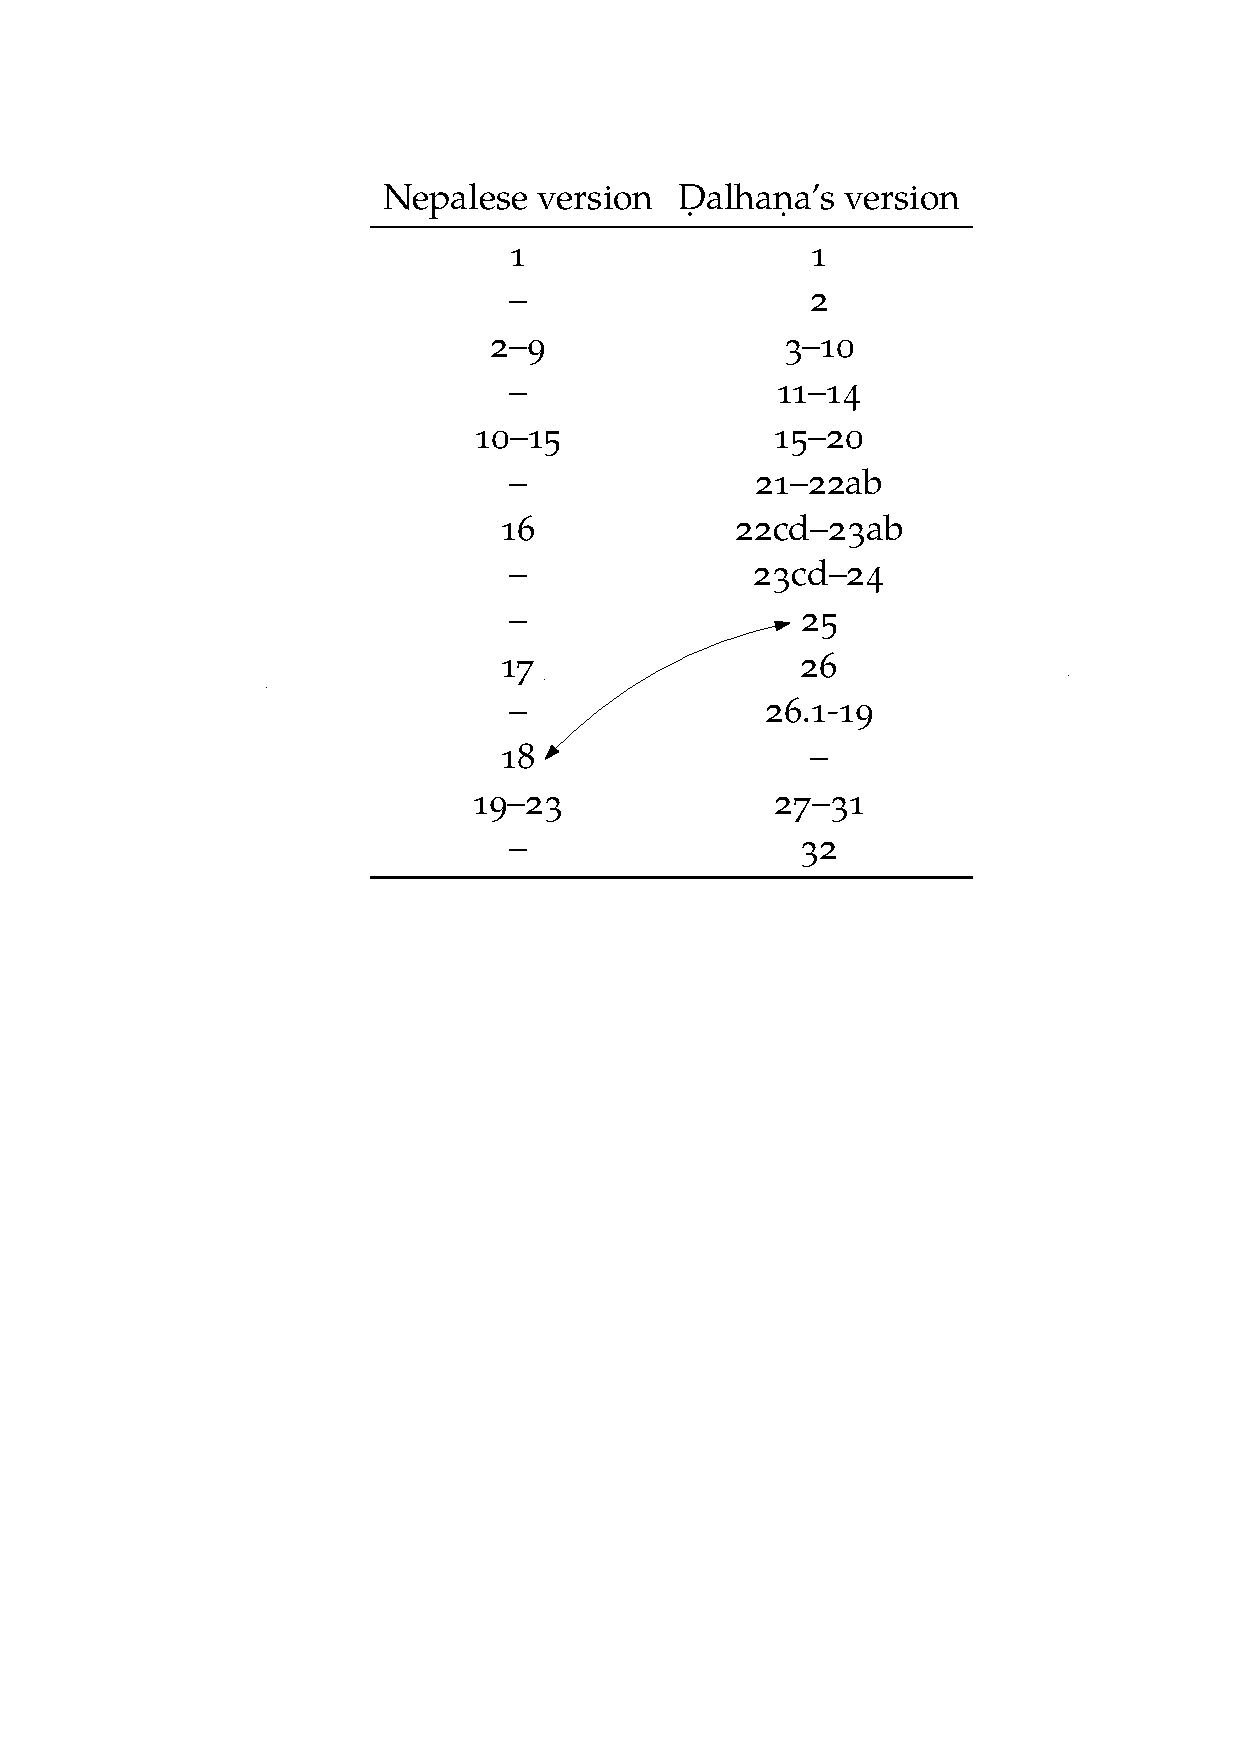
\includegraphics[draft=false,width=\textwidth]{table-of-versions.pdf}
\caption{A Comparison of Verses in 1.16 of the Nepalese and Ḍalhaṇa's Versions}
\end{table}

In Table 1, one can also see that verses 17 and 18 of the Nepalese version were transposed in the redaction of Ḍalhaṇa's version, in which they are 26 and 25 respectively. Although this only occurs once in 1.16, such transposing of verses and even their hemistiches is more prevalent in the redaction of other chapters of the \SS.

Apart from the addition of verses, the redacting of the version known to Ḍalhaṇa involved many small, yet sometimes significant, changes that are summarised below. 

\subsubsection{Changing Spelling, Sandhi and Syntax}
In the majority of cases, efforts were made by redactors to standardise, simplify or improve the language of the Nepalese version. Such changes include the standardising of spelling,\footnote{For example, \emph{pattāṅga} (SS.1.16.21) → \emph{pataṅga} (1.16.29, \cite[81]{vulgate}). For more information on this, see the relevant footnote to the translation.} sandhi,\footnote{or example, \emph{°hastena ṛju} (SS.1.16.2) → \emph{°hastena rju} (1.16.3, \cite[76]{vulgate}).} and verbal forms,\footnote{For example, \emph{unnāmayitvā} (SS.1.16.21) → \emph{prānnamya} (1.16.29, \cite[81]{vulgate}); \emph{avacūrṇayīta} (SS.1.16.21) → \emph{upaharet} (1.16.29, \cite[81]{vulgate}).} as well as interventions to simplify and clarify syntax,\footnote{For example, \emph{śoṇitabahutvanivedanāyāṃ cānyadeśaviddham iti jānīyāt | nirupadravatā taddeśaviddhaliṅgam |} (SS.1.16.3) → \emph{śoṇitabahutvena vedanayā cānyadeśaviddham iti jānīyāt | nirupadravatayā taddeśaviddham iti |} (1.16.4, \cite[76]{vulgate}); \emph{āmatailapariṣekeṇopacaret} (SS.1.16.6) → \emph{āmatailena pariṣecayet} (1.16.7, \cite[77]{vulgate}); \emph{suparigṛhītaṃ} (SS.1.16.10) → \emph{suparigṛhītaṃ ca kṛtvā} (1.16.15, \cite[78]{vulgate}); \emph{anena} (SS.1.16.15) → \emph{snehenaitena} (1.16.20, \cite[79]{vulgate}).} which often involved splitting compounds.\footnote{For example, \emph{yadṛcchāviddhāyāṃ sirāyām} (SS.1.16.4) → \emph{yadṛcchayā viddhāsu sirāsu} (1.16.5, \cite[76]{vulgate}); \emph{dhānyāmlakapālacūrṇaṃ} (SS.1.16.10) → \emph{dhānyāmlaṃ kapālacūrṇaṃ} (1.16.20, \cite[78]{vulgate}).} In some instances, these changes improved the grammar,\footnote{For example, \emph{surāmaṇḍakṣīram} (SS.1.16.10) → \emph{surāmaṇḍaṃ kṣīram} (1.16.15, \cite[78]{vulgate}).} or altered the meaning.\footnote{For example, \emph{kṣīṇālpamāṃsaḥ} (SS.1.16.12) → \emph{kṣīṇo 'lpamāṃsaḥ} (1.16.17, \cite[79]{vulgate}).} However, some prefixes of verbal forms,\footnote{For example, \emph{samvarddhitaḥ} (SS.1.16.8) → \emph{vivarddhitaḥ} (1.16.9, \cite[77]{vulgate}); \emph{niveśya} (SS.1.16.10) → \emph{sanniveśya} (1.16.15, \cite[78]{vulgate}); \emph{avabadhya} (SS.1.16.10) → \emph{ca baddhvā} (1.16.15, \cite[78]{vulgate}).} case endings,\footnote{For example, \emph{māse} (SS.1.16.2) → \emph{māsi} (1.16.3, \cite[76]{vulgate}).} and indeclinables were changed for less apparent reasons.\footnote{For example, \emph{api} (SS.1.16.13) → \emph{vā} (1.16.18, \cite[79]{vulgate}); \emph{ca} (SS.1.16.16) → \emph{tu} (1.16.23, \cite[79]{vulgate}); \emph{tu} (SS.1.16.18) → \emph{ca} (1.16.25, \cite[80]{vulgate}).} There is also a tendency to replace uncommon words with generic ones,\footnote{For example, \emph{mrakṣayet} (SS.1.16.15) → \emph{yojayet} (1.16.20, \cite[79]{vulgate}); \emph{nahyet} (SS.1.16.21) → \emph{baddhvā} (1.16.29, \cite[81]{vulgate}).} add indeclinables,\footnote{For example, [absent]  (SS.1.16.6) → \emph{ca} (1.16.7, \cite[77]{vulgate}); [absent] (SS.1.16.10) → \emph{tatra} (1.16.15, \cite[78]{vulgate}); [absent]  (SS.1.16.12) → \emph{api} (1.16.17, \cite[79]{vulgate}).} omit the verb to be at the end of sentences,\footnote{The words \emph{bhavati} or \emph{bhavanti} are omitted four times in Ḍalhaṇa's version (1.16.10 (twice), 1.16.17 and 1.16.18, \cite[77, 79]{vulgate}).}and introduce verses after a prose passage with the phrase \emph{bhavati cātra}.\footnote{For example, [absent] (SS.1.16.11) → \emph{bhavati cātra} (1.16.16, \cite[79]{vulgate}).} 

% Spelling
% 9. nemī → nemi
% 9. yaṣṭī → yaṣṭi
% 9. kākauṣṭhaḥ → kākauṣṭhakaḥ
% 21. pattāṅga → pataṅga *

%Sandhi
% 2 °hastena ṛju  →  °hastena rju (standardise)*

% Standardising and Simplifying Syntax
% 3.  śoṇitabahutvanivedanāyāṃ cānyadeśaviddham iti jānīyāt | nirupadravatā taddeśaviddhaliṅgam || → śoṇitabahutvena vedanayā cānyadeśaviddham iti jānīyāt || nirupadravatayā taddeśaviddham iti ||*
% 6 āmatailapariṣekeṇopacaret → āmatailena pariṣecayet*

% Clarifying syntax
%15 anena → snehenaitena*

% Splitting compounds
% 4. yadṛcchāviddhāyāṃ	sirāyām	 → 	yadṛcchayā viddhāsu	sirāsu (clarifies syntax)*
% 10. surāmaṇḍakṣīram → surāmaṇḍaṃ kṣīram (improves grammar)*
% 10. dhānyāmlakapālacūrṇañ → dhānyāmlaṃ kapālacūrṇañ*
% 12. kṣīṇālpamāṃsaḥ → kṣīṇo 'lpamāṃsaḥ (changes the meaning)*

% Changing verbs and gerunds
% 2. vyadhayet → vidhyete (perhaps, picking up on karnau)
% 6. kurvīta → dadyāt (middle to active) 
% 7. muñcet → kuryāt
% 9. bandhyā bhavanti → sādhyāḥ
% 10. suparigṛhītaṃ → suparigṛhītaṃ ca kṛtvā ( attempt to improve syntax)*
% 10. upapādya → upadhārya
% 10. sandarśya → sandadhyāt | tato (attempt to simplify the sentence)
% 13. chidyeta → chidyate (opt to pres)
% 15. mrakṣayet → yojayet * (replacing less common words with generic ones)
% 21. nahyet → baddhvā*
% 21. unnāmayitvā → prānnamya (standardise)*
%21 avacūrṇayīta → avacūrṇayet (standardise)*

% Omitting bhavati
% Happens a few times; e.g., 1.16.9 (twice), 1.16.12, 1.16.13

% Changing Prefixes
% 8. samvarddhitaḥ → vivarddhitaḥ*
% 10. niveśya → sanniveśya*
% 10. avabadhya → ca baddhvā*
% 15. marditaṃ → unmarditaṃ*
% 21. unnāmayitvā → prānnamya *

% Changing case endings
% 2. māse → māsi (shift from māsa to mās. Can't see a reason)
% 3. śoṇitabahutvanivedanāyāṃ →  śoṇitabahutvena vedanayā (splitting compounds, but locative of circumstance or condition changed to instrumental of reason. latter is clearer, but not much in it)
% 19. viśleṣitāyām atha nāsikāyāṃ → °tāyās tv nāsikāyāḥ

% changing indeclinables
%13 anyathā → ato 'nyathā
% 13 api → vā*
% 15 tataḥ → ataḥ
% 16 ca → tu*
% 18 tu → ca*
% 19 atha → tu
% 23 vai → syāt

% Adding indeclinables
% 10 [absent] → tatra
% 6 [absent] → ca
% 9 [absent] → tu
% 10 [absent] → ca
% 12 [absent] → api
% 14 [absent] → vā

% Omitting indeclinables
% 9 tatra → [absent]
% 9 ca → [absent]

%Adding bhavati cātra before verses.

% Not sure
% 2
% kṛtamaṅgalaṃ svastivācanan → kṛtamaṅgalasvastivācanan (the latter makes better sense, but could have been original, in my opinion, or an attempt to better integrate a gloss that had become part of the text.)
% abhisāntvayamānaḥ → abhisāntvayan (shift from Pres Pass Part to Pres Act Part) % It seems only the latter is correct in the given context. So, it could be just an error in the NV. Emend or Change translation!!! 
% % 10. agropaharaṇīyāt appears to be an error in the NV that needs to be emended.

\subsubsection{Changing Technical Terms}
There is evidence of standardising and altering technical terminology in subsequent versions of the \SS. Two examples of this in SS.1.16 are the terms for \se{bandha}{joins} and \se{vadhra}{a slice of flesh}. The Nepalese version uses three terms for \se{bandha, sandhāna, sandhi}{joining} splits in the ear flaps and the flesh of nose. Redactors of subsequent versions appear to have tried to standardise this terminology by replacing \emph{sandhāna} and \emph{sandhi} with \emph{bandha} in prose passages.\footnote{For example, \emph{pañcadaśasandhānākṛtayaḥ} (SS.1.16.9) → \emph{pañcadaśabandhākṛtayaḥ} (SS.1.16.10, \cite[77]{vulgate}); \emph{daśakarṇasandhivikalpāḥ} (SS.1.16.9) → \emph{karṇabandhavikalpāḥ} (SS.1.16.10, \cite[77]{vulgate})} However, the use of the term \emph{sandhāna} was retained in verses, perhaps because of the metrical challenges of making such a change. Also, the names of joins which incorporate \emph{sandhāna} and \emph{sandhi} remained the same.\footnote{These names are \emph{nemīsandhānaka}, \emph{kapāṭasandhika}, and \emph{ardhakapāṭasandhika} in SS.1.16.9.}

The Nepalese version (SS.1.16.20,23) contains the rather obscure term \emph{vadhra} for the slice of flesh that a surgeon cuts from the cheek in order to construct a new nose. Modern dictionaries define \emph{vadhra} as a leathern strap (\cite[1385]{apte-prac}, \cite[917]{moni-sans}) or a slice of bacon (\cite[917]{moni-sans}),\q{refs} the latter of which is more indicative of its meaning in the Nepalese version. This word was written out of subsequent versions,\footnote{\emph{vadhram} (SS.1.16.20) → \emph{baddham} (SS.1.16.28, \cite[81]{vulgate}) and \emph{tadvadhraśeṣaṃ} (SS.1.16.23) → \emph{tad ardhaśeṣaṃ} (SS.1.16.31, \cite[81]{vulgate}).} and it was not mentioned as an alternative reading by either Cakrapāṇidatta or Ḍalhaṇa, which suggests that its use and meaning may not have been known to them. However, \emph{vadhra} was used by the author of the \emph{Aṣṭāṅgahṛdayasaṃhitā} (\Ah{Utt.18.62}{841}) in the context of rhinoplasty, so it likely to be the correct reading in the Nepalese version. 

% bandha
% 1. athātaḥ karṇavyadhavidhim vyākhyāsyāmaḥ  → athātaḥ karṇavyadhabandhavidhim adhyāyaṃ (prose)
% sandhāna in all version (verse)
% 9. pañcadaśasandhānākṛtayaḥ (SS.1.16.9) → pañcadaśabandhākṛtayaḥ (SS.1.16.10) (sandhāna is reflected in the name nemisandhānaka, which is in all versions) 
% 9. daśakarṇasandhivikalpāḥ → karṇabandhavikalpāḥ (sandhi is in many of the names, bandha is not)
% 10. (twice) bandha in all versions
% 17 karṇabandha in all versions
% 19 & 23. sandhāna accepted in all versions + 32 in DV. (verse)
% 20. sādhubaddham → sādhubandhaiḥ (verse)
%
% vadhra 
% 20 vadhram → baddham 
% 21 susīvitaṃ → susaṃhitaṃ
% 23 tadvadhraśeṣaṃ → tad ardhaśeṣaṃ

\subsubsection{Augmenting the Text}

Apart from adding whole passages and verses (as seen in Table 1), redactors of subsequent versions augmented the text by expanding existing compounds and inserting new compounds and words. Within the microcosm of 1.16, adjectives and adverbs were inserted to clarify statements,\footnote{For example, \emph{chidre} (SS.1.16.2) → \emph{chidra ādityakarāvabhāsite} (1.16.3, \cite[76]{vulgate}); [absent] (SS.1.16.2) → \emph{śanaiḥ śanaiḥ} (1.16.3, \cite[76]{vulgate});  [absent] (SS.1.16.3) → \emph{āśu} (1.16.5, \cite[77]{vulgate}).} and phrases added to elaborate on diseases and treatments.\footnote{For example, \emph{dhātryaṅke} (SS.1.16.2) → \emph{dhātryaṅke kumāradharāṅke vā} (1.16.3, \cite[76]{vulgate}); [absent] (SS.1.16.2) → \emph{bālakrīḍanakaiḥ pralobhya} (1.16.3, \cite[76]{vulgate});  [absent] (SS.1.16.3) → \emph{picuvartiṃ praveśayet} (1.16.5, \cite[77]{vulgate}).} In particular, the characteristics and number of symptoms of a disease, as well as their reasons for arising, tend to increase in subsequent versions. For example, the Nepalese version (SS.1.16.5) says that the wick in a newly pierced ear should be removed because of aggravated humours or a culpable piercing whereas the version known to Ḍalhaṇa (1.16.6, \cite[77]{vulgate}) includes two further reasons, namely, because of piercing with a painful, crooked and unrecommended needle or because of a wick that is too thick. Some of the split ear flaps in Ḍalhaṇa's version have additional characteristics,\footnote{For example, \emph{pīṭhopamapālir nirvedhimaḥ} (SS.1.16.9) → \emph{pīṭhopamapālir ubhayataḥ kṣīṇaputrikāśrito nirvedhimaḥ} (1.16.10, \cite[77]{vulgate}); \emph{itarālpapāliḥ saṃkṣiptaḥ} (SS.1.16.9) → \emph{utsannapālir itarālpapāliḥ saṃkṣiptaḥ} (1.16.10, \cite[77]{vulgate}); \emph{tanuviṣamapāliḥ} (SS.1.16.9) → \emph{tanuviṣamālpapāliḥ} (1.16.10, \cite[77]{vulgate}).} and a list of four symptoms associated with incurable joins in the Nepalese version (SS.1.16.19) was increased to six in Ḍalhaṇa's version (1.16.10, \cite[77]{vulgate}). Also, models of classifying symptoms were introduced in subsequent versions. For example, the Nepalese version (SS.1.16.4) lists the symptoms of mistakenly piercing a duct in the ear whereas the version known to Ḍalhaṇa (1.16.5, \cite[76–77]{vulgate}) classifies these symptoms according to three ducts called \emph{kālikā}, \emph{marmarikā} and \emph{lohitikā}, which results in some repetition of the symptoms mentioned.\footnote{In Ḍalhaṇa's version  (1.16.5, \cite[76–77]{vulgate}), the symptoms of \se{jvara}{fever} and \se{vedanā}{pain} are repeated. This repetition does not occur in the Nepalese version. It is possible that this classification was not in the version of the \SS\ known to Cakrapāṇidatta (1.16.4, \cite[126]{acar-1939}) because he mentions that some read classifications of ducts at this point in the text and he cites verses from Bhoja on \emph{kālikā}, \emph{marmarikā} and \emph{lohitikā}, but he does not gloss or comment on the passage known to Ḍalhaṇa.}

% Supplementary compounds and phrases for Adding Information
% This is done by expanding compounds, inserting new compounds and adverbs and adding verses and passages.
% 
% 1. karṇavyadhavidhim → karṇavyadhabandhavidhim (foregrounding the term bandha)
% 2
% dhātryaṅke → dhātryaṅke kumāradharāṅke vā (elaborating on treatment)
% upaveśyābhisāntvayamānaḥ → upaveśya bālakrīḍanakaiḥ pralobhyābhisāntvayan (elaborating on treatment)
% chidre → chidra ādityakarāvabhāsite (clarifying technical term)
% [absent] → śanaiḥ śanaiḥ (clarifying treatment)
% [absent] → picuvartiṃ praveśayet (elaborating on treatment)
% 4 
% [absent] →  kālikāmarmarikālohitikāsūpadravā and dividing the adverse affects according to kālikā, marmarikā and lohitikā. Repetition of vedanā and jvara in this process.(discussed in footnote). teṣu yathāsvaṃ pratikurvīt || (adding symptoms, perhaps with a view to managing them more effectively, according to the type of vein pierced).
% 5
% [absent] → kliṣṭajihmāpraśastasūcīvyadhād gāḍhataravartitvād (adding reasons)
% [absent] → yatra saṃrambho vedanā vā bhavati (adding information about the treatment)
%  [absent]  → āśu (clarifies the treatment)
%  [absent] → tāvad yāvat surūḍha iti (until it is well healed - clarifies the treatment)
%9
% pīṭhopamapālir nirvedhimaḥ → pīṭhopamapālir ubhayataḥ kṣīṇaputrikāśrito nirvedhimaḥ (adding characteristics)
% itarālpapāliḥ saṃkṣiptaḥ → utsannapālir itarālpapāliḥ saṃkṣiptaḥ (adding characteristics)
% tanuviṣamapālir → tanuviṣamālpapālir (adding characteristics)
% baddheṣv api dāhapākasrāvaśophayuktā	na siddhim upayānti → tu śophadāharāgapākapiḍakāsrāvayuktā	na siddhim upayānti (adding symptoms)
% 10
% surāmaṇḍodakābhyāṃ → surāmaṇḍoṣṇodakābhyāṃ (adding characteristics of an ingredient)
% 12
% gāḍhapākarāgavān → dāhapākarāgavedanāvān (adding symptoms)

% Additional Verses and Passages (table 1)
% For passages, see subsub on Elaborating on Treatments.
%  [absent] → 16.11–14 (verses)
%  [absent] → 21–22ab, 23cd–24
%  [absent] → 26.1 – 26.19
%  [absent] → 32

\subsubsection{Transposing Words, Verses and Passages}
A close comparison of the Nepalese version with and subsequent ones reveals changes in the order of words, sentences and verses. Examples of such transpositions occur in SS.1.16. In most cases, the changes in word order are insignificant and may be result of different preferences in syntax or even scribal eye-brain-hand miscommunication.\footnote{For example, \emph{aṇusthūla°} (SS.1.16.9) → \emph{sthūlāṇu°} (1.16.10, \cite[77]{vulgate}); \emph{tatraite daśakarṇa°} (SS.1.16.9) → \emph{tatra daśaite karṇa°} (1.16.10, \cite[77]{vulgate}); \emph{nātigāḍhan nātiśithilaṃ sūtreṇāvabadhya} (SS.1.16.9) → \emph{sūtreṇānavagāḍhaman atiśithilaṃ ca baddhvā} (1.16.10, \cite[77]{vulgate}); \emph{pūrvan dakṣiṇaṃ kumārasya vāmaṅ kanyāyāḥ | pratanuṃ sūcyā bahalam ārayā } (SS.1.16.2) → \emph{pratanukaṃ sūcyā bahalam ārayā | pūrvaṃ dakṣiṇaṃ kumārasya vāmaṅ kanyāyāḥ} (1.16.3, \cite[76]{vulgate}).} However, the transposition of verses and passages is usually the result of efforts at redacting the text to add new material. A good example of this is the transposition of Nepalese version's SS.1.16.17 and 18 to Ḍalhaṇa's 1.16.26 and 1.16.25, respectively, which appears to be connected with the insertion of new verses 23cd–24 and 26.1–19 in the latter.

% Words
% 9. aṇusthūla° → sthūlāṇu°
% 9. tatraite daśakarṇa° → tatra daśaite karṇa°
%  10. nātigāḍhan nātiśithilaṃ sūtreṇāvabadhya → sūtreṇānavagāḍhaman atiśithilaṃ ca baddhvā
% Passages
% 2. pūrvan dakṣiṇaṃ kumārasya vāmaṅ kanyāyāḥ | pratanuṃ sūcyā bahalam ārayā || → pratanukaṃ sūcyā bahalam ārayā || pūrvaṃ dakṣiṇaṃ kumārasya vāmaṅ kanyāyāḥ ||
% Verses
%17 and 18 → 26 and 25

%
\subsubsection{Redacting Recipes and Elaborating on Treatments}
Some of the additional text in subsequent versions of the \SS\ supply new ingredients in recipes and procedures in treatments. In many instances, the new material merely clarifies or elaborates on the original but sometimes it changes the recipe or treatment significantly. An example of a suppletion that clarifies the text of the Nepalese version can be seen in 1.16.3 of Ḍalhaṇa's version (\cite[76]{vulgate}), which contains a statement that the physician should insert a wick of cotton after the ear has been pierced.\footnote{For example, [absent] (SS.1.16.2) → \emph{picuvartiṃ praveśayet} (1.16.3, \cite[76]{vulgate}).} This statement anticipates the instructions in the the Nepalese version (SS.1.16.5–6) on removing the wick because of aggravated humours and replacing the wick with a thicker one every three days. In this case, the additional statement of Ḍalhaṇa's version elucidates the role of the wick in the procedure of piercing the ear. 

A similar clarification occurs in 1.16.18 of Ḍalhaṇa's version (\cite[79]{vulgate}), which reiterates the cure for an ear tainted by a humour that was described in 1.16.7 (= SS.1.16.6). The reiteration is quite apt because it follows a passage  (1.16.17, \cite[79]{vulgate} = SS.1.16.12) that outlines the various symptoms of ear disease arising from each of the three humours. The author of Nepalese version probably assumed that, after reading SS.1.16.12, the reader would refer back to SS.1.16.6 for the cure of an ear affected by a humour. However, in Ḍalhaṇa's version, the treatment is reiterated at 1.16.18.

In  Ḍalhaṇa's version of 1.16, there are two instances in which ingredients were added to recipes of medicines in the Nepalese version. The first is the recipe of an anointment that should be applied to a pierced ear that has not healed. In Ḍalhaṇa's version (1.16.7, \cite[77]{vulgate}) the recipe was rewritten to include sesame seeds.\footnote{\emph{yavamadhukamañjiṣṭhāgandharvahastamūlair madhughṛtapragāḍhair ālepayet} (SS.1.16.5) → \emph{madhukairaṇḍamūlamañjiṣṭhāyavatilakalkair madhughṛtapragāḍhair ālepayet} (1.16.7, \cite[77]{vulgate}).} A more significant change occurs in another recipe for an admixture of an oil that is supposed to be rubbed into a healthy ear to enlarge it. Ḍalhaṇa's version (1.16.7, \cite[77]{vulgate}) of the admixture has five additional ingredients, namely, \se{apāmārga}{prickly chaff-flower}, \se{aśvagandhā}{Withania}, \se{kṣīraśuklā}{giant potato}, \se{madhuravarga}{ the `sweet' savour}\footnote{The items which exemplify the `sweet' savour \label{kakolyadi} (\emph{madhuravarga}) are enumerated at SS.1.42.11.} and `milk flower' (\emph{payasyā}  $\rightarrow$ \emph{vidāri}\footnote{Pueraria tuberosa (Willd.) DC. (ADPS 510, IMP 1.792f., AVS 4.391; not Dymock 1.424f. See GJM supplement 444, 451, IMP 1.187, but IMP 3.1719 = Ipmoea mauritiana, Jacq.). }). It also has \se{vidārigandhā}{beggarweed} instead of \se{vidāri}{milk flower}.\footnote{\emph{arkālarkabalātibalānantāvidārīmadhukajalaśūkaprativāpan tailam pācayitvā } (SS.1.16.14) → \emph{arkālarkabalātibalānantāpāmārgāśvagandhāvidārigandhākṣīraśuklājalaśūkamadhuravargapayasyāprativāpaṃ tailam vā pācayitvā} (1.16.19, \cite[79]{vulgate}).} This method of redacting a recipe of Nepalese version appears to be somewhat typical in so far as most of the ingredients of the original were retained and new ones simply added. \q{Perhaps, Dr Madhu could add a comment on whether these additional ingredients would change the effects of the treatment in any significant way?}


% 2. [absent] → picuvartiṃ praveśayet (adding a cotton wick after piercing the ear of a boy or girl)
% 5. yavamadhukamañjiṣṭhāgandharvahastamūlair	madhughṛtapragāḍhair ālepayet → madhukairaṇḍamūlamañjiṣṭhāyavatilakalkair madhughṛtapragāḍhair ālepayet (adding the ingredient tila)
% 5  [absent] → tāvad yāvat surūḍha iti [...] vidhānaṃ tu pūrvoktam eva || (until it is well healed [... One should pierce it again by] the method taught earlier- clarifies the treatment)
% 13.  [absent] → āmatailena trirātraṃ pariṣecayet trirātrāc ca picuṃ parivartayet | (extending the treatment)
% 14. arkālarkabalātibalānantāvidārīmadhukajalaśūkaprativāpan tailam pācayitvā →	arkālarkabalātibalānantāpāmārgāśvagandhāvidārigandhākṣīraśuklājalaśūkamadhuravargapayasyāprativāpaṃ tailam vā	pācayitvā (adding ingredients to an oil)
% additional apāmārga, aśvagandhā, kṣīra, 

 %
\newpage
    \section{The Edition}
    % !TeX root = surgery.tex

\subsection{Manuscripts}
Our edition results from considering the textual evidence of three manuscripts, all of which were preserved and most likely produced in Nepal, in Kathmandu valley, to be more precise. \textcites[\S 
2.1]{kleb-2021b} furnishes a comprehensive description of the individual manuscripts, quotes and translates their colophons and thoroughly examines various problems involved in their interpretation. That is why we will present only the key data essential for the study of our edition in the present paper.
In referring to the manuscripts, we use the sigla K, N and H, which correspond to the initial letters in the names of the libraries and collection where the respective bundles were discovered.

\begin{description}
\item[Siglum K:] The MS has been preserved at the Kaiser Shamsher (KL) library in Kathmandu, accession number KL 699. It was microfilmed and catalogued by the NGMPP/ NGMCP as C 80-7.%
    \footnote{%
    See 
    \url{http://catalogue-old.ngmcp.uni-hamburg.de/mediawiki/index.php/C_80-7_Suśrutasaṃhitā}
     (accessed on October 22, 2021).%
    } 
The MS comprises 152 palm-leaf folios that originally belonged to several different codicological units written by different scribes.%
    \footnote{%
    \textcites[46]{bhat-2020} and \textcites[11]{kleb-2021b} agree that four to five scribes were involved in the manuscript's production.
    } 
The folios are 53.5 $\times$ 4.4 cm in size and have two string holes.  The text is written in the so-called transitional Gupta script, with six to eight lines per folio.%
    \footnote{%
    Codicological features of the manuscript, such as the layout, peculiarities of the script, various ornamental and text-dividing symbols and many more, were scrutinized in \textcites{bhat-2020}.
    }
The MS is incomplete and contains a large part of the \emph{Suśrutasaṃhitā} as well as the \emph{Suśrutanighaṇṭu}.%
    \footnote{%
    See \textcites[11]{kleb-2021b} for a detailed description of the content.%
    }
The date stated in the colophon at the end of the compendium is verified for Sunday, April 13, AD 878. However, some controversy is involved in interpreting the exact roles of two persona mentioned in the same concluding remarks, someone Śrī Harṣacandra and Vaidya Vasuvarman.
\textcites[16]{kleb-2021b} thinks that the former “either sponsored the copying enterprise or wrote the manuscript himself” and that he later “donated it to Vaidya Vasuvarman on the condition that he (Vasuvarman) would study the text and explain it to others. The second condition was that the manuscript should remain in the family and not be given away either for sale or as a pawn. If the manuscript sat unused, it should be returned to Śrī Harṣacandra.”%    
    \footnote{%
    See \textcites[13--17]{kleb-2021b} for a translation and a study of the colophon, as well as an exposition of different positions related to its interpretation.%
    }

\item[Siglum N:] This MS is kept at the National Archives Kathmandu (NAK), under accession number 1-1079 \dev{ka}. It was microfilmed twice by the NGMPP as A 45-5(1) and A 1267-11(2).%
    \footnote{%
See 
\url{http://ngmcp.fdm.uni-hamburg.de/mediawiki/index.php/A_45-5_(Suśrutasaṃhitā)}
 (accessed on October 22, 2021)/
    } 
The MS comprises 65 palm-leaf folios, 56 $\times$ 5 cm in size, with two string holes each, and it is bundled together in a composite manuscript with at least one other medical work. The text is written in a variety of Newari script, with ca.\ seven lines per folio. Although the text contained in the MS does not cover the entire \emph{Suśrutasaṃhitā} and breaks off abruptly in the second chapter of the \emph{śārīrasthāna}, the actual MS, as a codicological unit, appears complete, that is, no leaf seems to be missing from the originally unitary artefact. Based on paleographic considerations, the MS can be dated tentatively to the 12th or 13th century.

\item[Siglum H:] The MS belongs to the historical collection of Hemarāja Śarman (fl.\ 1878-1953) and is currently kept at the NAK under accession number NAK 5-333. It is microfilmed twice by the NGMPP as B 29-19 and B 30-15, but the latter microfilm is incomplete.%
    \footnote{%
    See 
    \url{http://ngmcp.fdm.uni-hamburg.de/mediawiki/index.php/B_29-19_Suśrutasaṃhitā}
     (accessed on October 22, 2022).
    } 
The MS comprises 435 palm-leaf folios, 34 $\times$ 5 cm in size, with one string-hole in the middle. It is written in a type of Newari script that is more recent than the one used in N, with approximately six lines per folio. The MS is exceptionally well-preserved and complete, containing the text of the \emph{Suśrutasaṃhitā} as well as the \emph{Suśrutanighaṇṭu}. The final colophon identifies the scribe of the MS as Vaidya Amarasiṃhaka, son of Kamaladatta, and states the date on which he concluded the copying of the text. Both reading, that is, deciphering the actual characters, and interpretation of the concerned passage involve diverging opinions, all of which concur, however, in assigning the MS to the 16th century. \textcites[21--26]{kleb-2021b} gives an analytical account of the views expressed in literature, considers further options and puts forward his understanding that the MS was completed on Sunday, July 29, AD 1543.  
\end{description}
  
\subsubsection{Features of the manuscript transmission}
Andrey
\subsubsection{Palaeographical features}
\begin{itemize}
    \item śrita for śṛta.
    \item yātri for yātṛ (Su.ka.1.63) % but yātrin is possible
     \item punarṇṇavā  (Su.ka.1.61) % but an old Nepelase ms. of the Brahmayāmala has this spelling.
    \item ś and s in KL 699.
    \item b and v in KL 699 and NAK 5-333.
    \item cha and ccha
    \item line-fillers
    \item \d n for n (punar\d n\d nav\=a)
    \item vyājī-kṛ for vājī-kṛ
\end{itemize}

\subsubsection{Chart of characters}

[[[Put a chart from QuickPalaeographer here.]]]

\subsection{The Printed Editions}

The careful survey of printed editions of the \SS\ by Meulenbeld lists no fewer than 
44 entries.\footcite[IIB, 311--314]{meul-hist}  These range from the first edition 
by 
Madhusūdana Gupta (\citeyear{gupt-1835}) to editions in the 1970s. The 
number of 
reprints and editions since that time might almost double that number.  
Translations begin with Hessler's Latin translation in \citeyear{hess-1855} and 
continue up to the present in scores of publications in many 
languages.\footcites[E.g.,]{zysk-1984}[IIB, 314--315]{meul-hist}

\subsubsection{The Vulgate}


The great ayurvedic scholar Yādavaśarman Trivikrama Ācārya produced three 
successive editions of the
\SS\ with the commentary of Ḍalhaṇa, in 1915, 1931 and 1938.  These
editions, especially the last, are generally considered the most 
scholarly
and reliable editions of the work, and have been constantly reprinted up
to the present day.\footnote{See also the study of these editions by \textcites[\S 
1.2]{kleb-2021b}[143--144]{wuja-2013}.}  We refer to the last of these editions 
as “the vulgate.”

The 1915 edition was based on three manuscripts.  The 1931 edition used another
seven manuscripts plus two printed editions.  For his final 1938 edition, Ācārya
used a further three manuscripts.\footnote{The following account of the sources is
paraphrased from \citeauthor{vulgate}'s own account of his sources
\citep[22]{vulgate}.}  These sources are described as follow, with an overview in
Table~\ref{tableofeds}.

\subsubsection{The sources of the 1915 edition}

\begin{enumerate}
    \item[1] Calcutta, Royal Asiatic Society.  Covers the \emph{sūtra, nidāna, śārīra 
    and 
        kalpa sthāna}s.  
    
    \item [2] Jaipur, Pandit Gaṅgādharabhaṭṭaśarman, lecturer at the Royal 
    Sanskrit University.  Covers the \emph{cikitsāsthāna} and the 
    \emph{uttaratantra}.
    
    \item [3]  Bundi, my great friend the royal physician Paṃ.\ Śrīprasādaśarman  
    Covers the \emph{uttaratantra}.
\end{enumerate}

\subsubsection{The sources of the 1931 edition}

\begin{enumerate}
    
    \item[1] Vārāṇasī, professor of literature, the great Gaurīnāthapāṭhaka.  With 
    the 
    \emph{Nibandhasaṅgraha}. Covers the \emph{nidānasthāna} and 
    \emph{uttaratantra}.
    
    \item [2]  Ahmedabad.  My friend Sva.\ Vā.\ Vaidya Raṇachoḍalāla 
    Motīlālaśarman.  
    With the \emph{Nibandhasaṅgraha}.  Covers the \emph{śārīrasthāna}.
    
    \item [3] From the personal library of my great friend Sva.\ Vā.\ Vaidya
    Murārajīśarman. Extremely old. No commentary.  Covers the 
    \emph{śārīrasthāna}.
    
    \item [4]  Puṇe, BORI library.  With the \emph{Nibandhasaṅgraha}. Covers the
    \emph{śārīrasthāna}.\footnote{Not one of the three MSS of the
    \emph{śārīrasthāna} described in \cite{shar-vaid}.}
    
    \item [5]  Puṇe, BORI library.  With the \emph{Nibandhasaṅgraha}. Complete.  
    With some damaged folia.
    
    \item [6]  Bombay, Asiatic Society.  Incomplete.\footnote{Possibly 
    \MScite{Mumbai 
    AS B.I.3} or \MScite{Mumbai AS B.D.109} \citep[v.\,1, \# 212 and 
    213]{vela-1930}.  But both these have the \emph{Nibandhasaṅgraha}.  The 
    first 
    covers only the \emph{śārīrasthāna}; the second may be complete, but 
    Velankar calls it 
    only “disorderly.”}
    
    \item [7] Varanasi, the private library of Vaidya Tryambakaśāstrī.  Covers the 
    \emph{cikitsāsthāna}.  The variant readings of this MS were compiled by Prof.\ 
    %    Guruprasādaśāstrī and supplied to Ācārya.
    
    \item [8]  A printed edition together with the commentary 
    \emph{Suśrutasandīpanabhāṣya} by Professor Hārāṇacandra Cakravārtti. 
    Complete work.
    This is the 1910 Calcutta edition numbered “t” by \citet[IB, 
    312]{meul-hist}.\footcite{bhat-1917}
    
    \item [9] A printed edition of the first 43 chapters of the
    \emph{sūtrasthāna}, printed in Bengali script, with the commentaries
    \emph{Bhānumatī}, \emph{Nibandhasaṅgraha}, edited by Vijayaratnasena and
    Niśikāntasena. This is the 1886 Calcutta edition numbered “g” by \citet[IB,
    311]{meul-hist}.\footcite{sena-1886}
    
\end{enumerate}

%
\begin{table}
    \caption{The sources of Yādavaśarman T. 
        Ācārya's 
        three editions:\\ manuscript coverage (\newmoon) and print coverage
        ($\circ$). \label{tableofeds}}
    \vspace{.5\baselineskip}
    
    \begin{tabular}{c|ccc|ccccccccc|ccc}
        \toprule
        %        \multicolumn{16}{c}{\emph{Manuscripts (\newmoon) and print 
        %editions 
        %                ($\circ$)}} \\
        \emph{edition}            &\multicolumn{3}{c}{1915}
        &                \multicolumn{9}{c}{1931} 
        &              \multicolumn{3}{c}{1938} \\
        
        \emph{source}         & 1 & 2 & 3 & 1 &2  &3  &4  &5  &6  &7  &8  &9  &1  
        &2 &3 \\
        
        
        \midrule
        
        \emph{sthāna} &&&&&&&&&&&&&&&\\        
        
        \emph{sū}. &  \newmoon&  &  &
        &  &  &  & \newmoon & ? &  & $\circ$ & 
        $\circ$\footnotemark &  
        \newmoon & &\newmoon \\
        
        \emph{ni}. &\newmoon  &  &  &
        \newmoon &  &  &  &  \newmoon&  ?&  & $\circ$ &  &  
        \newmoon&\newmoon & \newmoon\\
        
        \emph{śā}. &  \newmoon&  &  &
        & \newmoon & \newmoon & \newmoon & \newmoon &  ? &  &  
        $\circ$&  &  
        \newmoon& &\newmoon \\
        
        \emph{ci}. &  & \newmoon &  &
        &  &  &  &\newmoon & ? &  \newmoon&$\circ$  &  &
        \newmoon & &\newmoon\footnotemark \\
        
        \emph{ka}.  &\newmoon  &  &  &
        &  &  &  &\newmoon  &  ?&  & $\circ$ &  &  
        \newmoon  & & \\
        
        \emph{utt}.  &  & \newmoon &\newmoon  &
        \newmoon  &  &  &  & \newmoon & ? &  & $\circ$ &  &  
        & & \\
        \bottomrule
    \end{tabular}
\end{table}  
\addtocounter{footnote}{-1}
\footnotetext{Covers chapters 1--43 only.}
\stepcounter{footnote}
\footnotetext{Covers chapters 1--9 only.}
%
\subsubsection{The sources of the 1938 edition}
% \coffeestainC{1}{1}{180}{0}{-5 mm}
\begin{enumerate}
    \item [1]  Gwalior, from the library of my great friend Paṃ.\ Rāmeśvaraśāstrin 
    Śukla. 
    Covers the \emph{sūtra, nidāna, śārīra, cikitsā and kalpasthāna}s.
    
   \item[2] Bikaner, from the library of the Royal Palace, supplied by Paṃ.\ 
Candraśekharaśāstrin. Contains the commentary 
\emph{Nyāyacandrikāpañjikāvyākhyā} by Gayadāsa.  Covers the 
\emph{nidānasthāna}.  

This is almost certainly \MScite{Bikaner Anup 
    4390}.\footnote{See Dominik Wujastyk, “MS Bīkāner AnupLib 4390.” 
\emph{Pandit}. 
<\url{http://panditproject.org/entity/108068/manuscript}>.}

\item [3] Kathmandu, located in the private library of the Royal Guru Hemarāja 
Śarman.  An extremely old palm-leaf manuscript. Readings from this MS were 
compiled by Paṃ Nityānandaśarman Jośī and sent to Ācārya. Covers from the 
beginning of the work to the end of the ninth chapter of the 
\emph{cikitsāsthāna}.  The 
siglum for this manuscript in footnotes was \dev{tā} for 
\dev{tālapatrapustake}. 
\end{enumerate}
\subsubsection{Evaluation}

Estimates show that there are approximately 230 extant manuscript
witnesses for the \emph{Suśrutasaṃhitā}.\footnote{This figure is arrived
at by summing the MSS mentioned in \cite{ncc} and in the \cite{ngmcp}. The
real figure could be many scores higher.}  Many of these manuscripts cover only
one or more or its chapters.  Nevertheless, this is an order of magnitude
more evidence than was considered by Ācārya for his vulgate editions.

While the descriptions provided by Ācārya of his source materials seems at first
to be moderately comprehensive, Table~\ref{tableofeds} reveals the underlying
paucity of textual sources for these editions.  At first, it appears that fifteen
manuscripts were consulted.  However, we quickly see that two of the sources 
were
other people's printed editions, and one of those covered less than a quarter of
the work (no.\,9 of 1931).  That reduces the manuscript base to 13 manuscripts.
Ācārya does not appear to have seen two of the manuscripts at all, having been
sent collations prepared for him by others (7 of 1931 and 3 of 1938).  Thus,
Ācārya's final edition was based on the personal consultation of eleven partial
manuscripts.   One of them remains unidentified (6 of 1931). Only a single
manuscript covers the whole of the \emph{Suśrutasaṃhitā}, no.\,5 of the 1931
edition.  Manuscript 1 of 1938 is the next most complete, but it omits the
\emph{uttaratantra}, which comprises a third of the work.  Manuscript 1 of the
1915 edition is third in size, but it still omits both of the longest chapters,
and thus offers less than half the work.  For the rest, the evidence is spotty,
with each part of the work being supported by only between four and eight
manuscripts, excluding the printed editions.

Two sources stand out for their historical importance.  The first is no.\,3 of
1931, which Ācārya calls “extremely old.”  It covered the \emph{śārīrasthāna}
only, and unfortunately we know nothing of the later history of this manuscript.
The second is no.\,3 of 1938, which is one of the important Nepalese manuscripts
being considered in the present project. Ācārya's remarks and references to
Hemarājaśarman's introduction to the \emph{Kāśyapasaṃhitā} allow us
to identify this manuscript as \MScite{Kathmandu NAK 
    5-333}.\footnote{\cites[22]{vulgate}[56--57]{hema-1938}. Discussed by
\citet[\S 1.1, 2.3]{kleb-2021b}.  See also \cites[IIB, 
25--41]{meul-hist}[161--169]{wuja-2003}.} But 
that manuscript covers the whole work, not
just up to the ninth chapter of the \emph{cikitsāsthāna} as
\citeauthor{vulgate} stated.\footcite[22]{vulgate}  Perhaps the editors
only received collations for this portion of the manuscript and did not know that it
was a witness for the whole work.

\subsubsection{The 1939 edition}        

In 1939, Yādavaśarman Trivikrama Ācārya and Nandakiśora Śarman co-edited an
edition of the \emph{sūtrasthāna} of the \emph{Suśrutasaṃhitā} that was 
published
by the Swami Laxmi Ram ayurvedic centre in Jaipur, and printed at the famous
Nirṇayasāgara Press in Mumbai (see 
Fig.\,\ref{bhanumati}).\footnote{\cite{acar-1939}.  The description of 
the sources 
below is based on Yādavaśarman T. Ācārya's  remarks in his introduction 
(pp.\,3--4). See also the remarks on this edition by
\citet[7]{kleb-2021a}.  On the Swami Laxmi Ram
centre, see \cite{hofe-2007}} The text was edited on the basis of the following 
sources.

\begin{figure}[p]
    \centering
    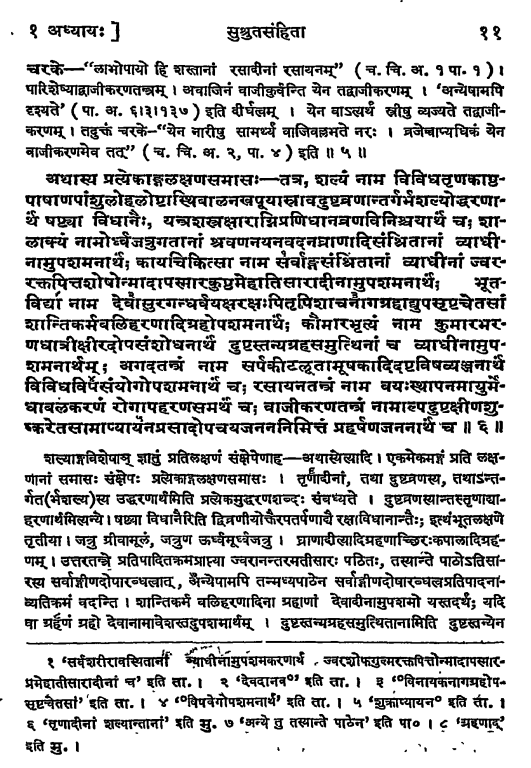
\includegraphics[draft=false,height=.9\textheight]{media/Bhanumati-page-11}
    \caption{A page of the 1939 \emph{Bhānumatī} edition, showing the variant 
        readings in 
        the 
        footnotes.}
    \label{bhanumati}
\end{figure}


\paragraph{For the Bhānumatī}

\begin{enumerate}
    \item A printed edition.  Covered the \emph{Bhānumatī} up to chapter Su.sū.40.
    The siglum was \dev{mu} for \emph{mudrita}.\footnote{\cite{sena-1886}.  
    The
    manuscript on which this edition was based is probably in the library of the
    Calcutta Sanskrit College, and described in \cite[v.\,X.1]{sast-1917}, which
    is not available to me.  See also \cite[IB, 495, n.\,57]{meul-hist} for
    mention of this manuscript.  The reference at \cite[217]{rao-sans} to CSCL
    accession number 97 in Bengali script may be this manuscript.}
    
    \item A manuscript in the India Office Library library provided through the
    Bhandarkar Oriental Research Institute in Pune.\footnote{At this time,
    manuscripts from Britain were routinely lent to scholars in India and vice
    versa.} This manuscript covered the \emph{Bhānumatī} b up to the end of the
    \emph{sūtrasthāna}.  The siglum was \dev{ha} for
    \dev{hastalikhita}.\footnote{\cite{PP109978}\\ 
    \MScite{London BL H. T. Colebrooke 908}
    (\href{panditproject.org/entity/109978/manuscript}{PanditProject \#109978},
    consulted on July 03, 2021).}
\end{enumerate}

\paragraph{For the Suśrutasaṃhitā}

\begin{enumerate}
    \item A palm leaf manuscript from Hemarājaśarman's personal
    library.\footnote{I.e., \MScite{Kathmandu NAK 5-333}.}  The siglum was
    \dev{tā} for \dev{tāḍapatra}.
    
    \item His own published edition. The siglum was \dev{ḍa} for 
    \dev{ḍalhaṇasaṃmataḥ
        pāṭhaḥ}.\footnote{\cite{vulgate}.  It is noteworthy that Ācārya refers to
    his 1938 edition as representing “the Ḍalhaṇa recension.”}
    
    \item Hārāṇacandra Cakravarti's published edition with his own
    commentary.\footcite{bhat-1917} The siglum was \dev{hā}.
\end{enumerate}
%
\subsubsection{Evaluation}

The main innovation of this publication was to present the only surviving part of
the commentary on the \SS\ by the great eleventh-century medical scholar
Cakrapāṇidatta, namely the \emph{Bhānumatī}.\footcite[IA, 374--375 and IB,
495--496]{meul-hist} A secondary purpose was to present the text of the
\emph{sūtrasthāna} as read in \MScite{Kathmandu NAK 5-333}, that had recently 
been
brought to the editors' attention. In their judgement, the Kathmandu manuscript
presented a text that was closer to what Cakrapāṇidatta had before him than the
text according to Ḍalhaṇa.   This was the first \SS\ edition in which Ācārya used
sigla to identify the sources from which variant readings were reported, so while
it has limitations, it for the first time enables us to get some idea of origins
of the text (see Figure~\ref{bhanumati}).

Ācārya noted in his introduction that the manuscripts containing the Ḍalhaṇa's
commentary all came together with the root-text of the \SS, and thus the main \SS\
text reflected the readings chosen by Ḍalhaṇa.  But the manuscripts of the
\emph{Bhānumatī} contained the commentary alone, without the root-text, and 
had
many explanations based on different readings of the root-text than those of
Ḍalhaṇa.  In many of these cases it was hard to know what the text that
Cakrapāṇidatta had before him. But Ācārya noted that Cakrapāṇidatta had a text
before him that had much in common with the text of the Nepalese
manuscript.\footnote{\cite[3--4]{acar-1939}.  See discussion by
\citet[7]{kleb-2021a}.}  

There is compelling evidence that Cakrapāṇidattas's \emph{Bhānumatī} 
commentary
once covered the whole text of the \SS.\footcite[IA, 375]{meul-hist}  The loss of
the rest of the work ranks amongst the greatest disasters in Āyurvedic
literature.  Remarkably, the whole \emph{Bhānumatī} may still have existed in the
early twentieth century. In 1903, Palmyr Cordier reported being privately informed
of a complete copy of the work in a personal manuscript collection in
Benares.\footcite[332]{cord-1903}
   
\subsection{Editorial Principles}
\subsubsection{Method}
The data for the critical edition comes from the witnesses of the Nepalese version, which are MS KL 699, NAK 5-333 and NAK 1-1079. Diplomatic transcriptions of SS.1.16 of these manuscripts have been created by researchers of the \href{https://sushrutaproject.org}{Suśruta Project}\space%\footnote{https://sushrutaproject.org, accessed 20/8/2021.} 
according to a subset of TEI Guidelines that has been formulated by Charles Li.\footnote{These guidelines are at \url{https://saktumiva.org/wiki/tei}, accessed 20/10/2021.} MS NAK 5-333 was transcribed first because its script is easy to read, the scans are clear, and it is the most complete of the manuscript witnesses. Then, MS KL 699 and MS NAK 1-1079 were transcribed. 

The diplomatic transcripts were uploaded to Charles Li's platform Saktumiva, which automatically collates them. An electronic text of the vulgate of the \SS, which was transcribed without the commentaries by Tsutomu Yamashita and Yasutaka Muroya on the basis of Ācārya's 1931 and 1938 Bombay editions,\footnote{This e-text is available on the SARIT website; \url{https://sarit.indology.info/susrutasamhita.xml?view=div}, accessed 20/8/2021.} has also been included in the collation. 

Saktumiva's automatic collation function standardises punctuation and orthographic variants according to filters which can be turned off or on. These filters enable the editors to ignore \emph{daṇḍa}s, numbers and \emph{puṣpikā}s in the transcripts, as well as orthographic variants, such as \emph{ba} and \emph{va}, certain germinated consonants, and \emph{visarga} variants. On the basis of the automatic collation, Jason Birch created a provisional edition of SS.1.16, which the project's researchers read together at weekly seminars. Manuscript images were routinely checked to verify the transcripts, particularly when a reading was uncertain; the commentaries of Cakrapāṇidatta and Ḍalhaṇa were read, and variant readings reported by these commentators were included in notes to the edition. Also, various reference books were consulted, such as the  \citet{josi-maha,nadk-1954} and \citet{meul-hist}, to elucidate the meaning of technical terms and identify relevant information in other medical works. 

An initial draft of the translation and many annotations were written by Dominic Wujastyk during the seminars as the Project researchers discussed the text's meaning. The transcripts, provisional edition and translation were uploaded to the project's repository at Github on a weekly basis. Therefore, the project's work has been publicly available as it evolves. The following software tools have been selected by Wujastyk for the procedures described above: 

\begin{enumerate}
    \item
    \href{https://www.oxygenxml.com.}{oXygen XML editor} (which has plugins for Github and TEI, and can validate the code).%\footnote{https://www.oxygenxml.com.}
    
       \item
        \href{http://saktumiva.org.}{Saktumiva} (a platform for producing and publishing critical editions of Sanskrit texts).%\footnote{http://saktumiva.org.}
        \item
         \href{https://tst.hypotheses.org/1738.}{Quick Palaeographer} (a browser-based tool for reading MS images and developing a catalogue of character shapes).%\footnote{https://tst.hypotheses.org/1738.}

        \item
         \href{https://filezilla-project.org.}{Filezilla} (document transfer to Saktumiva).%\footnote{https://filezilla-project.org.}       
        \item
         \href{https://github.com.}{Github} (document sharing, security and versioning).%\footnote{https://github.com.}   
        \item
          \href{https://www.latex-project.org.}{LaTeX} (document preparation).%\footnote{https://www.latex-project.org.}  
         \item
           \href{https://qdpm.net.}{qdpm} (project management).%\footnote{https://qdpm.net.}  
          
\end{enumerate}

\subsubsection{Stemma}
The data from transcripts collated by Saktumiva can be exported as a FASTA file 
and aligned according to characters, syllables or words by a program called 
Helayo. The resulting NEXUS file can be read by phylogenetics software to build a 
stemmatic tree.\footnote{This process is discussed in greater detail by Charles Li 
at \url{https://chchch.github.io/sanskrit-alignment/docs/index.html\#tree}, 
accessed 21/8/2021.} This procedure was done with transcripts of several 
chapters of the Nepalese witnesses, and the results confirmed the editors' provisional stemmatic hypothesis that 
K and H are more closely related to one another than K and N.\footnote{See 
section `Features of the Manuscript Transmission' for further discussion of this.} 
Given the early date of K and the small number of other surviving witnesses of the 
Nepalese version, the relationship between the manuscripts at our disposal is 
reasonably clear and, in the case of SS.1.16, the manuscript data was largely 
confined to N and H owing to a missing folio of K. The challenge of editing has 
been to repair the text in the places where it has become corrupt in the
available witnesses. 

\subsubsection{The Edition and Apparatus}
The critical edition of SS.1.16 in this article retains many of the peculiarities of MS KL 699 because the editors have endeavoured to present to the reader a text that is very similar to the one transmitted in the region of Nepal in the ninth century. Therefore, the Sanskrit has been standardised as minimally as possible and, although the text has been corrected and repaired wherever it seemed corrupt, it has not been normalized or conventionalized to the extent of many modern editions of Sanskrit works. 

The editors have assumed that the authors of the Nepalese \SS\ were familiar with Pāṇinian Sanskrit and, although there are some non-standard spellings and grammatical forms in the text, there are very few instances of hyper-Sanskritization, Buddhist-hybrid Sanskrit or Epic forms that would suggest that this assumption is unreasonable. Therefore, the editors of SS.1.16 have opted to retain some unusual features of the Sanskrit in MS KL 699 when they are grammatically correct. For example, in external \emph{sandhi}, the class nasal is usually used at the end of a word instead of an \emph{anusvāra} (e.g.,1.16.3, \emph{°vācanan dhātry°}), although the \emph{anusvāra} is sometimes used (1.16.15, \emph{udakaṃ dhānyāmla°}). In most cases, the consonant following a \emph{repha} is doubled, but this is not always the case.\footnote{Examples of the germination of consonants are \emph{karṇṇa} (1.16.1 ff), \emph{muhūrtta} (1.16.2), \emph{pūrvva} (1.16.2), \emph{gandharvva} (1.16.5), \emph{°mūlair mmadhu°} (1.16.5), \emph{vartti} (1.16.6) and \emph{punar vvidhyet} (1.16.6). Examples where it does not occur in 1.16 are  \emph{°ārtham} (1.16.8,19), \emph{kuryāt} (1.16.16, 32), \emph{°pālir vallūra°} (1.16.10); \emph{°pālir vyāyojimaḥ} (1.16.10) and \emph{dīrghaika°} (1.16.10).} Since these inconsistencies seem inherent to the transmission of the text and may have even been authorial, the critical edition reflects them as they occur in K and, when the testimony of K is not available, the witness most similar to K, which is H.


% This is not always consistent: °ārtham (1.16.8,19), kuryāt (1.16.16, 32), °pālir vallūra°  (1.16.10); °pālir vyāyojimaḥ (1.16.10); dīrghaika° (1.16.10).

% external sandhi
% A tendency to favour the use of the class nasal instead of ṃ (e.g.,1.16.3 svastivācanan dhātryaṅke), although ṃ is sometimes used (1.16.15 udakaṃ dhānyāmla°)

% germination of consonants after a repha, even between words.
% karṇṇa (1.16.1 ff), muhūrtta (1.16.2), pūrvva (1.16.2), gandharvva (1.16.5), °mūlair mmadhu° (1.16.5), vartti (1.16.6), punar vvidhyet (1.16.6), °pālir nnirvvedhimaḥ
% This is not always consistent: °ārtham (1.16.8,19), kuryāt (1.16.16, 32), °pālir vallūra°  (1.16.10); °pālir vyāyojimaḥ (1.16.10); dīrghaika° (1.16.10).

The Nepalese manuscripts often have an \emph{anusvāra} before a \emph{daṇḍa} at the end of a sentence or verse. Whether these \emph{anusvāra}s should be changed to the consonant \emph{m} is a moot question because there is no Pāṇinian concept of `end-of-sentence' and his rules on \emph{sandhi} are contingent on the close contact of  sounds (\emph{saṃhitā})\q{refs?}. However, it is reasonable to assume that at the end of a verse, paragraph or sentence the speakers would have paused for breath or thought, in which case \emph{sandhi} should be applied and a final \emph{anusvāra} or class nasal of the following consonant changed to \emph{m}.  Nonetheless, this remains an assumption about how the text would be pronounced. Therefore, the insertion of \emph{daṇḍa}s and changing \emph{anusvāra}s to \emph{m} before them in the critical edition are subjective decisions by the editors. The scribal use of \emph{daṇḍa}s and \emph{anusvāra}s in the Nepalese manuscripts can be seen in the digital edition if one switches off the filters for ignoring \emph{daṇḍa}s and final \emph{anusvāra} variants. 

Unconventional spellings and grammatical forms have been retained and noted in the annotations to the translation. However, the editors have corrected scribal errors and repaired corruptions in the transmitted text with conjectures wherever possible. Therefore, although the edition retains many of the peculiarities of the Nepalese manuscripts, it is not a diplomatic transcript or a hybrid of diplomatic and critical editing because the features of the transmitted text have been retained or changed deliberately, and the reasons for doing so are given in either the introduction or, in more specific cases, the annotations to the translation.

\subsubsection{Printed Edition}
The apparatus of the critical edition in this article is positive, that is to say, the testimony of every witness is recorded for the lemma and variants. This samply entry should be interpreted as follows:
\begin{quote}
pratanuṃ K ]  pratanū N, H tataḥ A\\
The chosen reading pratanuṃ is the reading of K. The witnesses N and H have pratanū and A has tataḥ.
\end{quote}
Conjectures by the editors are indicated by the abbreviation \emph{conj}. Omissions and suppletions in the witnesses are represented by \textsc{[OM]} and \textsc{[ADD]} next to the siglum. There are separate layers of footnotes in the printed edition for testimonia and notes. The testimonia usually consist of the variant readings noted by the commentators Cakrapāṇidatta and Ḍalhaṇa. The notes include the additional passages and verses in the version known to Ḍalhaṇa and large omissions in the witnesses.

\subsubsection{Digital Edition}
The apparatus of the digital edition is negative in so far as the lemma and its witnesses are not included. However, a positive apparatus is available in the digital edition if one highlights one or more words, and even entire passages or verses, and clicks on the collapsed menu icon. 




 %
\newpage
    \section{The Translation}
    % !TeX root = surgery.tex

% turn off the footnotes, for the conference handout
%\renewcommand\footnote[1]{\relax }



%INTRODUCTION
%A. Preliminaries
%1. Aim of the Article
%2. Importance of 1.16 in the History of Āyurveda 
%B. Text
%1. The Nepalese Version
%2. Vulgate
%3. Differences between the Two (as exemplified by 1.16)
%C. Edition 
%1. Manuscripts
%2. Editorial Principles
%EDITION OF 1.16 

  \newcommand{\animal}[4]{#1 (\emph{#2}%\footnote{#3 (#4)})
}
\newcommand{\plant}[4]{#1 (\emph{#2}%\footnote{#3 (#4)})
}
\newcommand\skt[2]{#1 (#2)}


 \section{Translation of Sūtrasthāna 16}
%\subsection{Sūtrasthāna, adhyāya 16}

\begin{translation}    
  
\item [1] 

Now we shall expound the method for piercing the ear.\footnote{The topic of 
    \se{kaṛnavyadha}{piercing the ear} is not discussed in the \emph{Carakasaṃhitā}
    (\cite[IB, 326, n.\,175]{meul-hist}), but it is mentioned in some texts that
    followed the \emph{Suśrutasaṃhitā}, such as the \emph{Kaśāpyasaṃhitā} \citep[IIA,
    30]{meul-hist}. Also, the instrument for piercing the ear is described in the
    \emph{Aṣṭāṅgahṛdayasaṃhitā} \Ah{1.26.26}{321}. In the versions of the text known
    to Ḍalhaṇa \citep[76]{vulgate} and Cakrapāṇidatta \citep[125]{acar-1939}, the
    heading of this chapter is “the method of piercing and joining the ear”
    (\emph{karṇavyadhabandhavidhi}), instead of the Nepalese version's “the method of
    piercing the ear” (\emph{karṇavyadhavidhi}). The topic of joining the ear
    (\emph{karṇabandha}) is discussed in passages 17--20 of the Nepalese version.
    However, it appears that only subsequent redactors reflected its importance by
    including it in chapter headings.

 The Nepalese version also omits the opening remark on Dhanvantari that appears in
subsequent versions of the text. For a discussion of the frame story in the
Nepalese version, see \cite{birc-2021}. Ḍalhaṇa \citep[76]{vulgate} and
Cakrapāṇidatta \citep[125]{acar-1939} state that only the ears of healthy people
should be pierced, and they quote the lost authority Bhoja to affirm this: “When
piercing the ears of children who are free of disease at these times, their ear
flaps and apertures, as well as limbs, increase” (for the Sanskrit, see
\cite[76]{vulgate}).

Some texts use the adjective \emph{karṇavedhanī} rather than\emph{-vyadh-}.}

\item [2] 

One may pierce a child's ears for the purpose of preserving and decorating. On
renowned days, half days, hours and constellations the physician, with a calming presence, 
sits the
boy, who has received a benediction and the recitation of a blessing,\footnote{The
    causative form \emph{vy\u adhayet} is known in Classical Sanskrit
    \citep[166]{whit-root}.

The compound \emph{kṛtamaṅgalasvastivācanaṃ} “who has received a benediction and
the recitation of a blessing” is an emendation based on the similar text at
\Su{3.2.25}{346}.  Cf.\ also \Su{3.10.8, 24}{388, 390} that have slightly
different formulations.} on the lap of a wet-nurse.\footnote{The versions of
    1.16.3 known to Cakrapāṇidatta \citep[126]{acar-1939} and Ḍalhaṇa
    \citep[76]{vulgate} have the additional compound \emph{kumāradharāṅke} (“on the
    lap of one who holds the child”) after \emph{dhātryaṅke}. The gender of
    \emph{kumāradhara} is made clear by  Ḍalhaṇa's gloss “a man who holds the child.”
    Also, both versions add \emph{bālakrīḍanakaiḥ pralobhya} (“having enticed with
    children's toys”) to indicate that the child should be tempted with toys to stay
    on the assistant's lap. According to Ḍalhaṇa on \Su{1.16.3}{76}, the toys include
    replica elephants, horses, bulls and parrots. Ḍalhaṇa further mentions that others
    read \emph{bhakṣyaviśeṣair vā} (“or by special treats”) before
    \emph{bālakrīḍanakaiḥ}, but we see no trace of these small kindnesses in our
    witnesses.} Then, he should pull the ear with his left hand 
    and pierce straight through with his right hand at a naturally-occurring
    cleft.\footnote{The versions of 1.16.3 of Cakrapāṇidatta \citep[126]{acar-1939}
        and Ḍalhaṇa \citep[76]{vulgate} add that this naturally-occurring cleft is
        illuminated by a ray of sunshine  (\emph{ādityakarāvabhāsite}).

The syntax of this slightly long sentence is unusual in beginning with the dual
object \emph{tau} “the two (ears)” at the start of the sentence, which is remote
from the main verb.  The other singular accusatives referring to the ear being
pierced are governed by absolutives.} For a boy, do the right ear first; for a
girl, do the left one. Use a needle on a thin ear; an \se{ārā}{awl} on a thick
one.\footnote{Ḍalhaṇa on 1.16.3 \citep[76]{vulgate} clarifies that the awl is a
    shoe-maker's knife for piercing leather.  He also cites the authority of “the
    notes of Lakṣmaṇa” (\emph{Lakṣmaṇaṭippaṇaka}) on the issue of the thickness of the
    needle. \textit{The Notes of Lakṣmaṇa} is not known from any earlier or
    contemporary sources and was presumably a collection of glosses on the \SS\ that
    was available to Ḍalhaṇa in twelfth-century Bengal. See \citet[IA,
    386]{meul-hist}.}
    
\item [3]  
    
One may know that it was pierced in the wrong place if there is excess blood or
pain. The absence of side-effects is a sign that it has been pierced in the right
place.\footnote{At this point, \MScite{Kathmandu KL 699} is missing a folio, so
    the rest of this chapter is constructed on the basis of witnesses
    \MScite{Kathmandu NAK 5-333} and \MScite{Kathmandu NAK 1-1079}.}
    
\item [4] 
 
In this context, if an ignorant person randomly pierces a \se{sirā}{duct}
there will be fever, burning, \se{śvayathu}{swelling}, pain, \se{granthi}{lumps},
\se{manyāstambhā}{paralysis of the nape of the neck}, \se{apatānaka}{convulsions},
headache or sharp pain in the ear.\footnote{This passage is significantly
    augmented in Cakrapāṇidatta's and Ḍalhaṇa's versions, to outline the specific
    problems caused by piercing three ducts called \emph{kālikā}, \emph{marmikā} and
    \emph{lohitikā} (1.16.4 \citep[126]{acar-1939} and 1.16.5 \citep[77]{vulgate}
    respectively). In fact, the order of the problems mentioned in the Nepalese
    version has been retained in the other versions and divided between each duct.
    Cakrapāṇidatta's commentary on 1.16.4 \citep[126]{acar-1939} cites several verses
    attributed to Bhoja on the problems caused by piercing these three ducts in the
    ear flap: '\emph{Lohitikā}, \emph{marmikā} and the black ones are the ducts
    situated in the earflaps.  Listen in due order to the problems that arise when
    they are pierced. Paralysis of the nape of the neck and convulsions, or sharp pain
    arise from piercing \emph{lohitikā}. Pain and lumps are thought to arise from
    piercing \emph{marmikā}. Piercing \emph{kālikā} gives rise to swelling, fever and
    burning.'}
    
\item[5]     
    
Having removed the \se{vartti}{wick} at that place because of the accumulation of
humours or an unsatisfactory piercing,\footnote{In addition to these reasons,
    1.16.6 of Ḍalhaṇa at \Su{1.16.6}{77}, added “because of piercing with a painful,
    crooked and unsatisfactory needle” (\emph{kliṣṭajihmāpraśastasūcīvyadhāt}) and 
    “because of a wick that is too thick” (\emph{gāḍhataravartitvāt}). Ḍalhaṇa was
    aware of the reading in the Nepalese version because in his commentary on
    \Su{1.16.6}{77} he noted that some read “because of the accummulation of humours”
    rather than “because of piercing with a painful, crooked and unsatisfactory needle
    or because of a wick that is too thick.” On the concept of humoral
    \se{samudāya}{accumulation}, see the important analysis by \citet{meul-1992}.} he
    should smear it with barley, liquorice, \se{mañjiṣṭhā}{Indian madder},
    and the root of the \se{gandharvahasta}{castor oil tree}, thickened with honey and
    ghee. And when it has healed well, one should pierce it again.\footnote{The
        description of the drug is ambigious: the word “root” could be taken with each
        plant, or just with the last.  The vulgate reads just “castor oil root” so we
        assume that is the traditional interpretation.}
    
\item[6] 
    
He should treat the properly-pierced ear by sprinkling it with raw sesame
oil.   After every three days one should make a thicker \se{varti}{wick} and
do the very same sprinkling.
%\footnote{The manuscripts support the reading
%    \emph{sthūlatarīṃ} that is either a non-standard form or a scribal error.}
    
\item[7] 
    
Once the ear is free from humours or side-effects, one should put in a light
\se{pravardhanakā}{dilator} in order to enlarge it
enough.\footnote{Cakrapāṇidatta on 1.16.6 \citep[127]{acar-1939} and Ḍalhaṇa
    on 1.16.8 \citep[77]{vulgate} pointed out that the dilator can be made of wood,
    such as that of the \se{apāmarga}{prickly chaff flower}, the \se{nimba}{neem tree}
    and the \se{kārpāsa}{cotton plant}. Ḍalhaṇa added that it can also be made of
    \se{sīsaka}{lead} and should have the shape of the \se{dhattūrapuṣpa}{datura
    flower}.}
    
\item[8]
    
\begin{sloka}
A person's ear enlarged in this way can split in two, either as a result of the 
humours\footnote{Ḍalhaṇa on 1.16.9  \citep[77]{vulgate} notes that the word \emph{doṣa} 
here can refer to either a humour, such as \se{vāta}{wind}, as we have understood it, or a 
disease generated from a humour.} or a blow.\\ Listen to me about the 
\se{sandhāna}{ways of joining} 
it can have. 
    \end{sloka}
    
\item[9]
    
Here, there are, in brief, fifteen ways of mending the ear flap.\footnote{The Nepalese version uses the word \emph{sandhāna} to refer to joining a split in an ear flap, which is consistent with the terminology in the verse cited above (8). However, 1.16.10 of Ḍalhaṇa's version \citep[77]{vulgate} uses the term \emph{bandha} here and at the very beginning of the chapter (i.e., 1.16.1) to introduce the topic of repairing the ear.}  They are as follows:
    \se{nemīsandhānakaḥ}{Rim-join}, \se{utpalabhedyaka}{Lotus-splittable}, \se{vallūraka}{Dried Flesh}, \se{āsaṅgima}{Fastening}, \se{gaṇḍakarṇa}{Cheek-ear}, \se{āhārya}{Take away}, \se{nirvedhima}{Ready-Split}, \se{vyāyojima}{Multi-joins}, \se{kapāṭasandhika}{Door-hinge}, \se{ardhakapāṭasandhika}{Half door-hinge}, 
    \se{saṃkṣipta}{Compressed}, \se{hīnakarṇa}{Reduced-ear},
    \se{vallīkarṇa}{Creeper-ear}, \se{yaṣṭīkarṇa}{Stick-ear}, and \se{kākauṣṭha}{Crow's lip}.\footnote{For an artist's impression of these different kinds of joins in the ear flap, see \cite[290]{majn-1975} (reproduced as Figure 3.2 in \cite[154]{wuja-2003}).}
    
    In this context, among these, 

    \begin{description}
        
\item[\mdseries``Rim-join'' (\emph{nemīsandhānaka}):]
        both flaps are wide, long, and equal.
        
\item[\mdseries``Lotus-splittable'' (\emph{utpalabhedyaka}):]
        both flaps are round, long, and equal.
        
\item[\mdseries``Dried flesh'' (\emph{vallūraka}):]
        both flaps are short, round, and equal.
        
\item[\mdseries``Fastening'' (\emph{āsaṅgima}):]
        one flap is longer on the inside.
        
\item[\mdseries``Cheek-ear'' (\emph{gaṇḍakarṇa}):]
        one flap is longer on the outside.\footnote{For an artist's impression of this join, see \cite[291]{majn-1975} (reproduced as Figure 3.3 in \cites[155]{wuja-2003}).}
        
\item[\mdseries``Take-away'' (\emph{āhārya}):]
        the flaps are missing, in fact, on both sides.
        
\item[\mdseries``Ready-split'' (\emph{nirvedhima}):]
        the flaps are like a \se{pīṭha}{dais}.
        
\item[\mdseries``Multi-joins'' (\emph{vyāyojima}):]
        one flap is small, the other thick, one flap is equal, the other unequal.
        
\item[\mdseries``Door-hinge'' (\emph{kapāṭasandhika}):]
        the flap on the inside is long, the other is small.
        
\item[\mdseries``Half door-hinge'' (\emph{ardhakapāṭasandhika}):]
        the flap on the outside is long, the other is small.
    \end{description}

`These ten \se{vikalpa}{options} for \se{sandhi}{joins} of the ear should be
bound.  They can mostly be explained as resembling their
names.\footnote{Cakrapāṇidatta on 1.16.9–13 \citep[128–129]{acar-1939} and Ḍalhaṇa
    on \Su{1.16.10}{77–78} provide examples of how the names of these joins describe
    their shapes. For example, the \se{nemīsandhānaka}{rim-join} is similar to the
    join of the \se{cakradhārā}{rim of a wheel}.}  The five from
    \se{saṃkṣipta}{compressed} on are incurable.\footnote{Ḍalhaṇa on
        \Su{1.16.10}{77–78} mentions that some do not read the statement that only five
        are incurable, and they understand the causes of unsuccessful joins given below
        (i.e., heat, inflammation, suppuration and swelling) as also pertaining to the
        first ten when they do heal.}  Among these, “compressed” has a dry ear canal and
        the other flap is small.   “Reduced ear” has flaps that have no base and have
        wasted flesh on their edges. “Creeper-ear” has flaps that are thin and uneven.
        “Stick-ear” has \se{granthita}{lumpy} flesh and the flaps are stretched thin and
        have \se{stabdha}{stiff} \se{sirā}{ducts}.  “Crow-lip” has a flap without flesh
        with \se{saṃkṣipta}{compressed} tips and little blood. Even when they are bound
        up, they do not heal because they are hot, inflamed, \se{srāva}{suppurating}, or
        swollen.\footnote{The version of 1.16.11–13 known to Ḍalhaṇa \citep[78]{vulgate}
            has four verses (\emph{śloka}) at this point that are not in the Nepalese
            manuscripts. The additional verses iterate the types of joins required for ear
            flaps that are missing, elongated, thick, wide, etc. All four verses were probably
            absent in the version of the \emph{Suśrutasaṃhitā} known to Cakrapāṇidatta. He
            cites the verses separately in his commentary, the \emph{Bhānumatī}
            \citep[128–129]{acar-1939}, introducing each one as 'some people read' (\emph{ke
            cit paṭhanti}). However,  in Trikamajī Ācārya's edition of the \emph{Sūtrasthāna}
            of the \emph{Bhānumatī}, the root text is largely identical to the one commented
            on by Ḍalhaṇa (\cite{vulgate}), even in instances like this where Cakrapāṇidatta's
            commentary indicates that he was reading a different version of the
            \emph{Suśrutasaṃhitā}.}\q{The vulgate verses missing in the Nepalese version here
                are worth noting because they are explicit about a skin-flap graft remaining
                connected to the site of removal.}
    
\item[10]  
    
    % 15
A person wishing to perform a join of any of these should therefore have supplies
specially prepared according to the recommendations of the “Preparatory Supplies”
chapter.\footnote{\emph{Suśrutasaṃhitā} \Su{1.5}{18–23}, probably verse 6
    especially that lists the equipment and medications that a surgeon should have
    ready.}  And in this regard, he should particularly gather\footnote{The reading in
        the Nepalese manuscripts of \emph{viśeṣataś cāgropaharaṇīyāt} has been emended to
        \emph{viśeṣataś cātropaharet} to make sense of the list of ingredients, which is
        in the accusative case. Also, the repetition of \emph{agropaharaṇīyāt} in the
        Nepalese version suggests that its second occurrence, which does not make good
        sense here, is a dittographic error.} \se{surāmaṇḍa}{decanted liquor}, milk,
        water, \se{dhānyāmla}{fermented rice-water}, and \se{kapālacūrṇa}{powdered
            earthenware crockery}.\footnote{The term \emph{kapālacūrṇa} is unusual. Ḍalhaṇa
            \citep[79]{vulgate} defines it as the powder of fragments of fresh earthen pots
            and Cakrapāṇidatta \citep[129]{acar-1939} as the powder of earthenware vessels.}
    
Next, having made the woman or man tie up the ends of their hair, eat lightly and
be firmly held by qualified attendants, the physician considers the
\se{bandha}{joins} and then applies them by means of \se{chedya}{cutting},
\se{bhedya}{splitting}, \se{lekhya}{scarification}, or
\se{vyadhana}{piercing}.\footnote{There are syntactic difficulties in this
    sentence.  We have %    It appears that a verb has
    %dropped out of this sentence in the Nepalese version because each word of the
    %sentence is in the accusative case with no apparent verb. Therefore, we have
    adopted the reading in Ḍalhaṇa's version \citep[78]{vulgate}, which has
    \emph{ca kṛtvā} following \emph{suparigṛhītaṃ}. It is likely that a verb, such
    as \emph{kṛtvā}, dropped out of the Nepalese transmission.}  Next, he should
    examine the blood of the ear to know whether it is \se{duṣṭa}{tainted} or not.
    If it is tainted by wind, the ear should be bathed with
    \se{dhānyāmla}{fermented rice-water} and water; if tainted by choler, then
    cold water and milk should be used; if tainted by phlegm, then
    \se{surāmaṇḍa}{decanted liquor} and water should be used, and then he should
    scarify it again.
       
After arranging the join in the ear so that it is neither proud, depressed, nor
uneven, and observing that the blood has stopped, one should anoint it with
honey and ghee, bandage each ear with \se{picu}{cotton} and \se{plota}{gauze}, and
bind it up with a thread, neither too tightly nor too loosely.  Then, the
physician should sprinkle earthenware powder on it and  provide
\se{ācārika}{medical advice}. And he should supplement with food as taught in  the
“Two Wound” chapter.\footnote{\emph{Suśrutasaṃhitā} 4.1 \citep[396–408]{vulgate}.}
    
\item[11]
\begin{sloka}
        One should avoid rubbing, sleeping during the day, exercise, overeating,\\
        sex, getting hot by a fire, or the effort of speaking.
    \end{sloka}

\item[12]
    
    % 17
One should not make a join when the blood is too pure, too copious, or too
thin.\footnote{1.16.17 of Ḍalhaṇa's version \citep[79]{vulgate} reads “impure” for
    the Nepalese “too pure,” which would appear to make better medical sense. 
    Emending the text to \emph{nāśuddha-} for \emph{nātiśuddha-} in the Nepalese
    recension would yield the same meaning as the Ḍalhaṇa's version.} For when the ear
    is tainted by wind, then it is \se{raktabaddha}{obstructed by blood}, unhealed and
    will peel. When tainted with choler, is becomes \se{gāḍha}{pinched},
    \se{pāka}{septic} and red.  When tainted by phlegm, it will be \se{stabdha}{stiff}
    and itchy.  It has excessively copious \se{srāva}{suppuration} and is \se{puffed
        up}{śopha}.  It has it has a small amount of \se{kṣīṇa}{wasted} flesh and it will
    not grow.\footnote{In his edition of \emph{Suśrutasaṃhitā}, Ācārya \citep[79 n.
        1]{vulgate} includes in parentheses the following treatment for these conditions,
        which according to a footnote is not found in the palm-leaf manuscript he used:
        'One should sprinkle it with raw sesame oil for three days and one should renew
        the cotton bandage after three days' (\emph{āmatailena trirātraṃ pariṣecayet
        trirātrāc ca picuṃ parivartayet}).}
    
\item[13] When the ear is properly healed and there are no complications,  one may
very gradually start to expand it.  Otherwise, it may be \se{saṃrambha}{inflamed},
burning, septic or painful.  It may even split open again.
    
\item [14]
    
Now, massage for the healthy ear, in order to enlarge it.
     
One should gather as much as one can the following: a \se{godhā}{monitor lizard},
%{godhā}{Varanus bengalensis, Schneider}{Daniel 1983:58},
\se{pratuda}{scavenging} and \se{viṣkira}{seed-eating} birds, and creatures that
live in marshes or water,\footnote{For such classifications, see \citet{zimm-1999}
    and \citet{smit-1994}.} fat, marrow, milk, and sesame oil, and white mustard
    oil.\footnote{Ḍalhaṇa's version of \Su{1.16.19} includes \se{sarpis}{ghee}.
        However, Ḍalhaṇa's remarks on this passage and Cakrapāṇidatta's on 1.16.18
        \citep[130]{acar-1939} indicate that they knew a version of this recipe, perhaps
        similar to the Nepalese one, that did not include ghee (). Ḍalhaṇa also noted that
        others simply read four oils, beginning with fat and without milk, whereas
        Cakrapāṇidatta said that some say it is made with four oils and milk.}\q{think
            more about the compound structure here?} Then cook the oil with an
        \se{prativāpa}{admixture} of the following: \se{arka}{purple calotropis},
        %{Calotropis gigantea, (L.) R. Br.}{ADPS 52, AVS
        % 1.341, NK \#427, Potter 57, ID 306},
        \se{alarka}{white calotropis}, %{Calotropis procera, (Ait.) R. Br.}{NK
        % \#428,
        % GIMP 46b, ID 306},
        \se{balā}{country mallow}, %{Sida cordifolia, L.}{ADPS 71, NK \#2297},
        \se{atibalā}{`strong Indian mallow'}, %{Abutilon indicum, (L.) Sweet; Sida
        % rhombifolia, L.?}{NK \#11, IGP ,4 1080; NK \#2300},
        %\plant{Indian sarsaparilla}{anantā}{Hemidesmus indicus, (L.) R.
        %  Br. \textnormal{and} Cryptolepis buchanani, Roemer \&
        %  Schultes}{ADPS 434, AVS 3.141, NK \#1210},
        %the \skt{Indian sarsaparillas}{sārive}
        \se{anantā}{country sarsaparilla}, %{Hemidesmus indicus, (L.) R. Br.}{ADPS
        % 434,AVS 3.141--5, NK \#1210}
        %and
        %\plant{black creeper}{pālindī}{Ichnocarpus frutescens, (L.)
        %    R.Br. \textnormal{or} Cryptolepis buchanani, Roemer \&
        %    Schultes}{AVS 3.141, 3.145, 3.203, NK \#1283, \#1210, ADPS
        %    434}),
        %
        %%\plant{prickly chaff-flower}{apāmārga}{Achyranthes aspera,
        %%    L.}{GJM 524f., IMP 1.39, ADPS 44f., IMP 3.2066f., Dymock 3.135},
        %\plant{Withania}{aśvagandhā}{Withania somnifera (L.) Dunal}{IMP
        %    5.409f., Dymock 2.566f., Chevallier 150.},
        \se{vidāri}{beggarweed}, %{Desmodium gangeticum (L.) DC}{Dymock 1.428, GJM
        % 602, cf.\ NK \#1192; ADPS 382, 414 and IMP 2.319, 4.366 are confusing},
        %\plant{giant potato}{kṣīraśukla  $\rightarrow$ kṣīravidārī}{Ipmoea
        % mauritiana,
        %    Jacq.}{ADPS 510, AVS 3.222, IMP 3.1717ff.},
        \se{madhuka}{liquorice} and hornwort (\emph{jalaśūka} $\rightarrow$
        \emph{jalanīlikā}\footnote{Ceratophyllum demersum, L. %(IMP 2371, AVS
            % 2.56,
            % IGP 232).
            This name is not certain. In fact, Ḍalhaṇa on 1.16.19
            \citep[79]{vulgate} notes that some people interpret it as a
            poisonous, hairy, air-breathing, underwater creature.}).%
            %items having the `sweet' savour (\emph{madhuravarga}\footnote{The
            %items which exemplify the `sweet' savour \label{kakolyadi}
            % (\emph{madhuravarga}) are enumerated at SS.1.42.11.})
            %and `milk
            %flower'(\emph{payasyā}  $\rightarrow$ \emph{vidārī}\footnote{Pueraria
            %tuberosa (Willd.) DC.
            %(ADPS
            %    510, IMP 1.792f., AVS 4.391; not Dymock 1.424f. See GJM
            % supplement 444,
            %    451, IMP 1.187, but IMP 3.1719 = Ipmoea mauritiana, Jacq.).
            \footnote{The version of 1.16.19 known to Ḍalhaṇa \citep[79]{vulgate}
                adds several ingredients to this admixture, including \emph{apāmārga,
                aśvagandhā, kṣīraśuklā, madhuravarga} and \emph{payasyā}. Also, it has
                \emph{vidārigandhā} instead of \emph{vidāri}. When commenting on
                1.16.19, Ḍalhaṇa \citep[79]{vulgate} notes that some do not read
                \emph{madhuravarga} and \emph{payasyā}. Therefore, there were probably
                other versions of this recipe with fewer ingredients, as seen in the
                Nepalese version.} %
                This should then be deposited in a well-protected spot.
    
\item[15]% 20
    \begin{sloka}
The wise man who has been sweated should rub the \se{mardita}{massaged} ear with
it.\\ Then it will be free of complications, and will enlarge properly and be
strong.\footnote{For these aims (i.e., healing and enlarging the ear), the text
    known to Ḍalhaṇa \citep[79]{vulgate} has an additional verse and a half describing
    an \se{udvartana}{ointment for rubbing the ear} and \se{taila}{sesame oil} cooked
    with various medicines for massage. Cakrapāṇidatta \citep[131]{acar-1939} does not
    comment on these verses, nor verse 15 of the Nepalese version, and so the version
    of the \emph{Suśrutasaṃhitā} known to him may not have included them.}
    \end{sloka}
    
\item[16]
    % 22cd-23
        \begin{sloka}
Ears which do not enlarge even when sweated and oiled,  should be scarified  at the
\se{apāṅga}{edge of the hole}, but not outside it.\footnote{Dalhaṇa's version of
    \Su{1.16.23}{79--80} adds another hemistich that states more explicitly that the
    scarification should not be done on the outside of hole as it will cause
    derangement.}
        \end{sloka}
    
\item[17]
          \begin{sloka}
    In this tradition, experts know countless repairs to ears.  So a 
    physician who is \se{suniviṣṭa}{very intent} on working in this way 
    \se{yojayed}{may repair} them.\footnote{After verse 17, the 1938 edition of Ācārya \citep[80]{vulgate} has in parentheses nineteen verses on diseases of the ear lobes, treatments and complications. It is possible that these verses were in some of the witnesses used by Ācārya to construct the text as they occur in other manuscripts, such as  MS Hyderabad Osmania 137-3 (b). However, Cakrapāṇidatta \citep[132]{acar-1939} and Ḍalhaṇa \citep[80]{vulgate} state that some read about the diseases of the ear lobes in this chapter whereas others read about them in the chapter on \se{miśrakacikitsa}{various treatments} (SS 5.25), which does indeed begin with a discussion of the disease \emph{paripoṭa}.  Ḍalhaṇa goes on to say that some believe that these verses were not composed by sages and, therefore, do not read them.}
        \end{sloka}
    
\item[18]
    % 25
           \begin{sloka}
    If an ear has grown hair, has a nice hole, a firm join, and is strong and
    even, well-healed, and free from pain, then one can enlarge it slowly.\footnote{The order of verses 17 and 18 are reversed in Ḍalhaṇa's version \citep[80]{vulgate}.}
        \end{sloka}
    
\item[19]
    
    %28, 29.
   \begin{sloka}
        Now I shall describe the proper method of making a repair when a nose is severed.
    First, take from the trees a leaf the same size as the man's nose and hang it
    on him. 
   \end{sloka}
    
\item[20] 

\begin{sloka}
    Next, having cut a \se{vadhra}{slice of flesh}\footnote{The
    version of 1.16.28b known to Ḍalhaṇa \citep[81]{vulgate} reads “\se{baddham}{bound, 
    connected}” instead of “\se{vadhra}{slice of flesh}.”
    This is a critical variant from the surgical point of view.  If the slice remains
    connected, it will have a continuing blood supply.  This is one of the effective 
    techniques that so astonished surgeons witnessing a similar operation in Pune in
    the eighteenth century \citep[see][67--70]{wuja-2003}.} with the same
    measurements off the cheek, the end of the nose is then scarified.\footnote{Or 1.16.20 
    could be mean, 
    `\ldots\ off the cheek, it is fixed to the end of the nose, which has been
    scarified.' Unfortunately, the Sanskrit of the Nepalese version is not unambiguous on the
    important point of whether or not the flap of grafted skin remains connected
    to its original site on the cheek. However, Ḍalhaṇa \citep[81]{vulgate} clarifies the 
    meaning of the vulgate here by stating that one should supply the word 'flesh' when 
    reading 'connected,' thus indicating that he understood the flesh to be connected to the 
    face.} % 
%
Then the \se{apramatta}{undistracted} physician, 
    should quickly put it back together so that it is 
    \se{sādhubaddha}{well joined}.
    \label{well-joined}
\end{sloka}  


\item[21] 
    % 30.
\begin{sloka}
Having carefully observed that it has been sewn up properly, he should then fasten
it along with two tubes.\footnote{Ḍalhaṇa noted that the two tubes should be made
    of \se{nala}{reed} or the \se{eraṇḍapatranāla}{stalk of the leaf of castor oil
    plant} (on \Su{1.16.21}{81}). They should not be made of lead or betel nut because
    the weight will cause them to slip down.} Having caused it to be
    raised,\footnote{The Sanskrit term \emph{unnāmayitvā} in 1.16.21 is non-Pāṇinian.}
        the powder of \se{pattāṅga}{sappanwood},\footnote{Caesalpinia sappan, L. %(AVS
            % 1.323, IMP 2.847f.).
            For \emph{pattāṅga} there are manuscript variants \emph{pattrāṅga}
            (\MScite{Kathmandu NAK 5-333}) and \emph{pattaṅga} (\MScite{Kathmandu NAK
            1-1079}).  Also, \MScite{Kathmandu KL 699} (f.\,14r:1) has \emph{pattrāṅga} in
            a verse in 1.14 (cf.\ \Su{1.14.36}{66}). The text known to Ḍalhaṇa  has
            \emph{pataṅga} (\Su{1.16.29}{81}) and this term is propagated in modern
            dictionaries.} %\se{yaṣṭīmadhuka}
            {liquorice} %{Glycyrrhiza glabra, L.}{AVS 3.84, NK \#1136},
            and Indian barberry.\footnote{Berberis aristata, DC. % (Dymock 1.65, NK 
                % \#685, GJM 562, IGP 141).
                Ḍalhaṇa understands it as \se{rasāñjana}{elixir salve}
                (\cite[81]{vulgate}).}\q{añjana} should be sprinkled on it.

\end{sloka}    
\item[22] 
\begin{sloka}
 The wound should be covered properly with \se{picu}{cotton} and should be
moistened repeatedly with sesame oil.  Ghee should be given to the man to drink. 
His digestion being complete, he should be oiled and purged in accordance with
the instructions specific to him.\footnote{The expression \emph{svayathopadeśa}
    is ungrammatical but supported in all available witnesses.}
\end{sloka}
    
\item[23] %32.
\begin{sloka}
And once healed and really come together, what is left of that \se{vadhra}{slice
    of flesh} should then be trimmed.\footnote{The vulgate transmission has lost the
    word \emph{vadhra} and replaced it with \emph{ardha} “half,” which makes little
    sense in this surgical  context.} If it is \se{hīna}{reduced}, however, one should
    make an effort to stretch it, and one should make its overgrown flesh
    smooth.\footnote{Ḍalhaṇa  accepted a verse following this, \Su{1.16.32}{81}, which
        points out that the procedure for joining the nose is similar to that of joining
        the lips without fusing the ducts. He noted that earlier teachers did not think
        this statement on the nose and lips was made by sages, but he included it because
        it was accepted by Jejjaṭa, Gayadāsa and others, although they did not comment on
        it because it was easy to understand. Cakrapāṇidatta also did not comment on this
        additional verse \citep[133]{acar-1939}.}

\end{sloka}    
    
\end{translation}    
 %
\newpage
    %\section{Nidānasthāna}

% now the end matter

%Cf.\ \cite{adri-engl}.
\nocite{*} % include everything from the bib file in the bibliography


\printbiblist[heading=biblistintoc]{shorthand} % the Abbreviations (shorthands)

\printbibliography
[notkeyword=edition,
notkeyword=shorthand,
heading=bibintoc]

\newpage
{\footnotesize
    \printindex[lexical]
    \par}

\indexprologue{\emph{\footnotesize The numbers after the colon refer to pages
        in this document.}} 

\printindex[manuscripts]



 %
%    \section*{Appendix}
\subsection{On digital critical editions}

\begin{itemize}
    \item \fullcite{pric-2013}. \\ A survey of the field in 2013, with a focus on
    the presentation of electronic texts rather than on critical editing as such.
    
    \item \fullcite{mour-2015}. \\ Useful discussion about the \emph{apparatus criticus}
    in general, and an evaluation of the plus and minus points of positive and
    negative apparatuses. 
    
    \item \fullcite{burg-2016}. \\ Discussion of a software tool, including the
    handling of positive and negative apparatus.  Makes the assumption that online
    displays are notational variants only.
    
    \item \fullcite{burg-2017}.  \\ Discussion of how to express various kinds of apparatus in 
    TEI.
    
    \item \fullcite{baus-2015b}. \\ A huge book that disappointingly says nothing at all about 
    Sanskrit manuscripts.  Nevertheless there are many interesting case studies and remarks 
    applicable to the Indian manuscript tradition.
    
\end{itemize}


    
%    \newpage % cyan closing page
%    \listoftodos
%    \newpage
%    \thispagestyle {empty}
%    \pagecolor{cyan}
%    \mbox{}
    
\end{document}